%************************************************
\chapter{Resultados}\label{ch:resultados}
%************************************************

En este capítulo se presentan los resultados obtenidos para la medición de objetos de geometrías simples. En la primer sección se detallan los pasos realizados para calibrar el dispositivo y prepararlo para realizar las mediciones. En la segunda sección se presentan los objetos utilizados para realizar las pruebas y finalmente en la tercera sección se presentan los resultados obtenidos.

\section{Preparación}
Para las pruebas el dispositivo fue armado con el objetivo de realizar mediciones a una distancia de entre $20$ y $30$ cm. La distancia entre las cámaras es de aproximadamente $17$ cm. Ambas cámaras apuntan hacia un punto ubicado en el centro, a unos $20$ cm del dispositivo. Las cámaras se utilizan en su máxima resolución: $1920x1080$ en el caso de la cámara izquierda (AVT GE1910) y $2448x2050$ en la cámara derecha (AVT GC2450).

Al completar el armado y configuración, y antes de comenzar a realizar mediciones, se debe calibrar el dispositivo. Primero se realiza la calibración de cada cámara de manera individual, obteniendo la matriz de la cámara y los parámetros de distorsión de la lente. Luego se debe realizar una calibración de los parámetros extrinsecos que relacionan una cámara respecto a la otra. 

Con el fin de obtener los parámetros intrínsecos de cada cámara se tomaron entre 4 y 5 fotos del patrón de calibración. El patrón de calibración utilizado es una grilla de 19x15 círculos con una separación de 7mm entre ellos, los cuales fueron impresos sobre un papel común, el cual luego fue pegado sobre una superficie plana. La impresión se realizó desde AutoCAD utilizando una impresora láser. El patrón de calibración fue validado a partir de mediciones realizadas con intrumentos manuales, y se encontró que presenta una calidad acorde a la precisión deseada (diferencias menores a los $0.1$mm entre extremos). Las imágenes obtenidas para realizar la calibración de la cámara izquierda pueden observarse en la \autoref{fig:calibrationImagesGE1910} y en la \autoref{fig:calibrationImagesGC2450M} pueden observarse las correspondientes a la cámara derecha.

\begin{figure}[!bth]
    \myfloatalign
        \subfloat{
            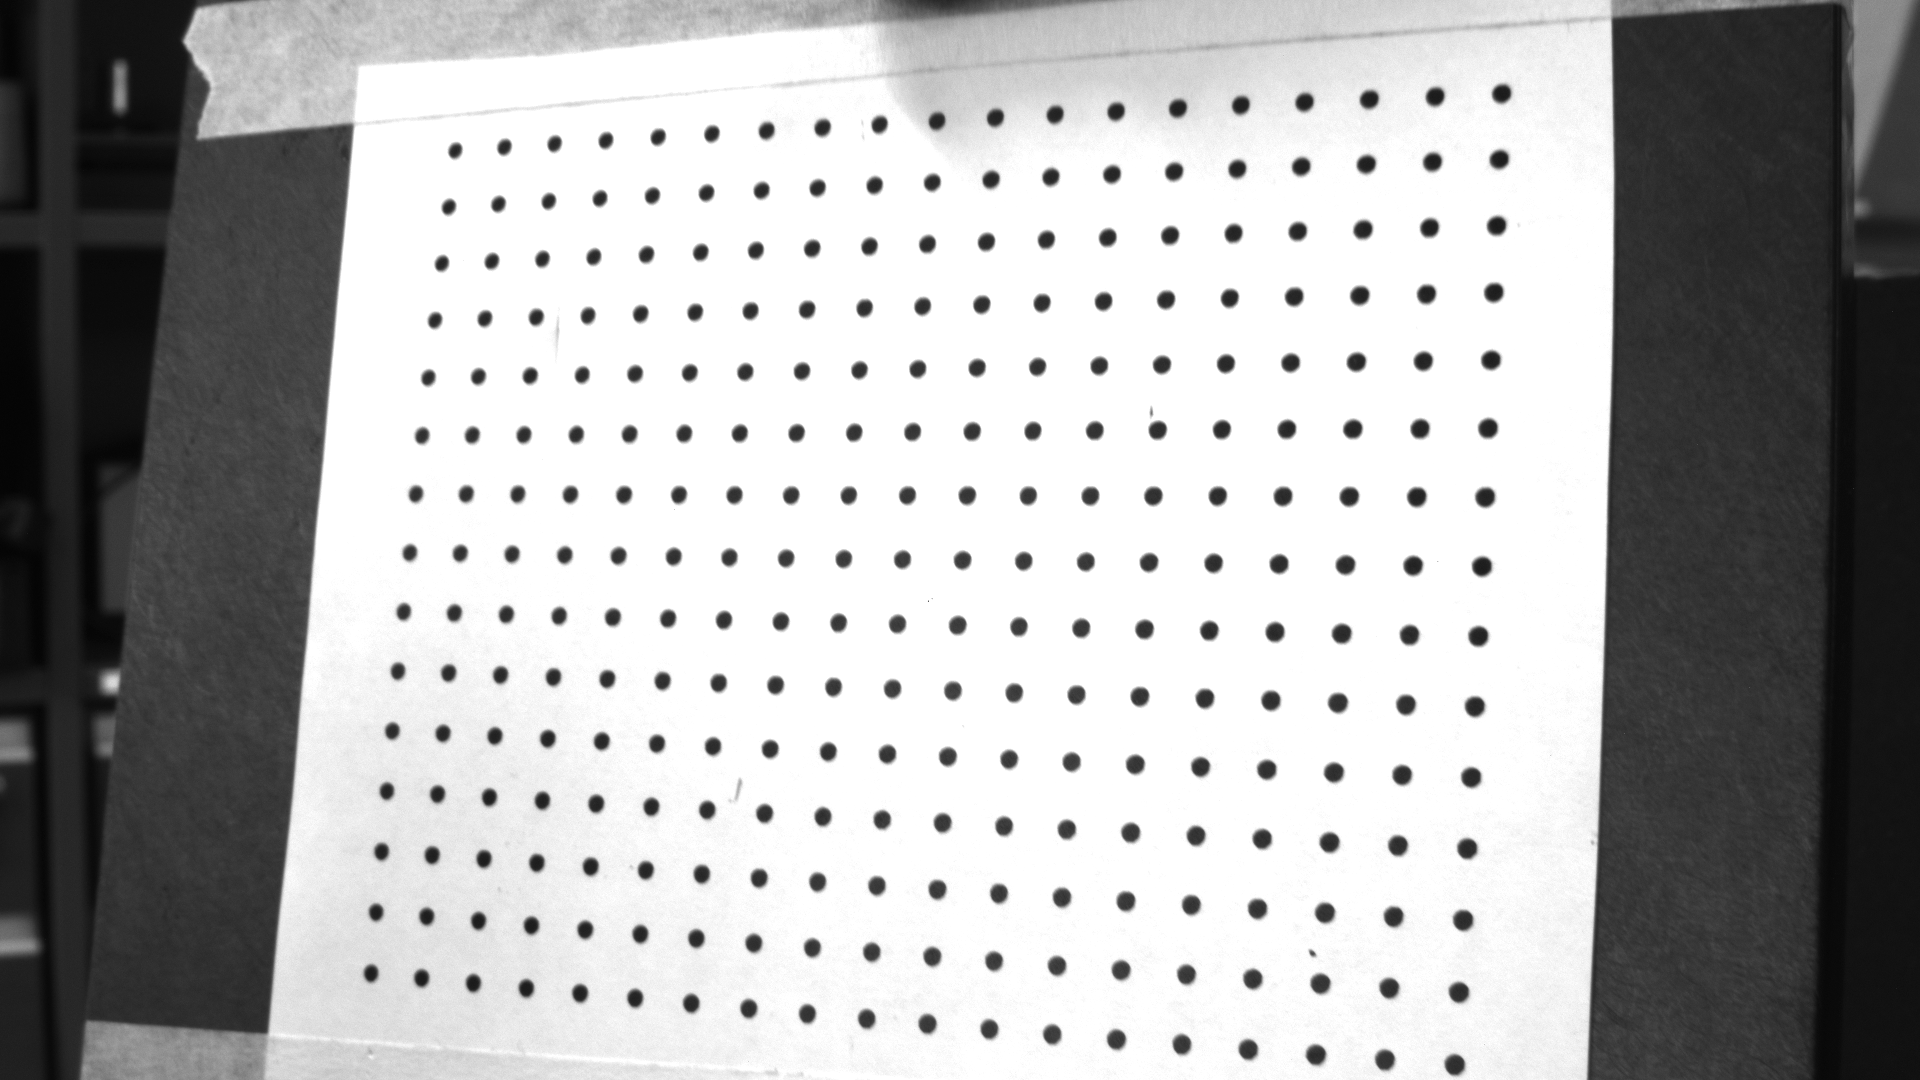
\includegraphics[width=0.49\linewidth]{scans/calibration_camera/GE1910/20141105154814726}
        }
       \subfloat{
            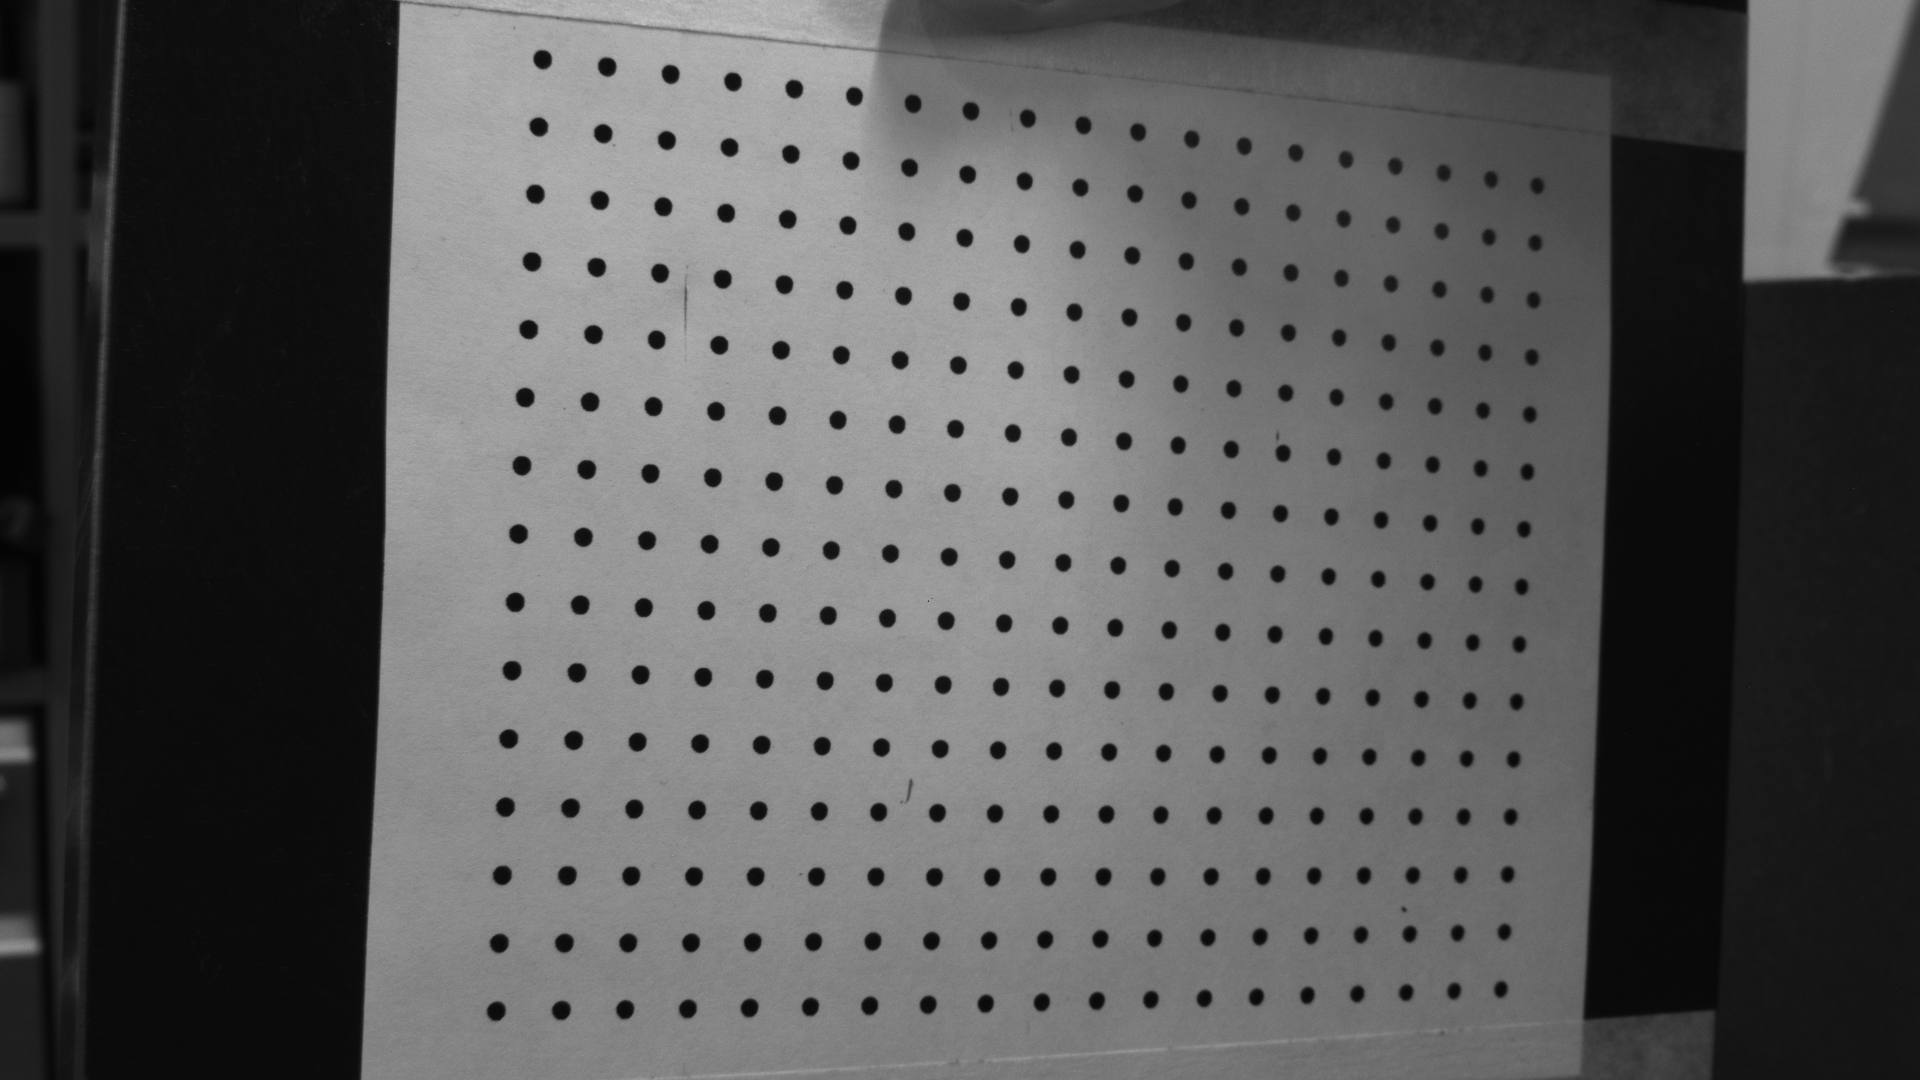
\includegraphics[width=0.49\linewidth]{scans/calibration_camera/GE1910/20141105154934766}
        }
       \\
        \subfloat{
            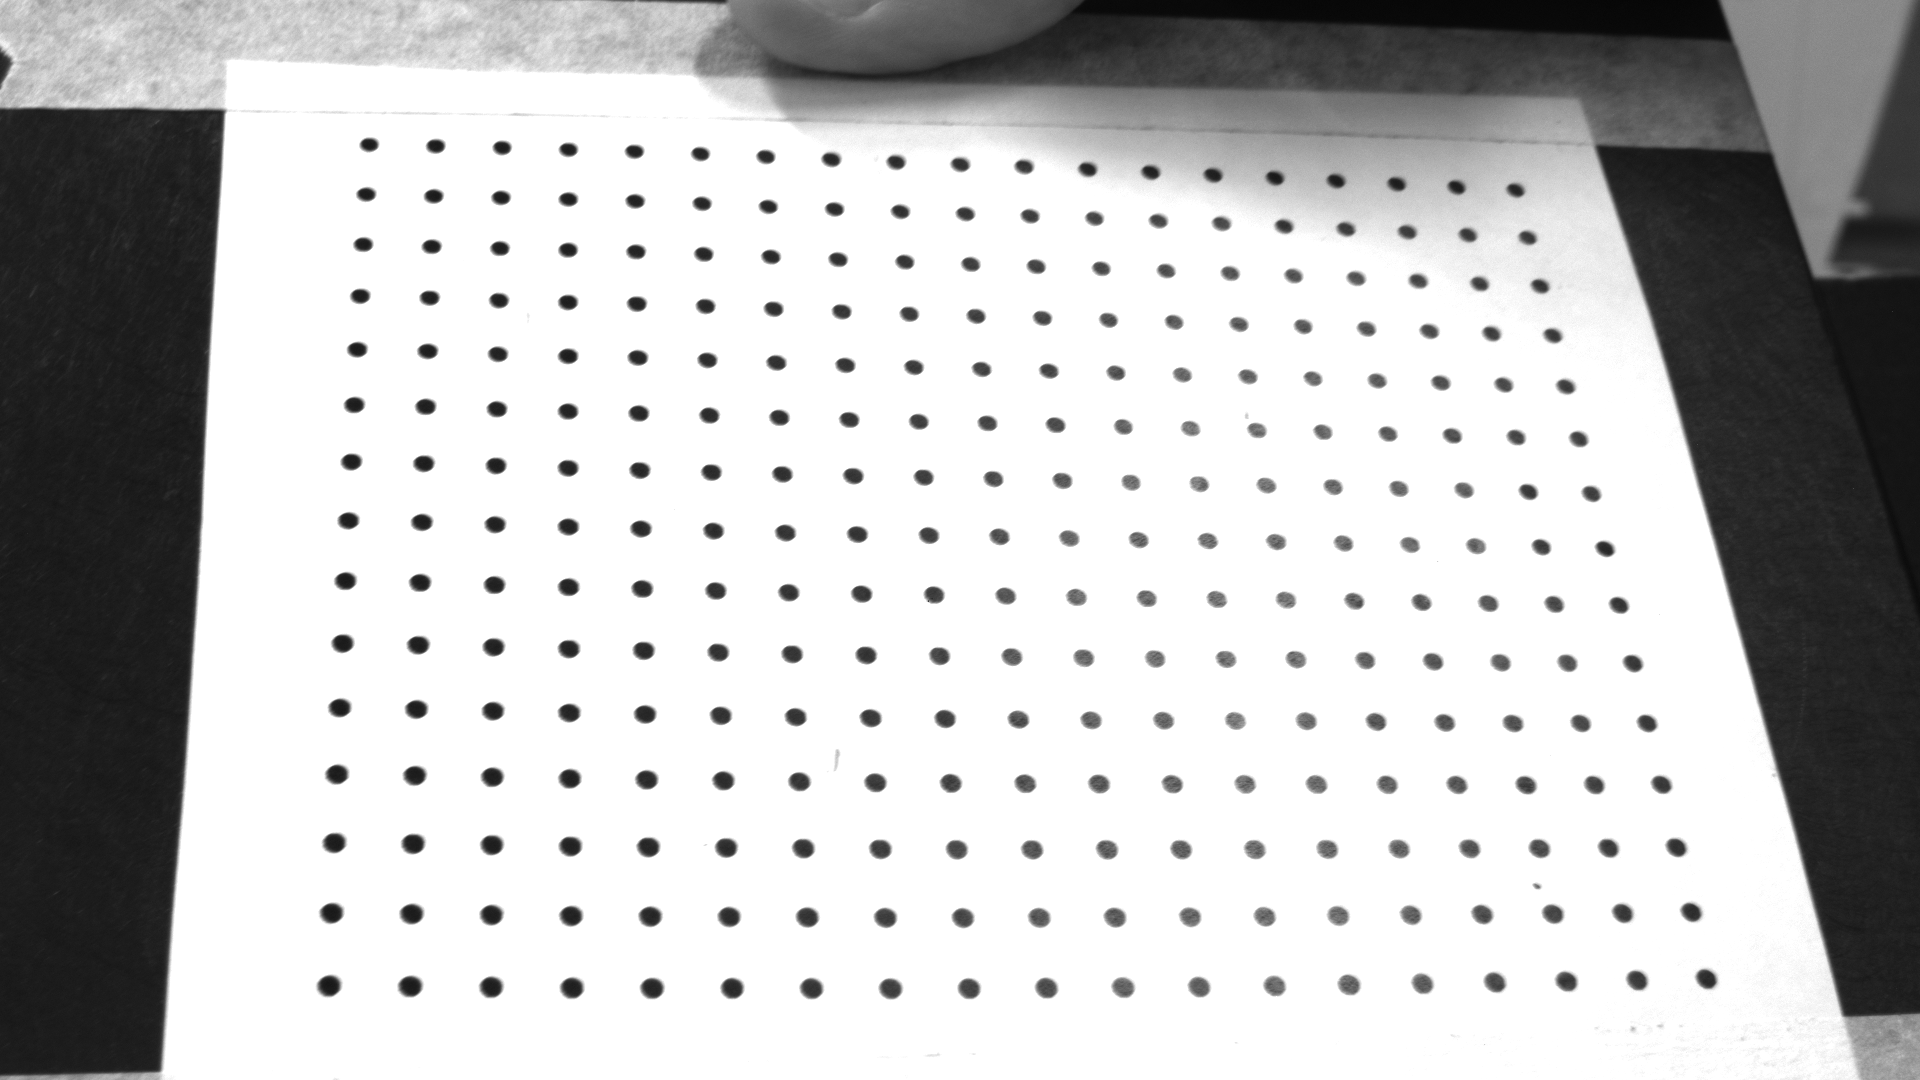
\includegraphics[width=0.49\linewidth]{scans/calibration_camera/GE1910/20141105154944097}
        }
       \subfloat{
            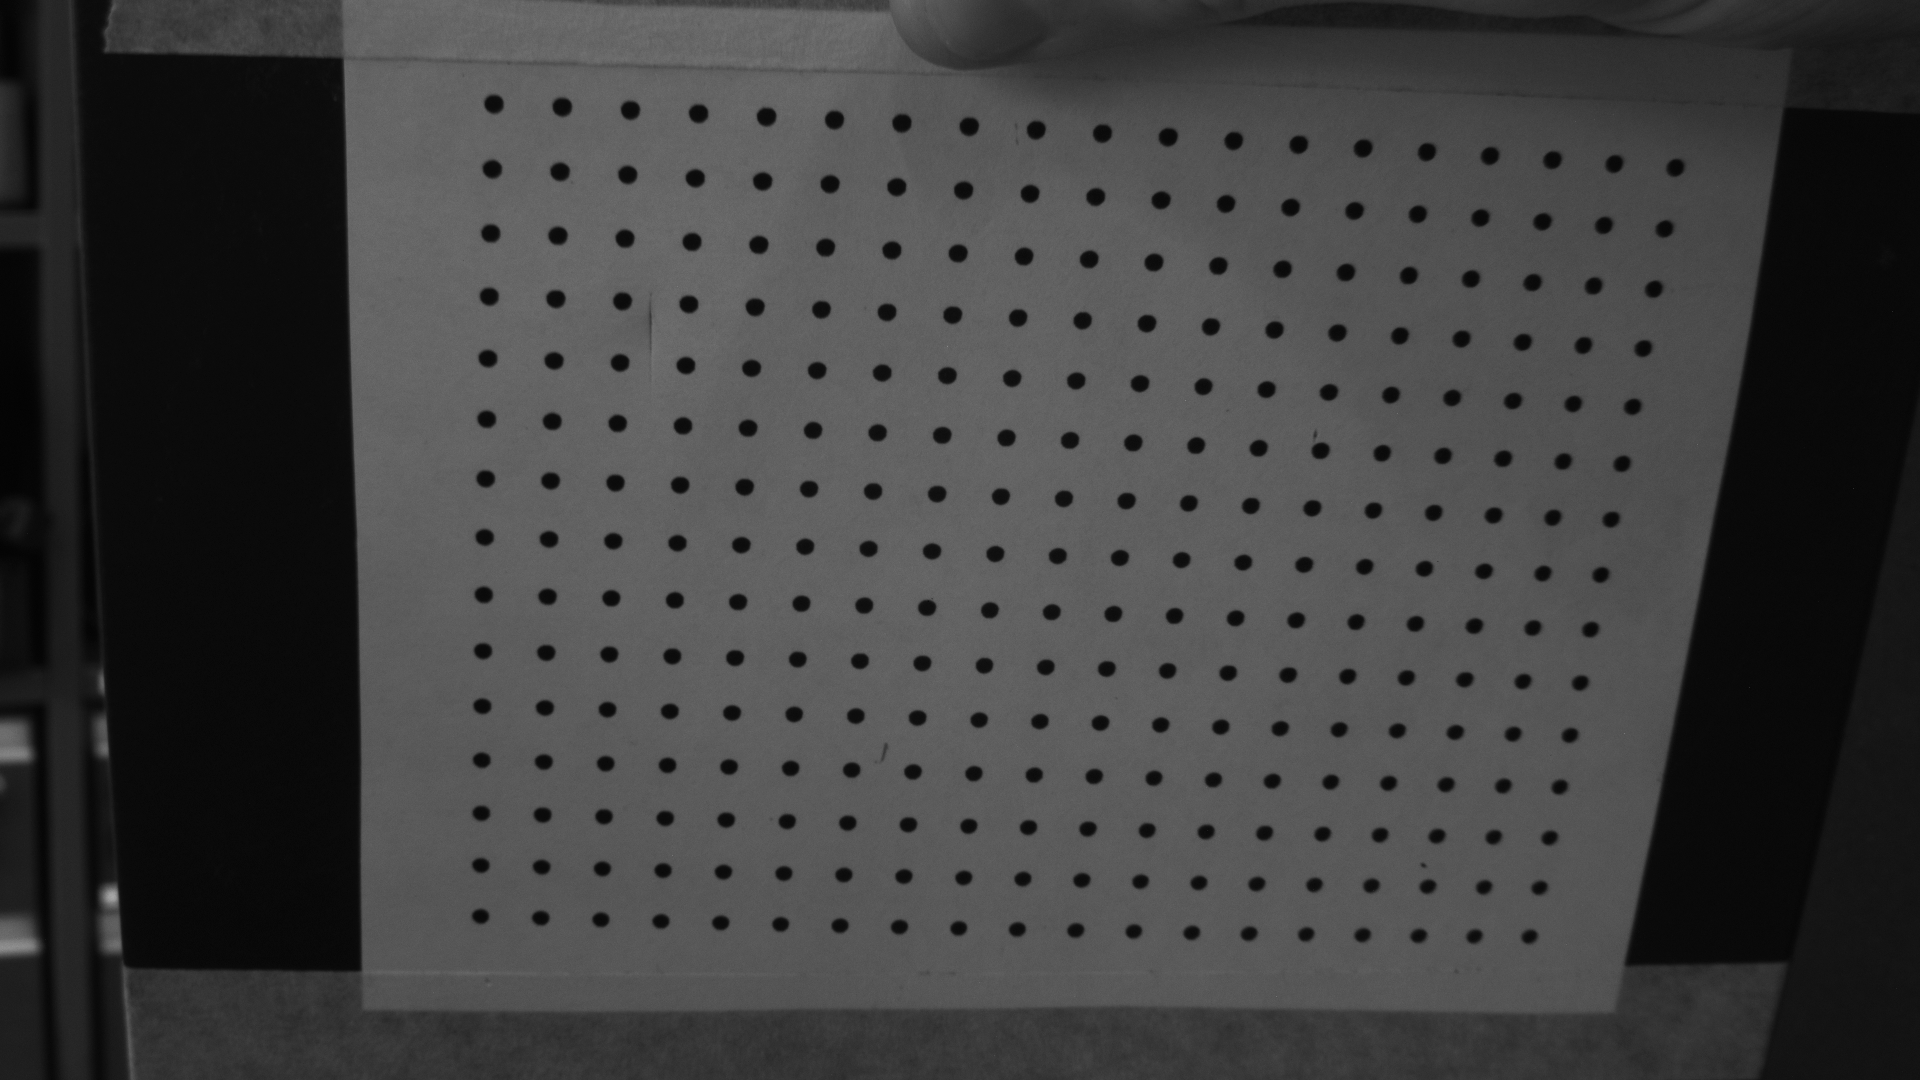
\includegraphics[width=0.49\linewidth]{scans/calibration_camera/GE1910/20141105154954098}
        }
        \\
        \subfloat{
            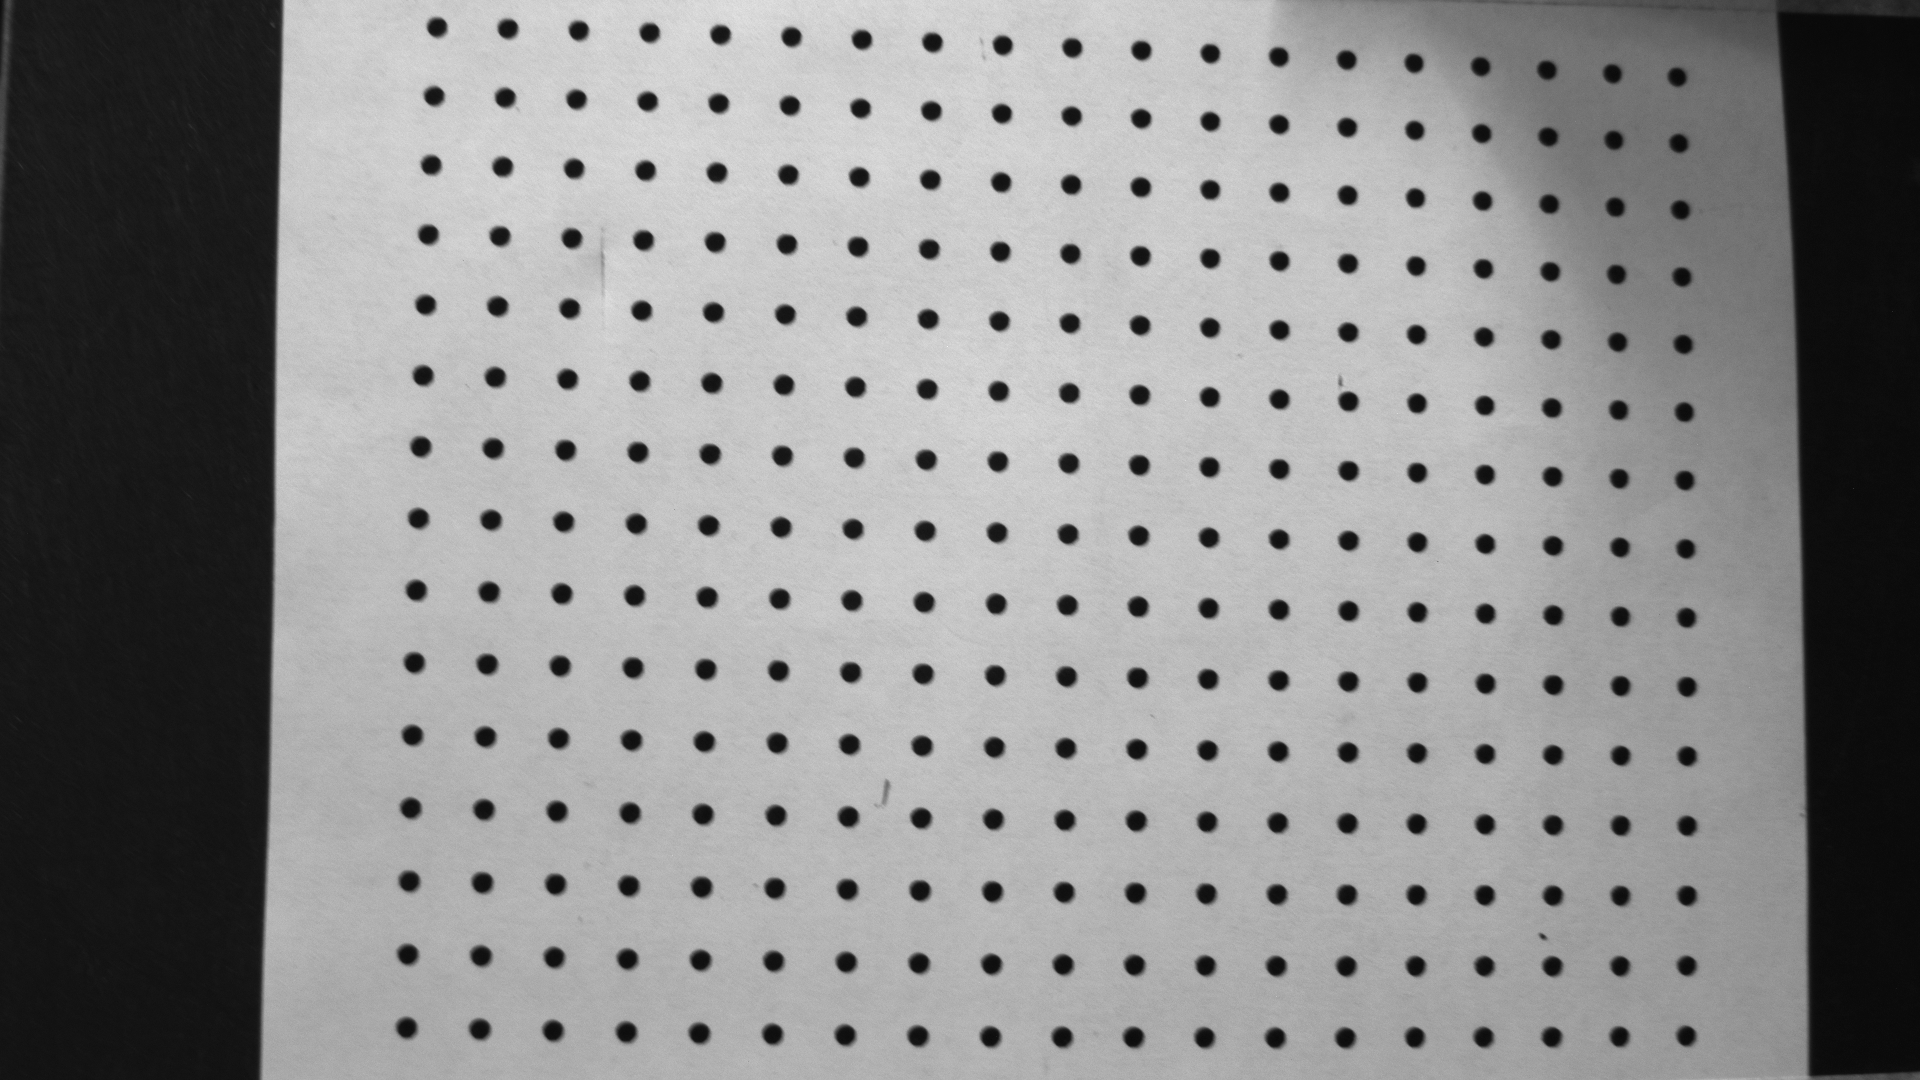
\includegraphics[width=0.49\linewidth]{scans/calibration_camera/GE1910/20141105154745404}
        }
        \caption{Imagenes de calibración para la cámara izquierda}
        \label{fig:calibrationImagesGE1910}
\end{figure}

\begin{figure}[!bth]
    \myfloatalign
        \subfloat{
            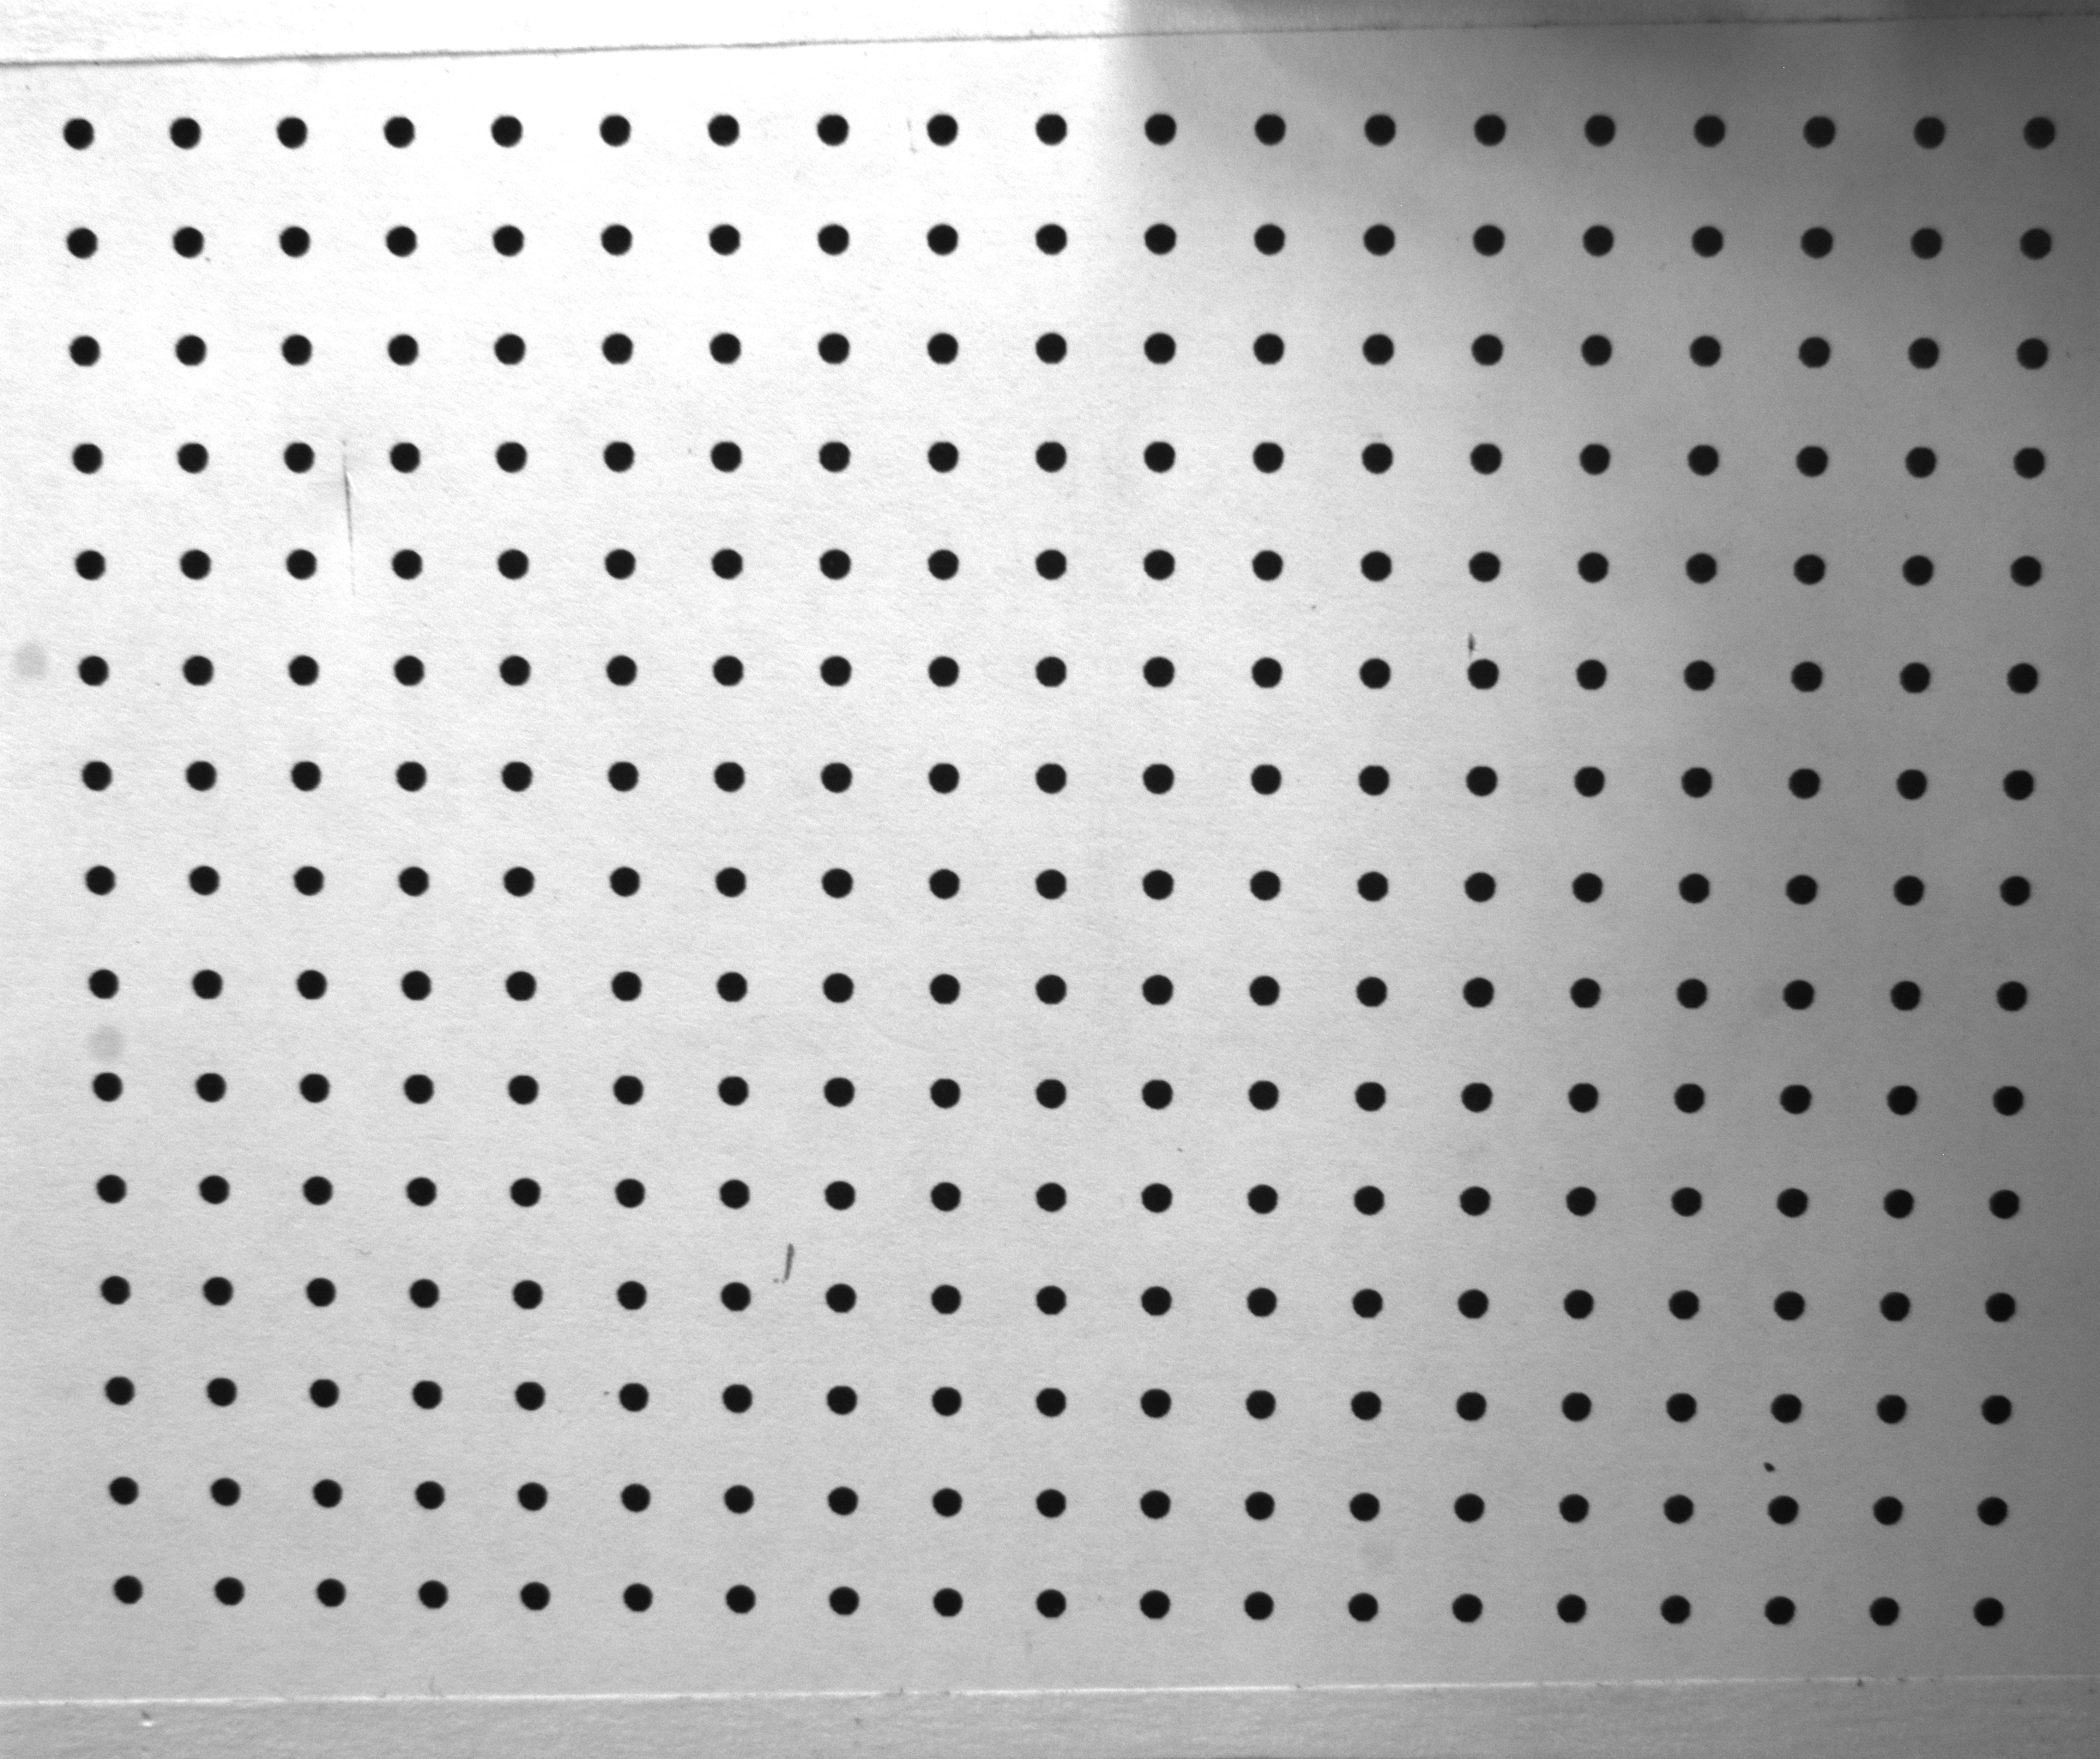
\includegraphics[width=0.49\linewidth]{scans/calibration_camera/GC2450M/20141105155838231}
        }
       \subfloat{
            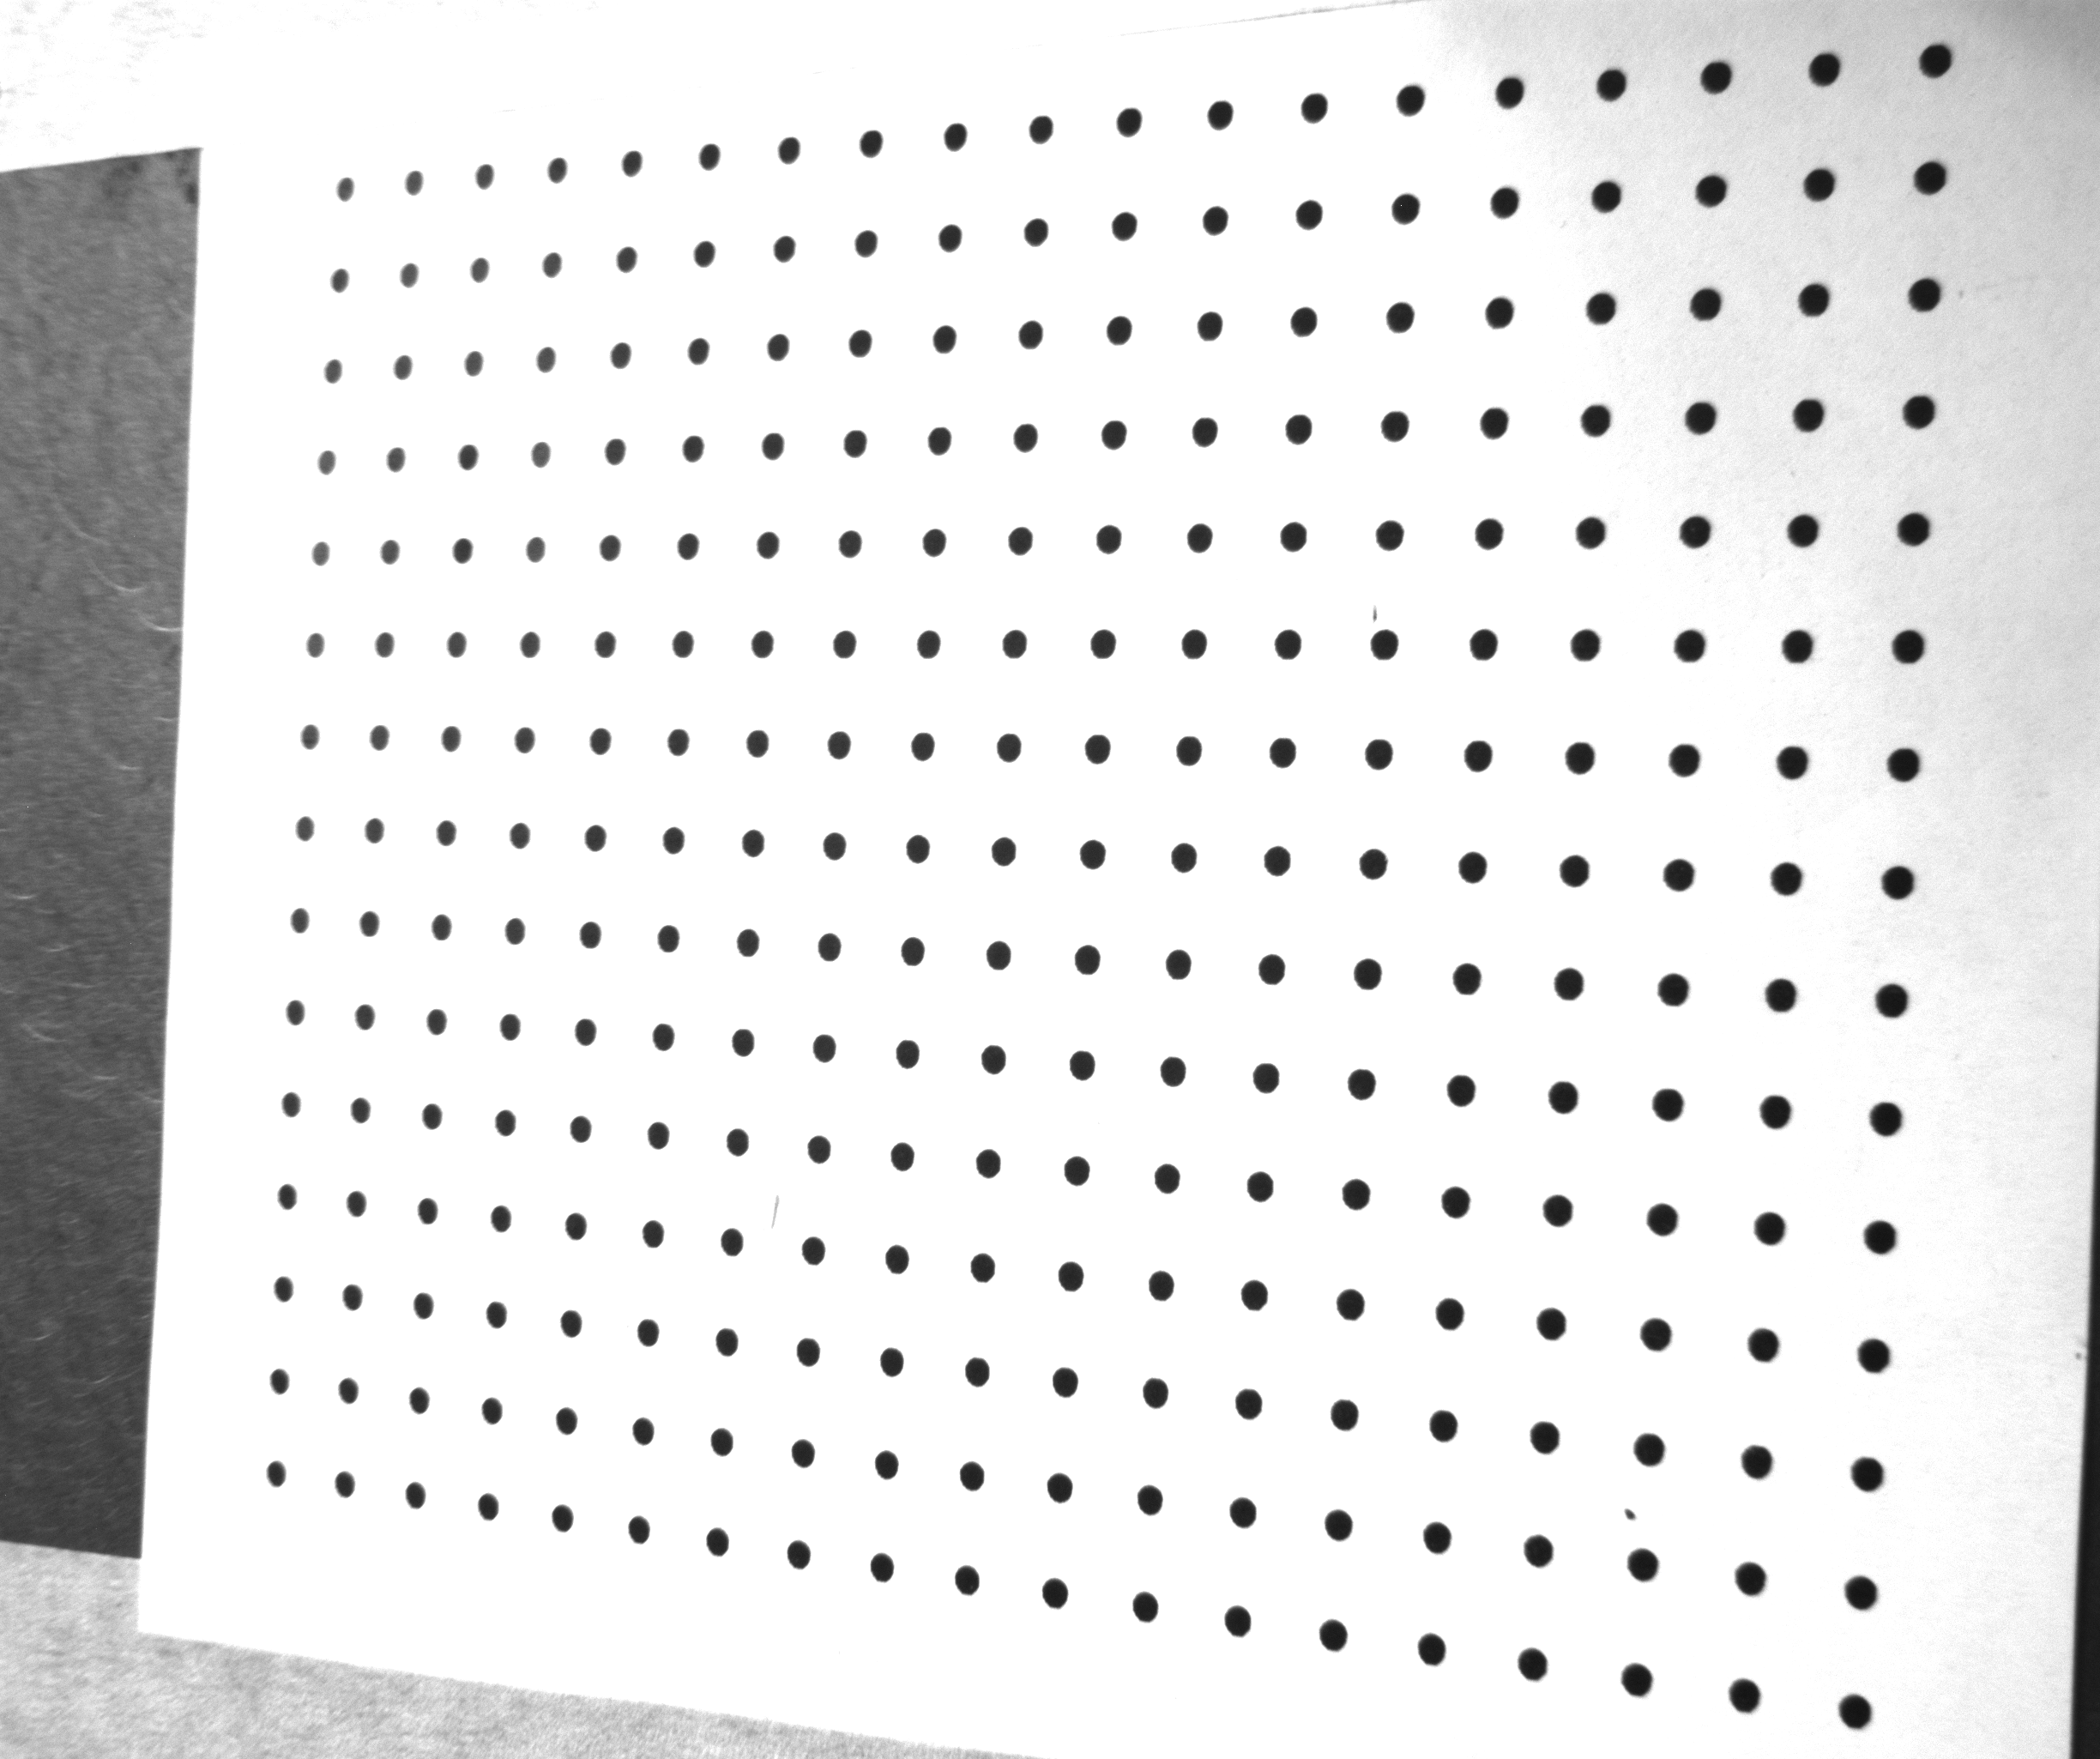
\includegraphics[width=0.49\linewidth]{scans/calibration_camera/GC2450M/20141105155855073}
        }
       \\
        \subfloat{
            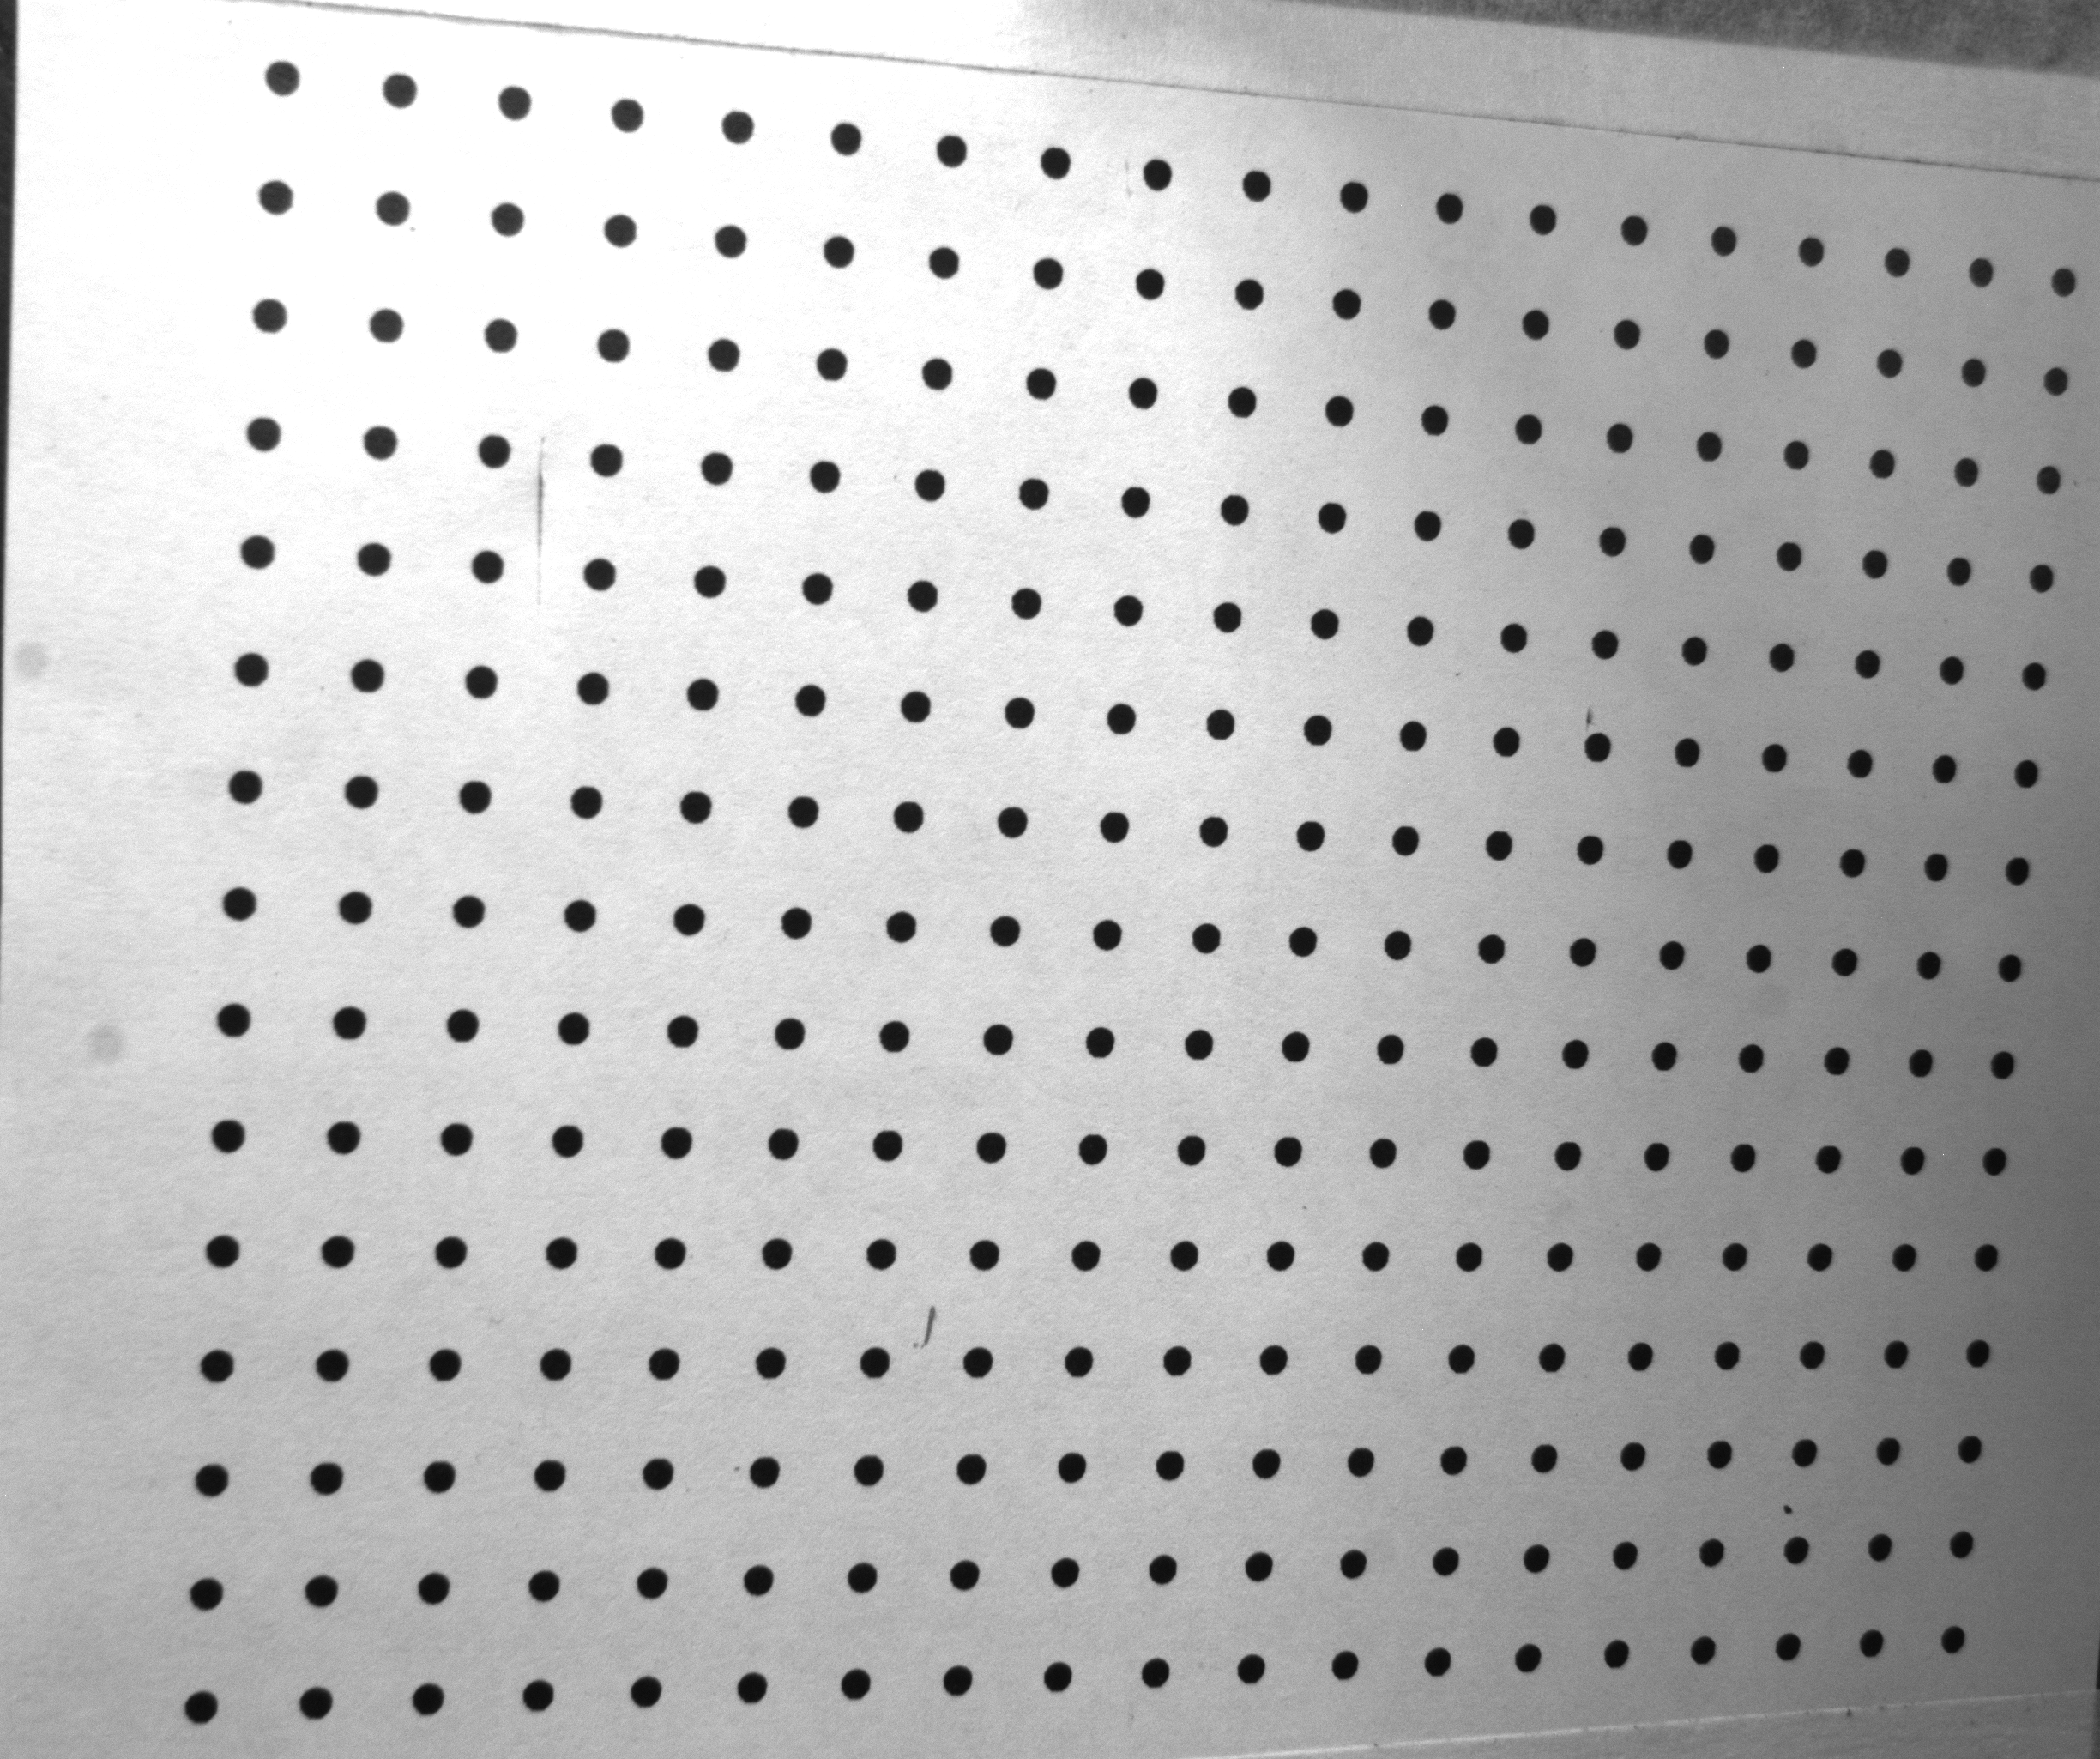
\includegraphics[width=0.49\linewidth]{scans/calibration_camera/GC2450M/20141105155916202}
        }
       \subfloat{
            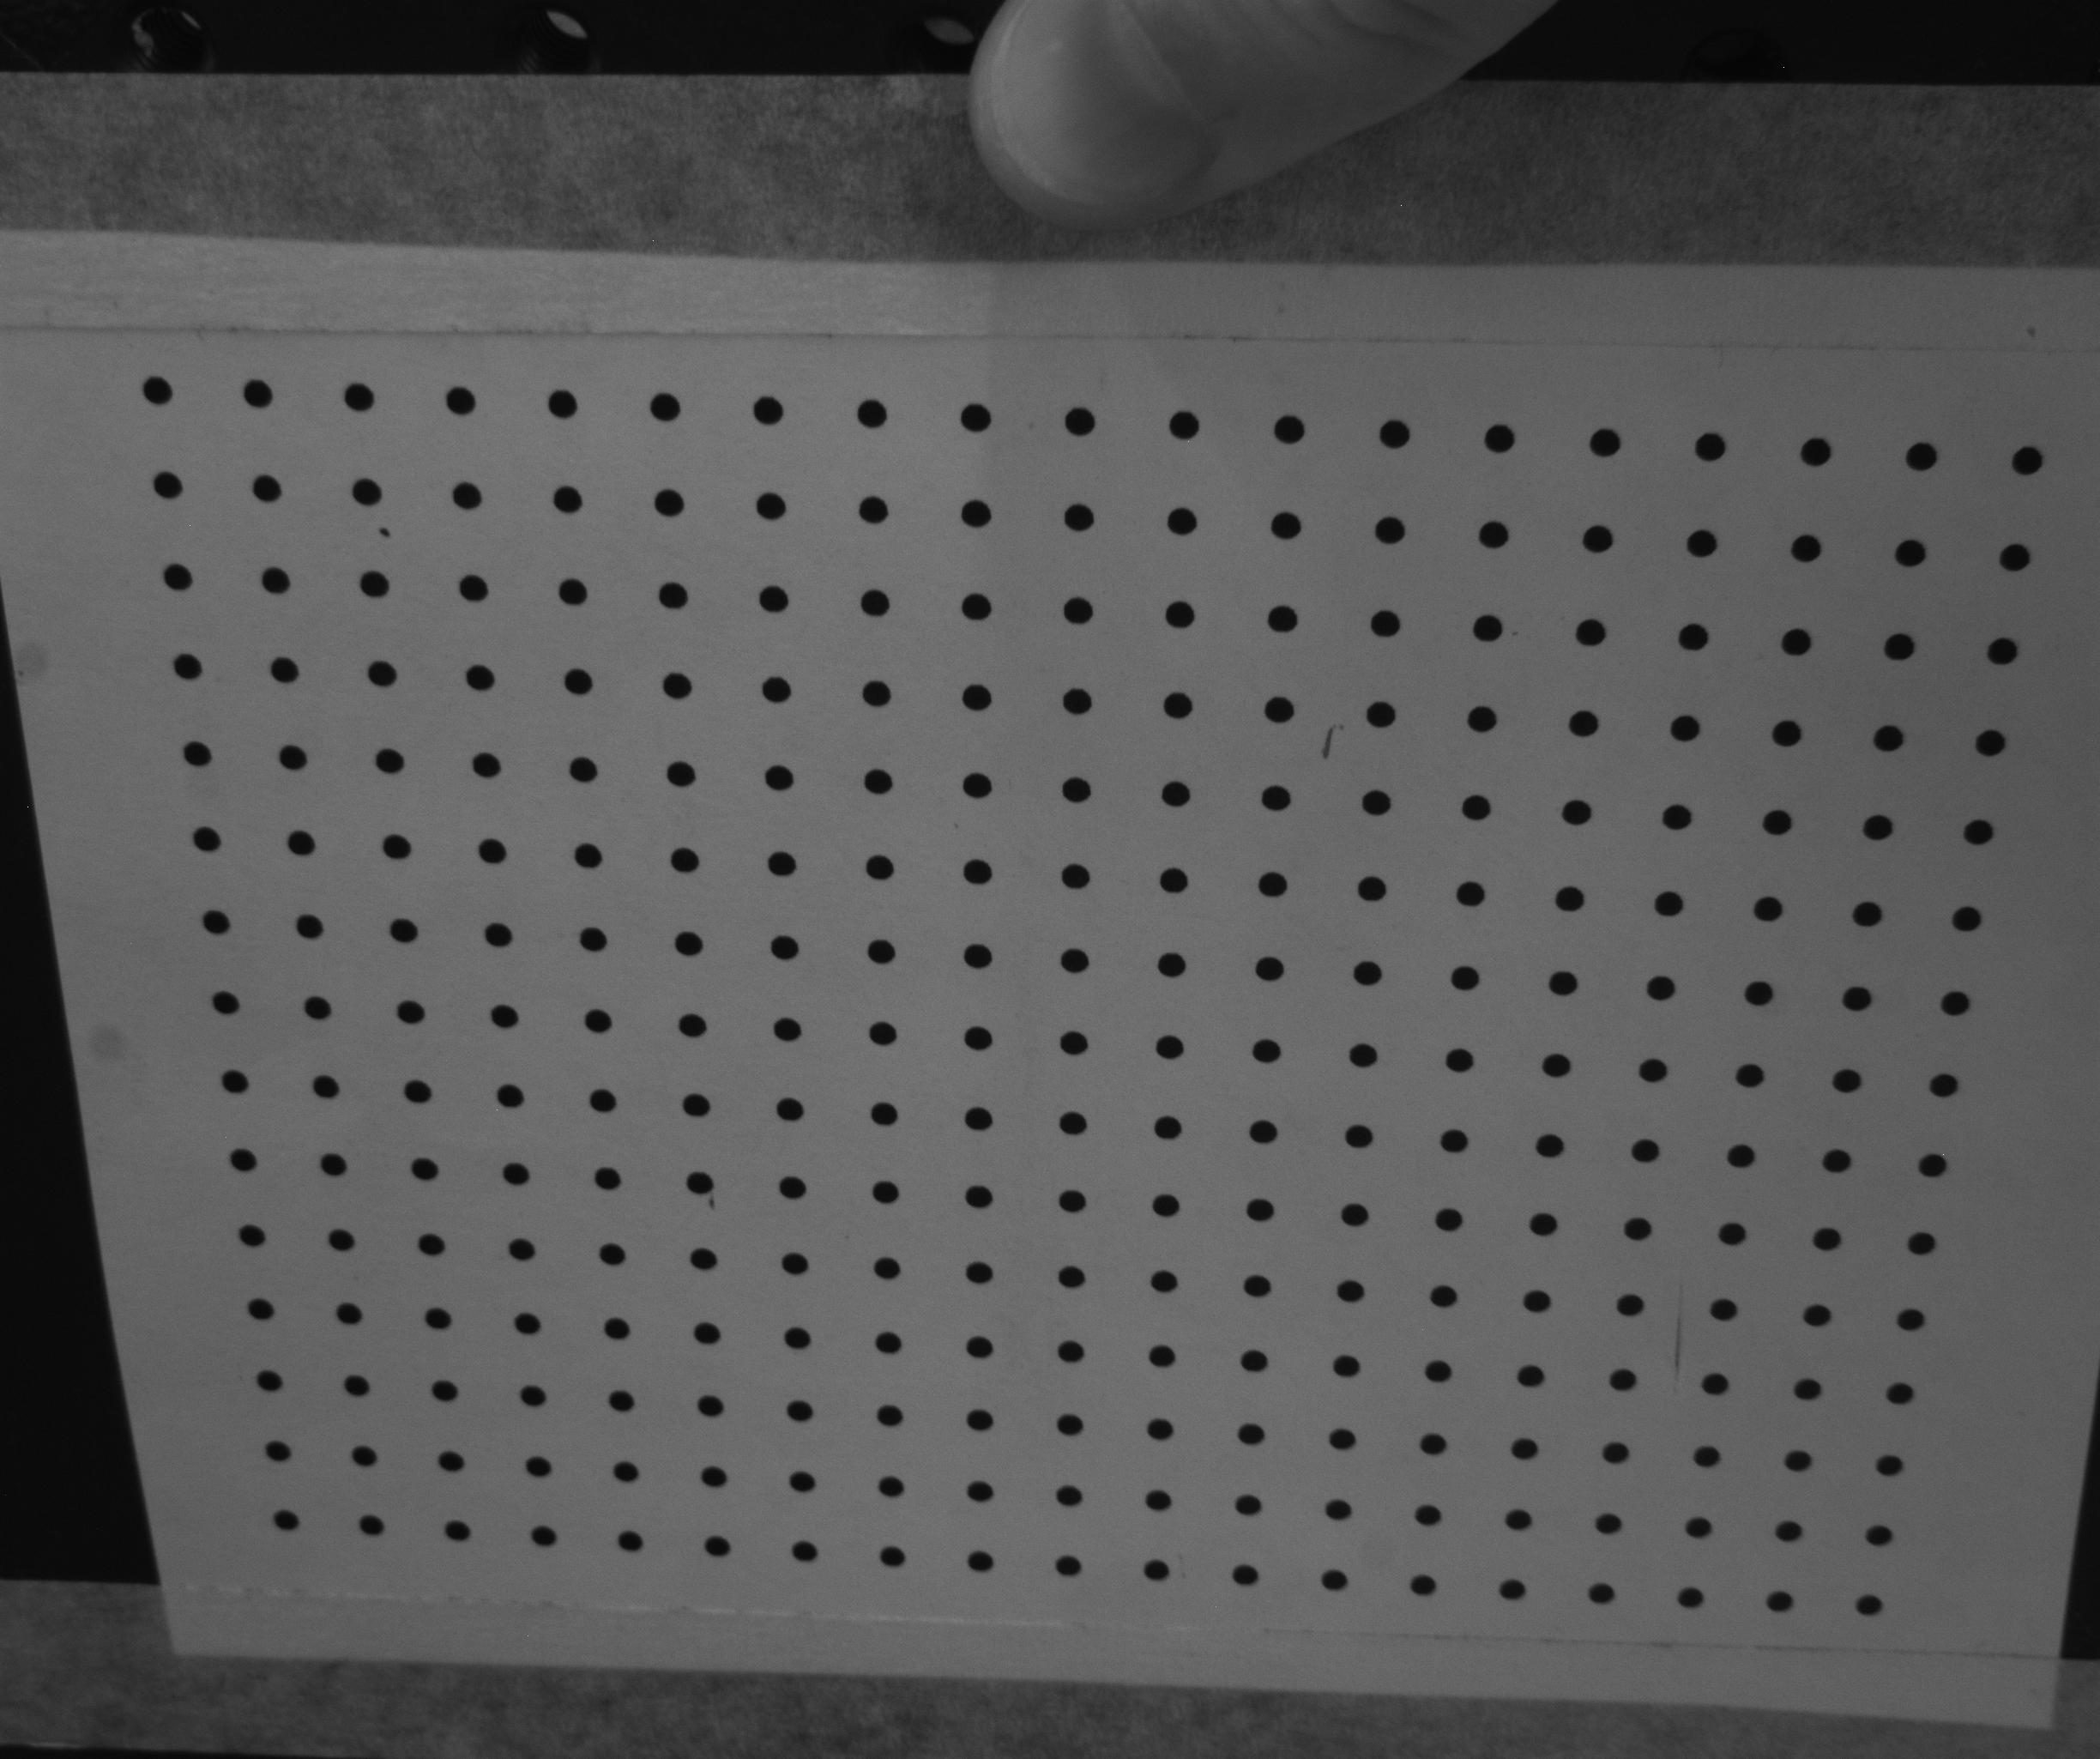
\includegraphics[width=0.49\linewidth]{scans/calibration_camera/GC2450M/20141105160229979}
        }
        \caption{Imagenes de calibración para la cámara derecha}
        \label{fig:calibrationImagesGC2450M}
\end{figure}

Para la obtención de la relación entre una cámara y la otra se deben obtener imágenes simultaneas desde cada cámara, en cada una de las cuales se debe observar el patrón de calibración. En este caso el patrón de calibración es similar pero de un menor tamaño, con una grilla de círculos de 15x11, para facilitar la vista simultánea desde ambas cámaras en diversas ubicaciones. Las imágenes utilizadas se pueden observar en la \autoref{fig:stereoCalibrationImages2}.
%las figuras  \ref{fig:stereoCalibrationImages1} y \ref{fig:stereoCalibrationImages2}.

\begin{figure}[!bth]
    \myfloatalign
        \subfloat{
            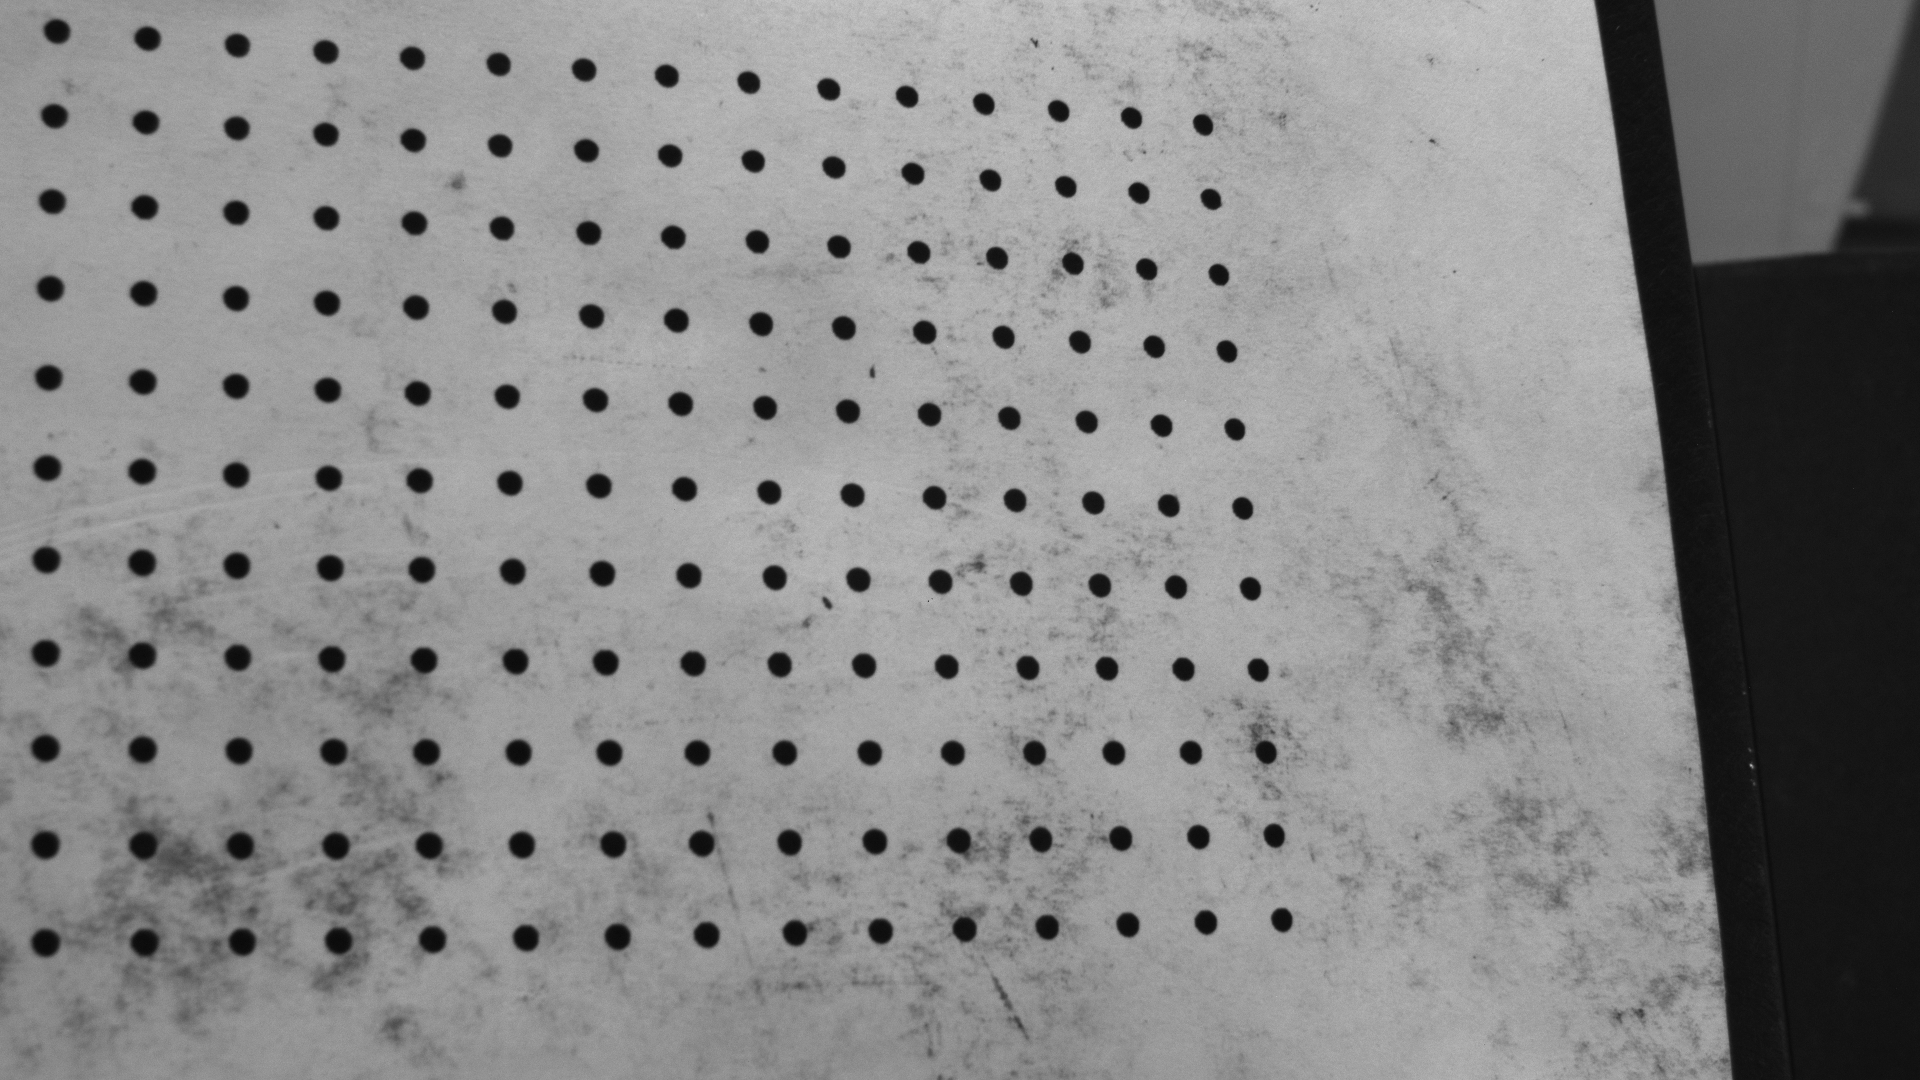
\includegraphics[width=0.52\linewidth]{scans/calibration_stereo/GE1910/20141105161703}
        }
       \subfloat{
            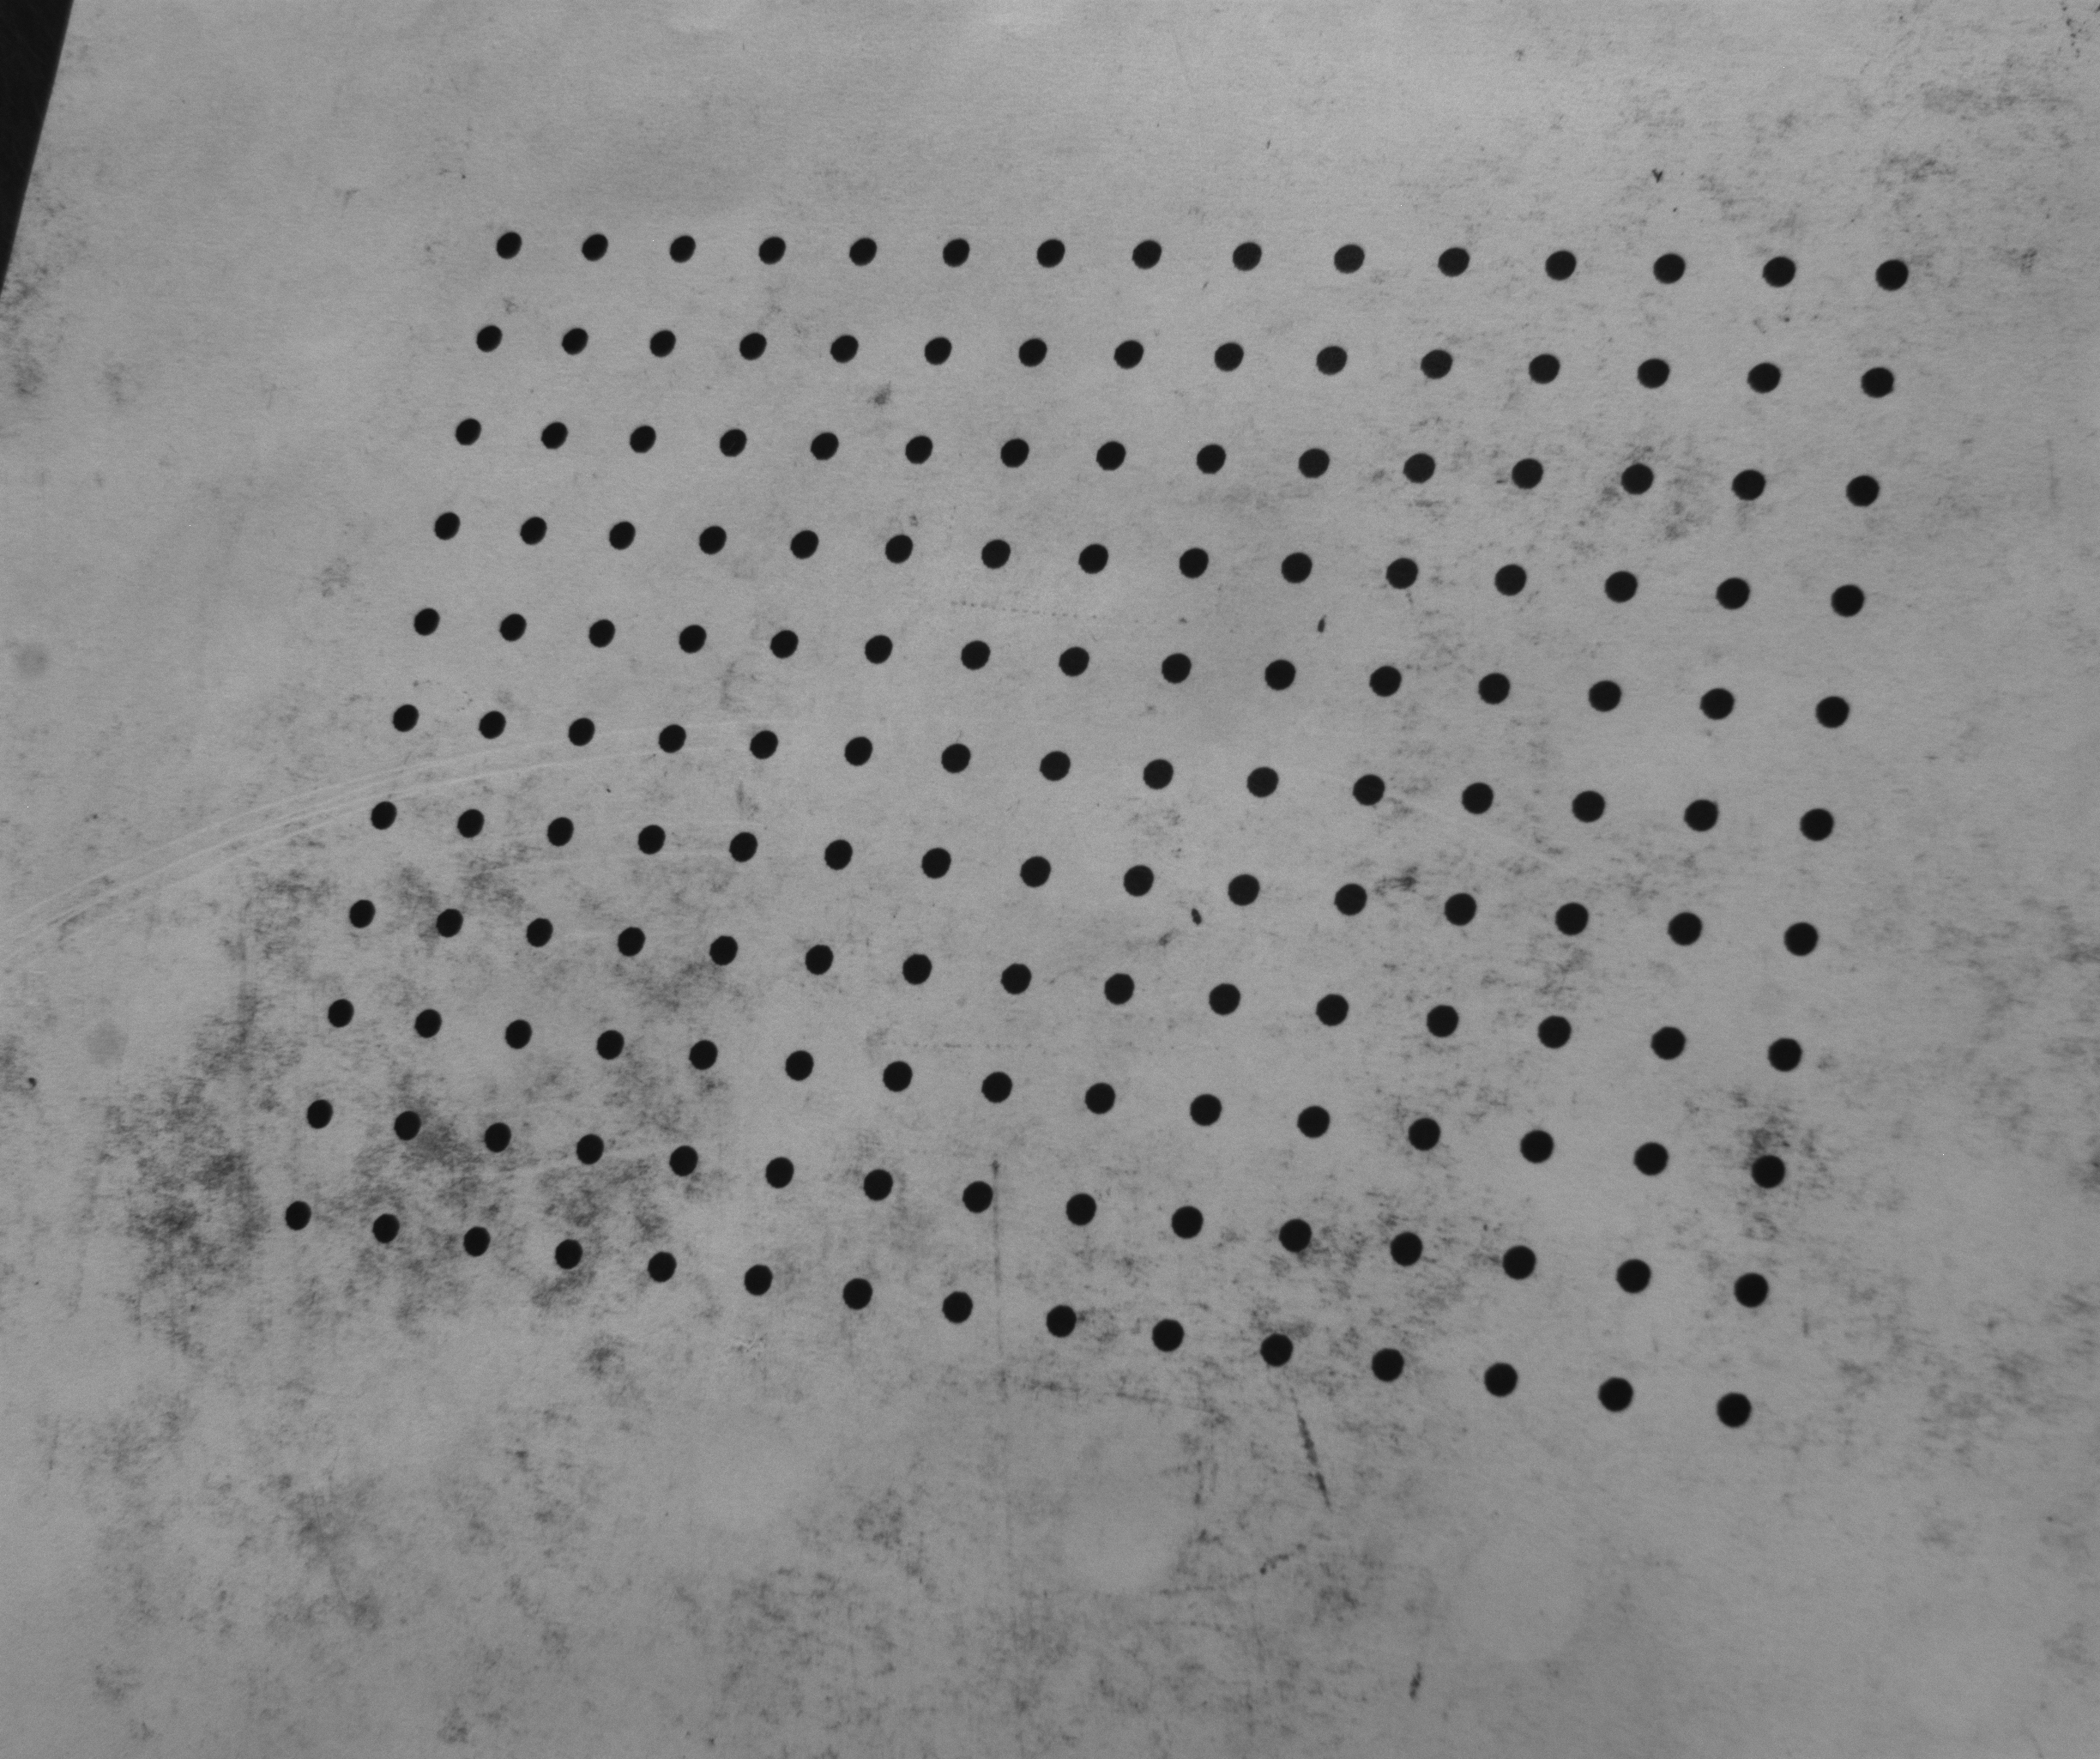
\includegraphics[width=0.35\linewidth]{scans/calibration_stereo/GC2450M/20141105161703}
        }
       \\
        \subfloat{
            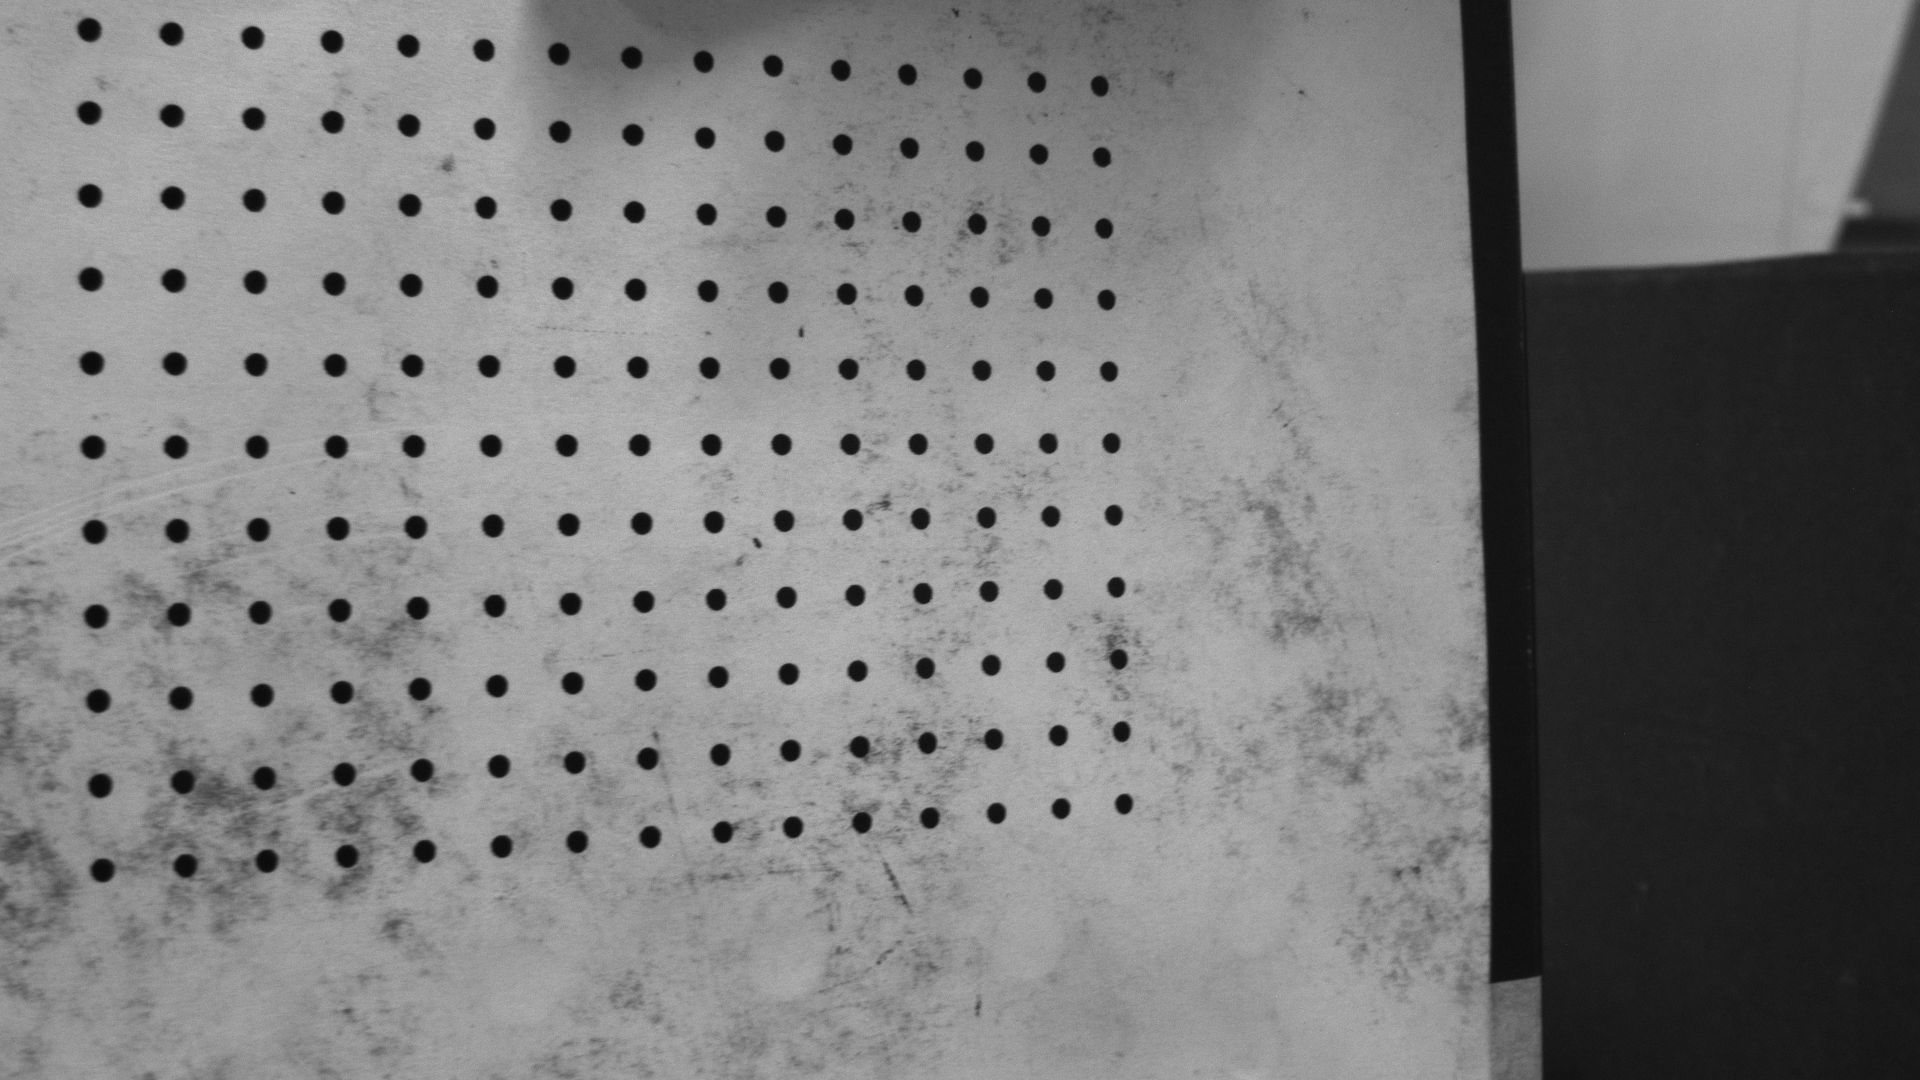
\includegraphics[width=0.52\linewidth]{scans/calibration_stereo/GE1910/20141105161923}
        }
       \subfloat{
            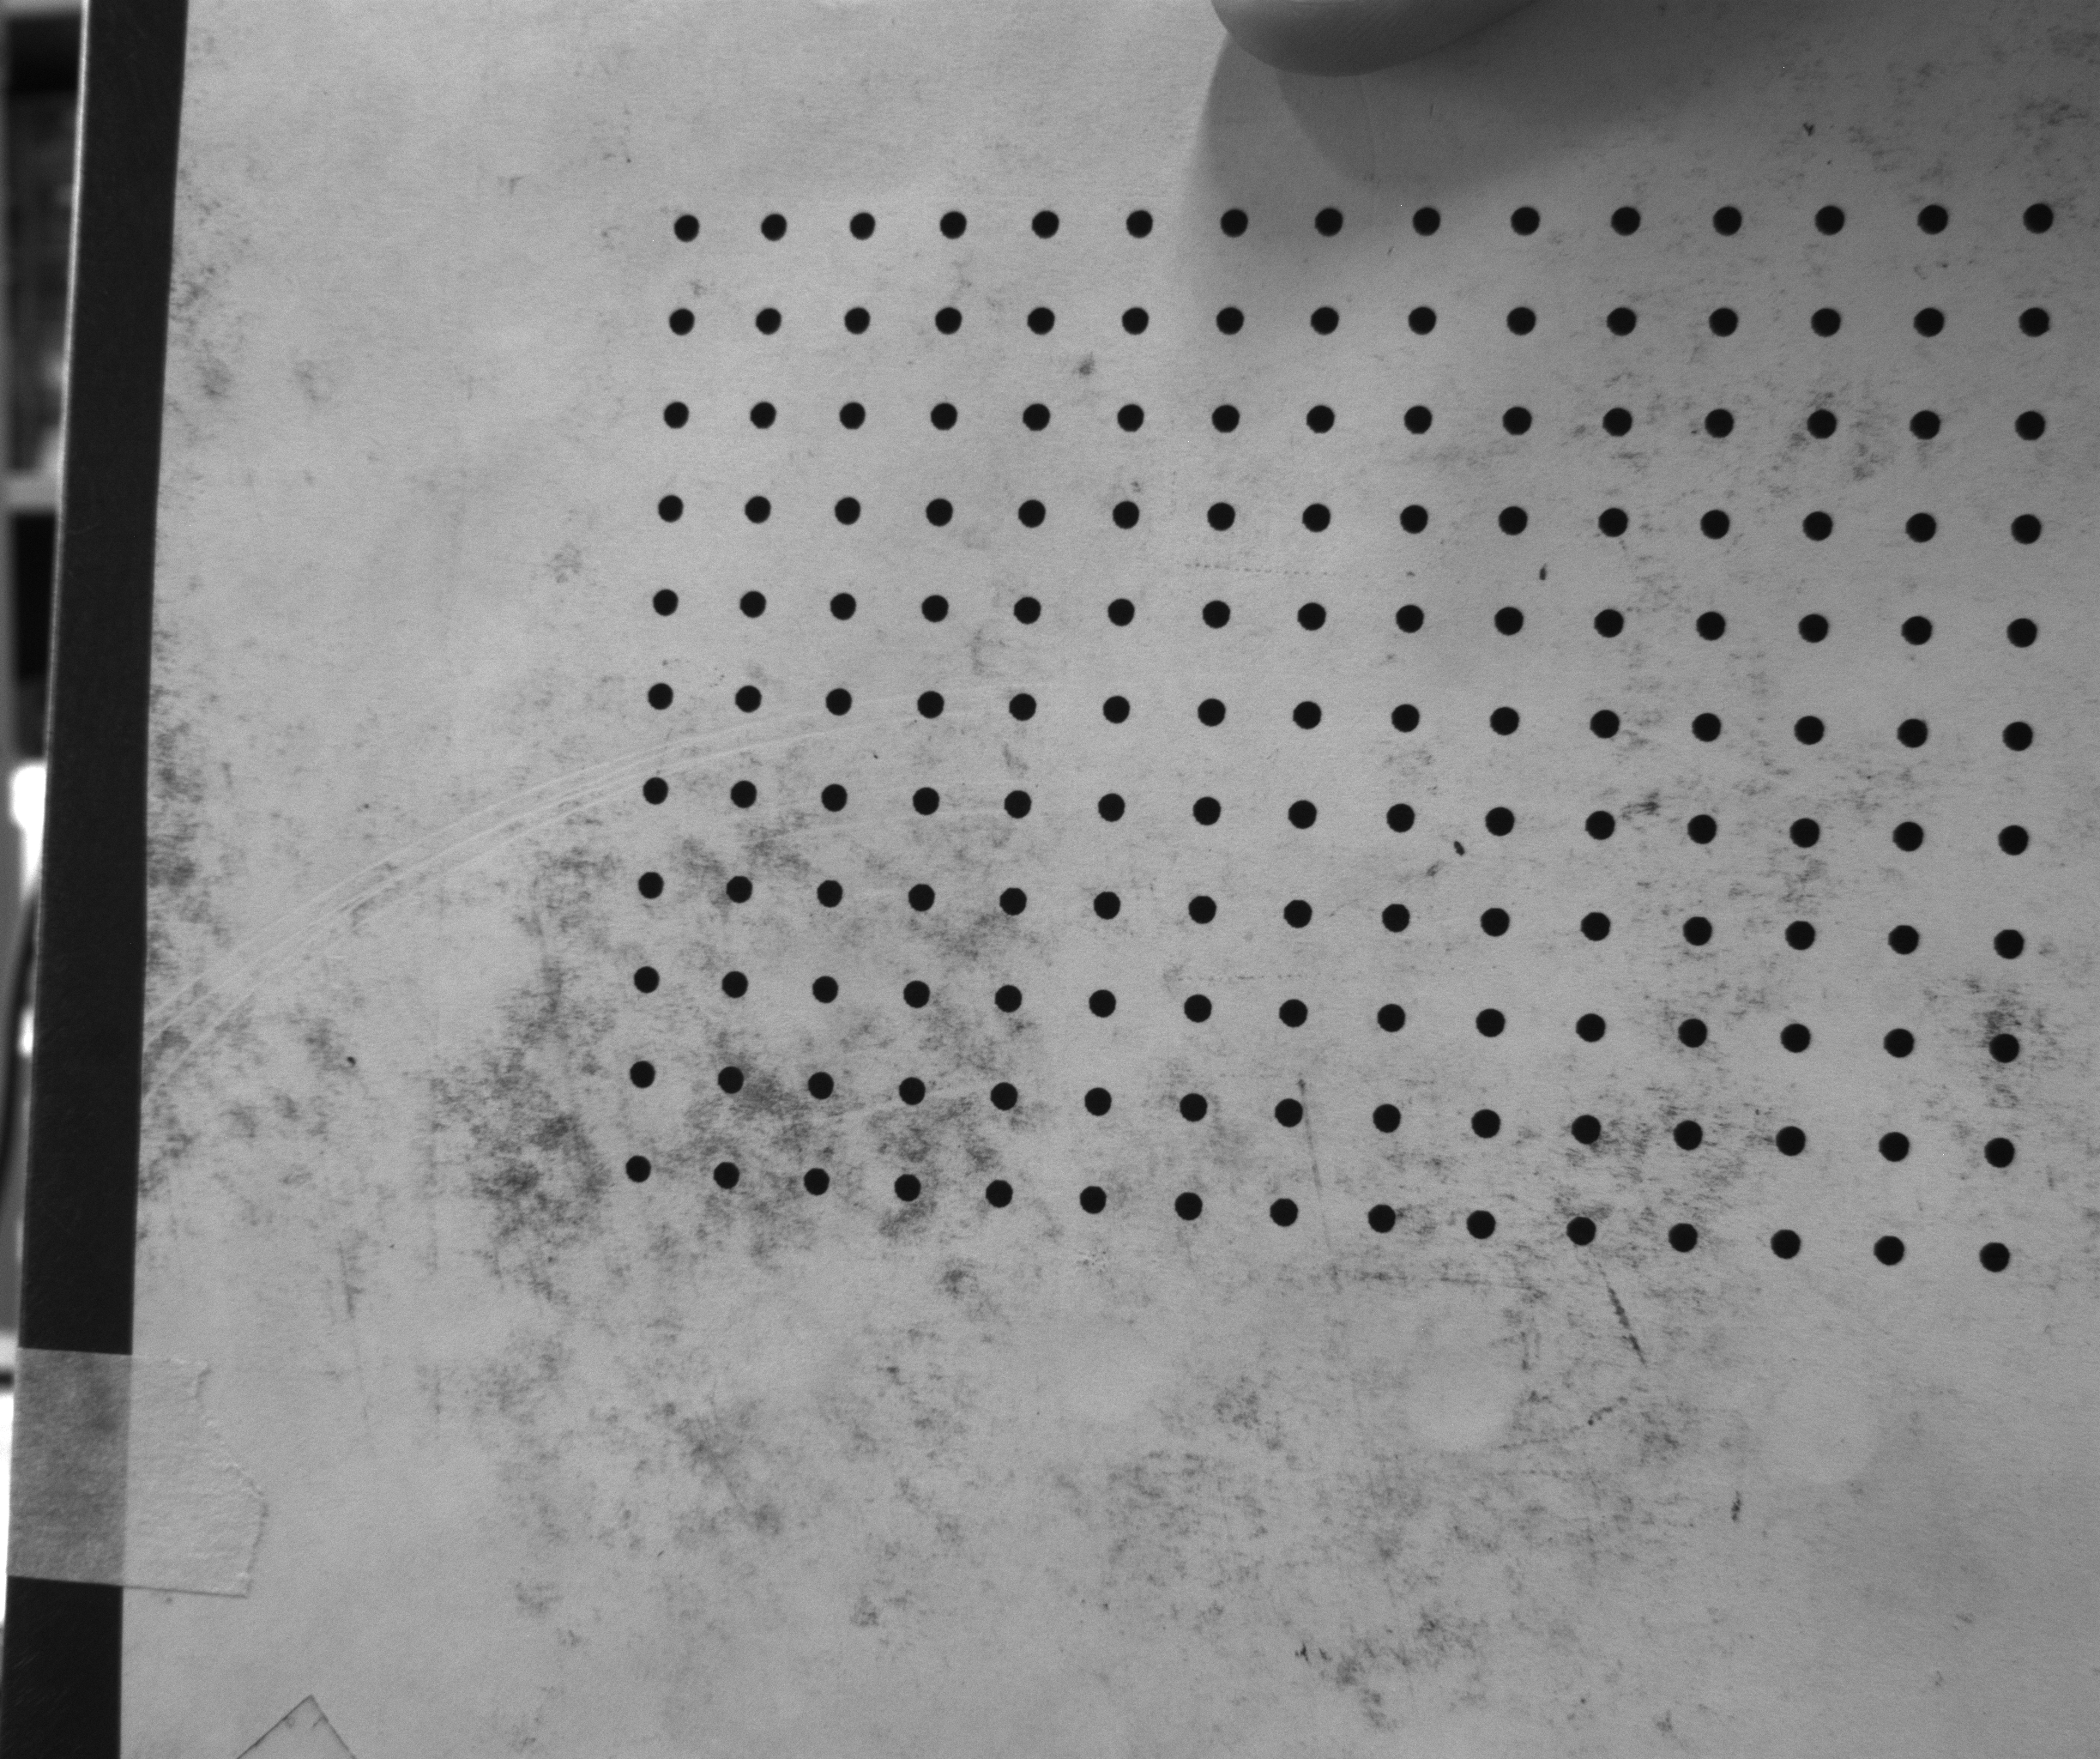
\includegraphics[width=0.35\linewidth]{scans/calibration_stereo/GC2450M/20141105161923}
        }
       \\
        \subfloat{
            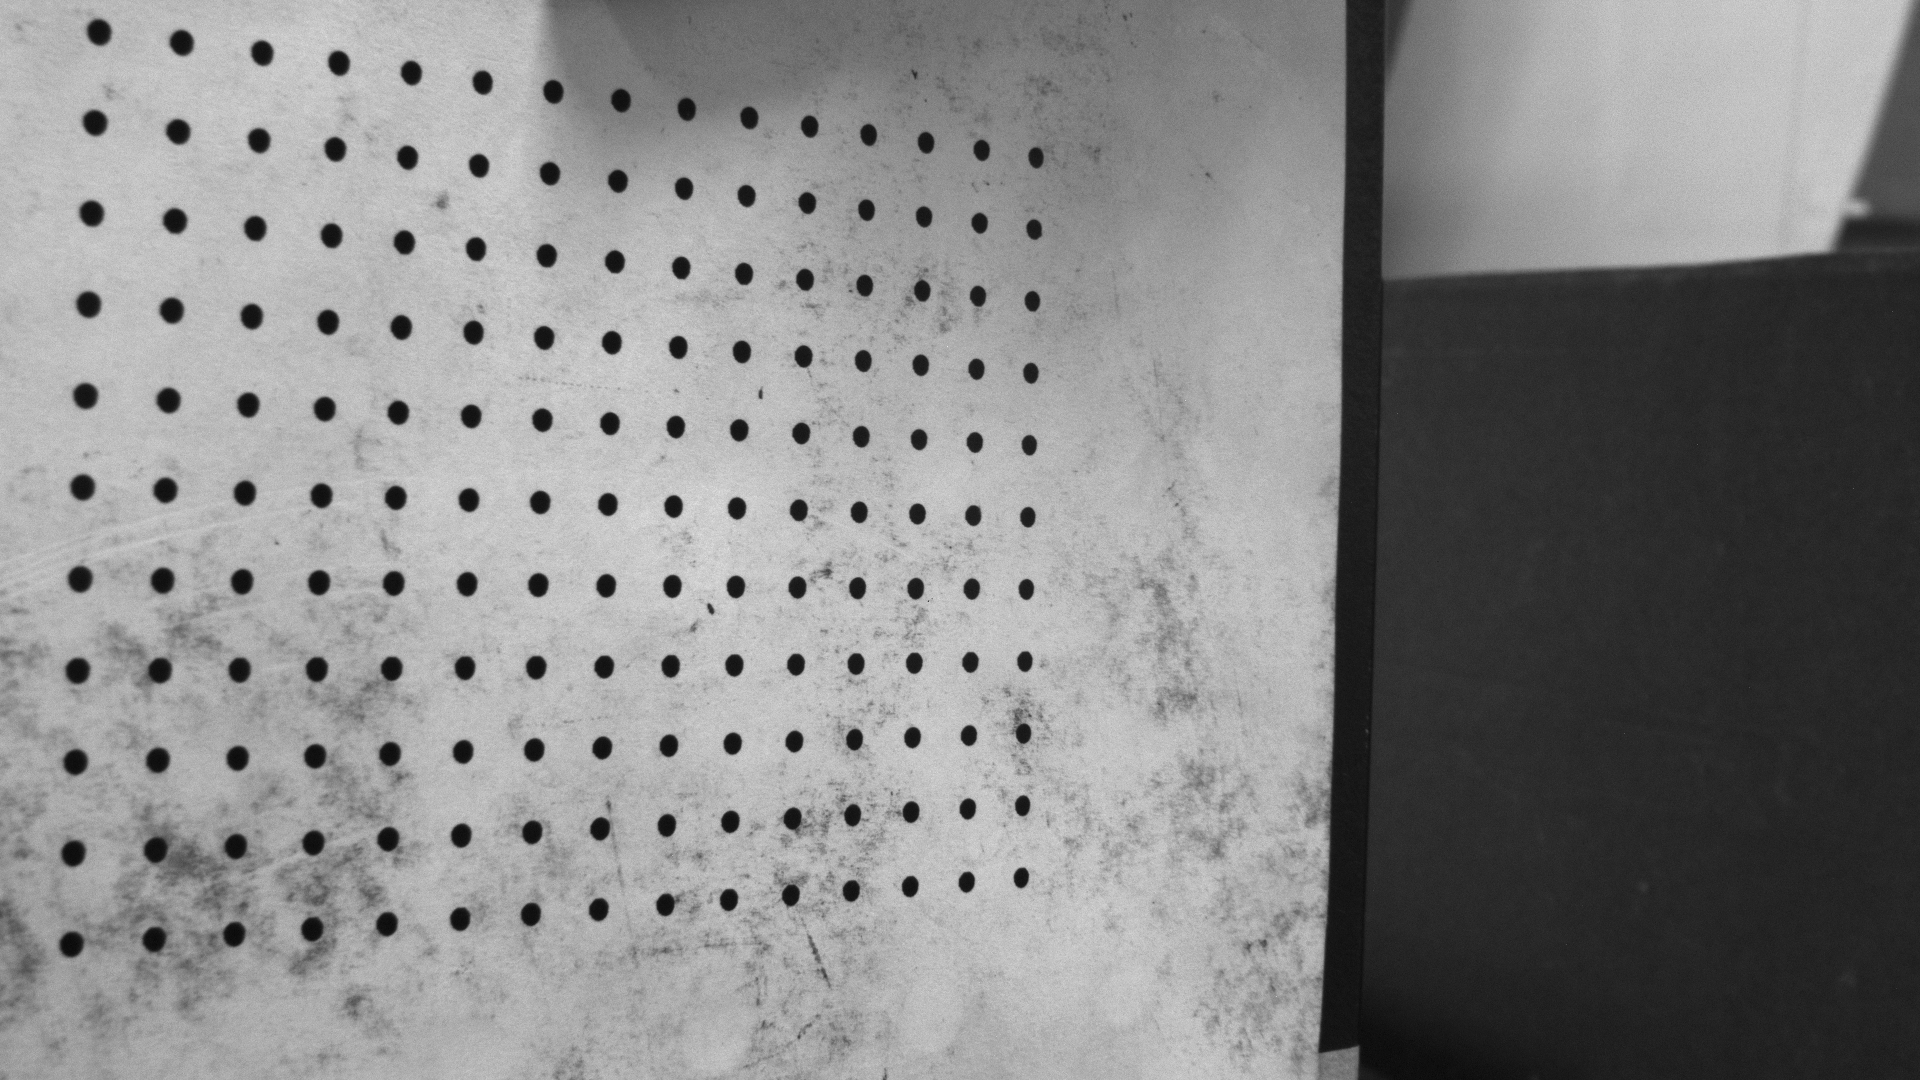
\includegraphics[width=0.52\linewidth]{scans/calibration_stereo/GE1910/20141105161936}
        }
       \subfloat{
            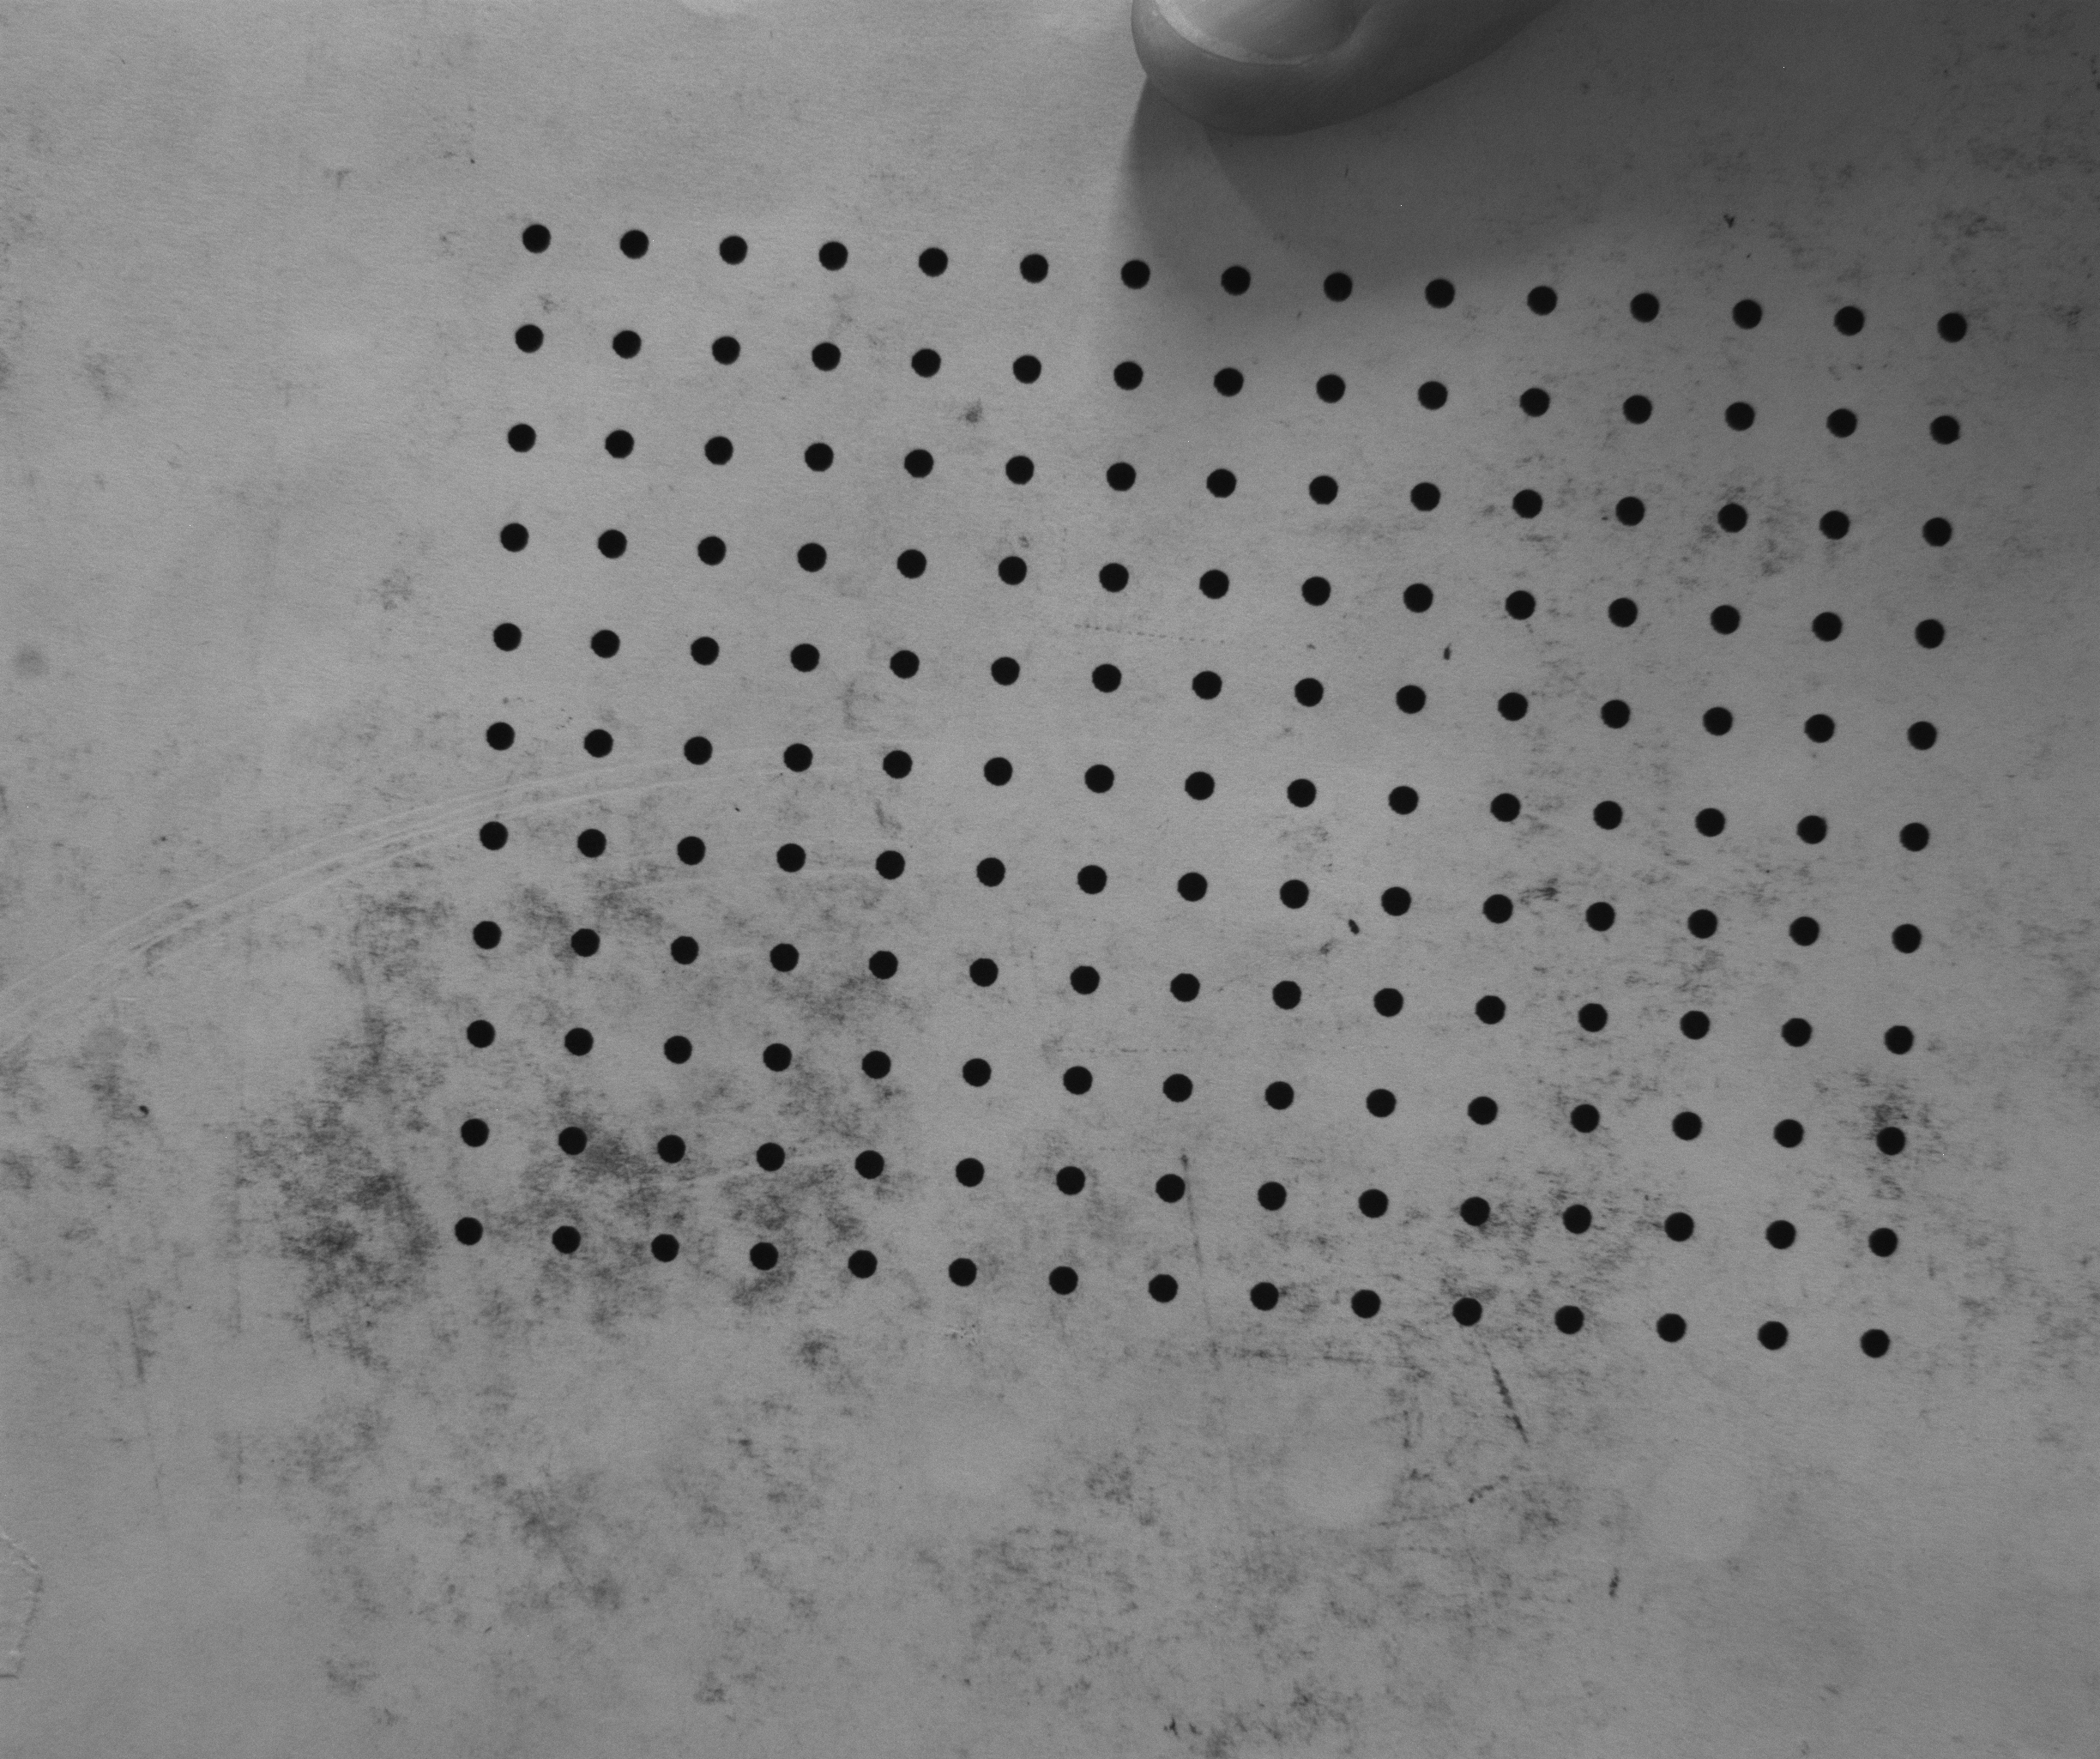
\includegraphics[width=0.35\linewidth]{scans/calibration_stereo/GC2450M/20141105161936}
        }
%        \caption{Imagenes para la calibración extrínseca entre cámaras. Izquierda: cámara 1, derecha: cámara 2}
%        \label{fig:stereoCalibrationImages1}
%\end{figure}
%
%\begin{figure}[!bth]
%    \myfloatalign
        \\
        \subfloat{
            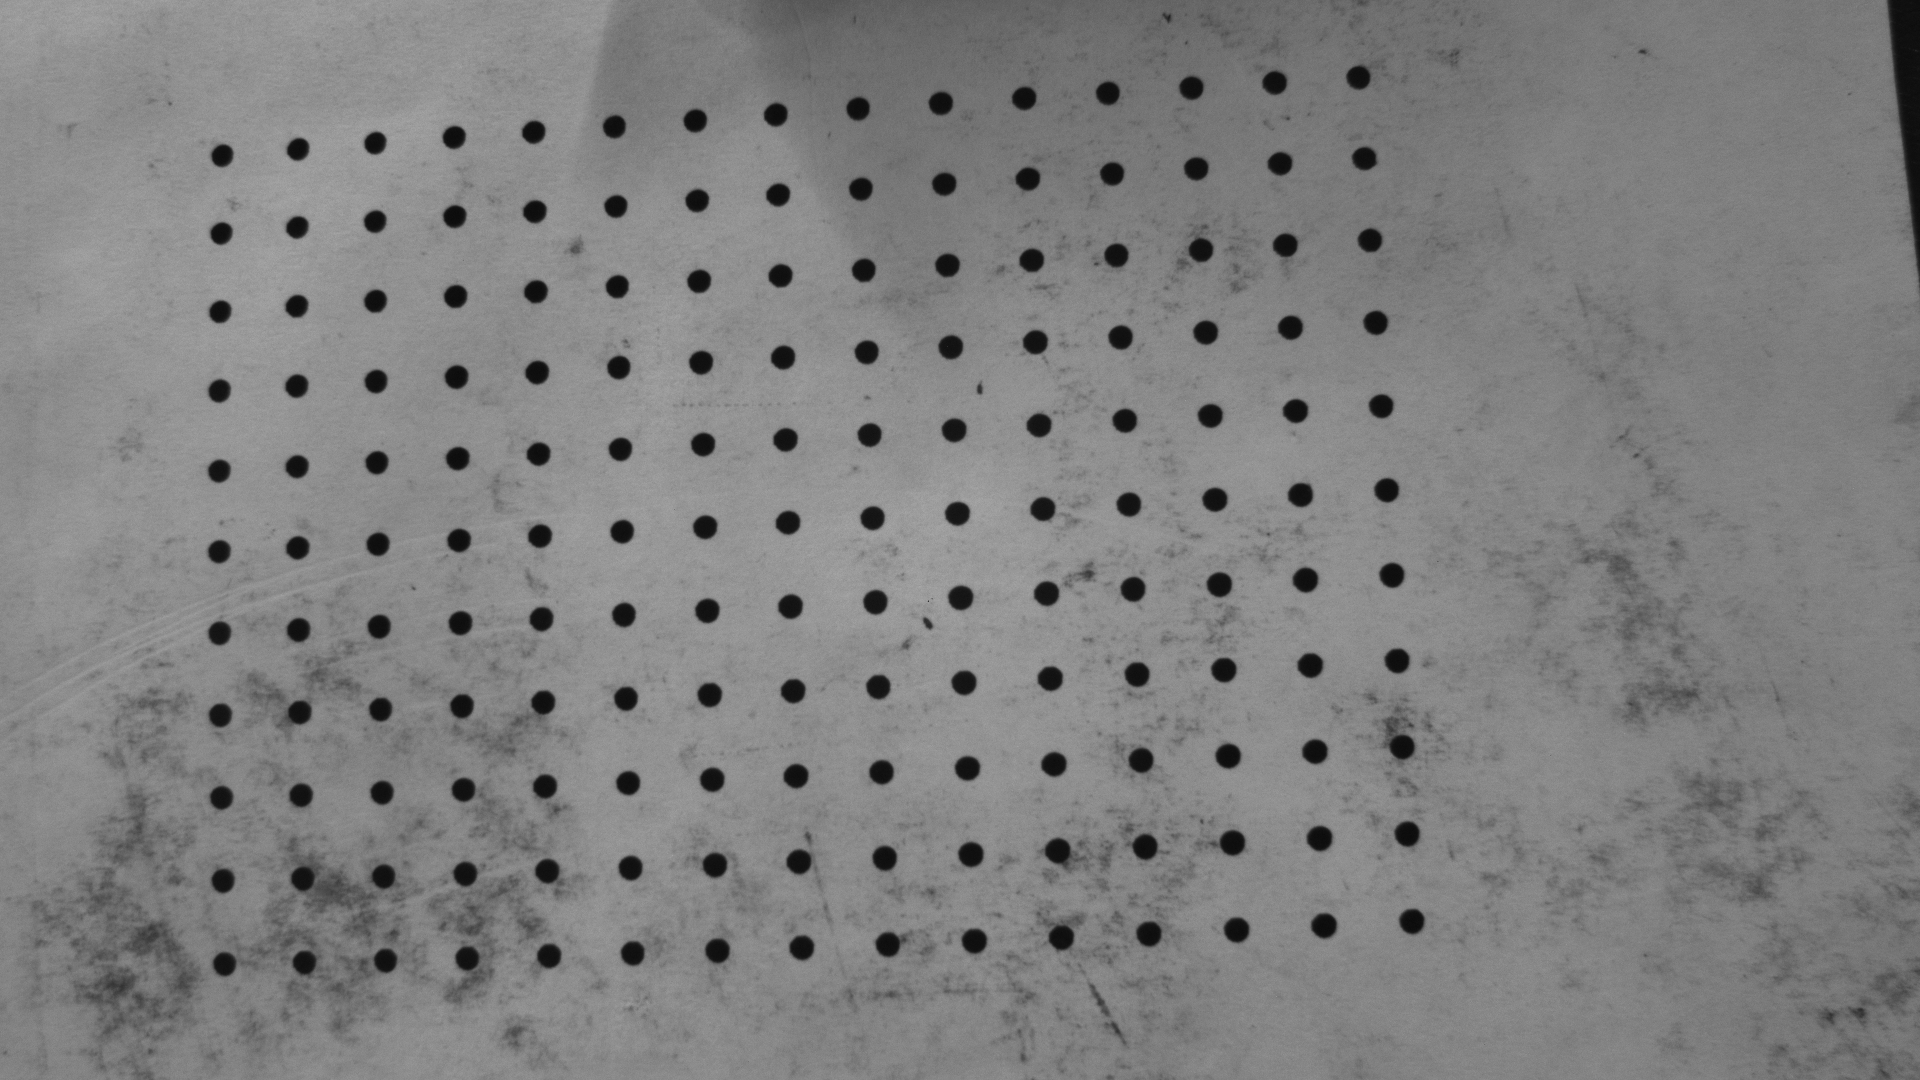
\includegraphics[width=0.52\linewidth]{scans/calibration_stereo/GE1910/20141105161953}
        }
       \subfloat{
            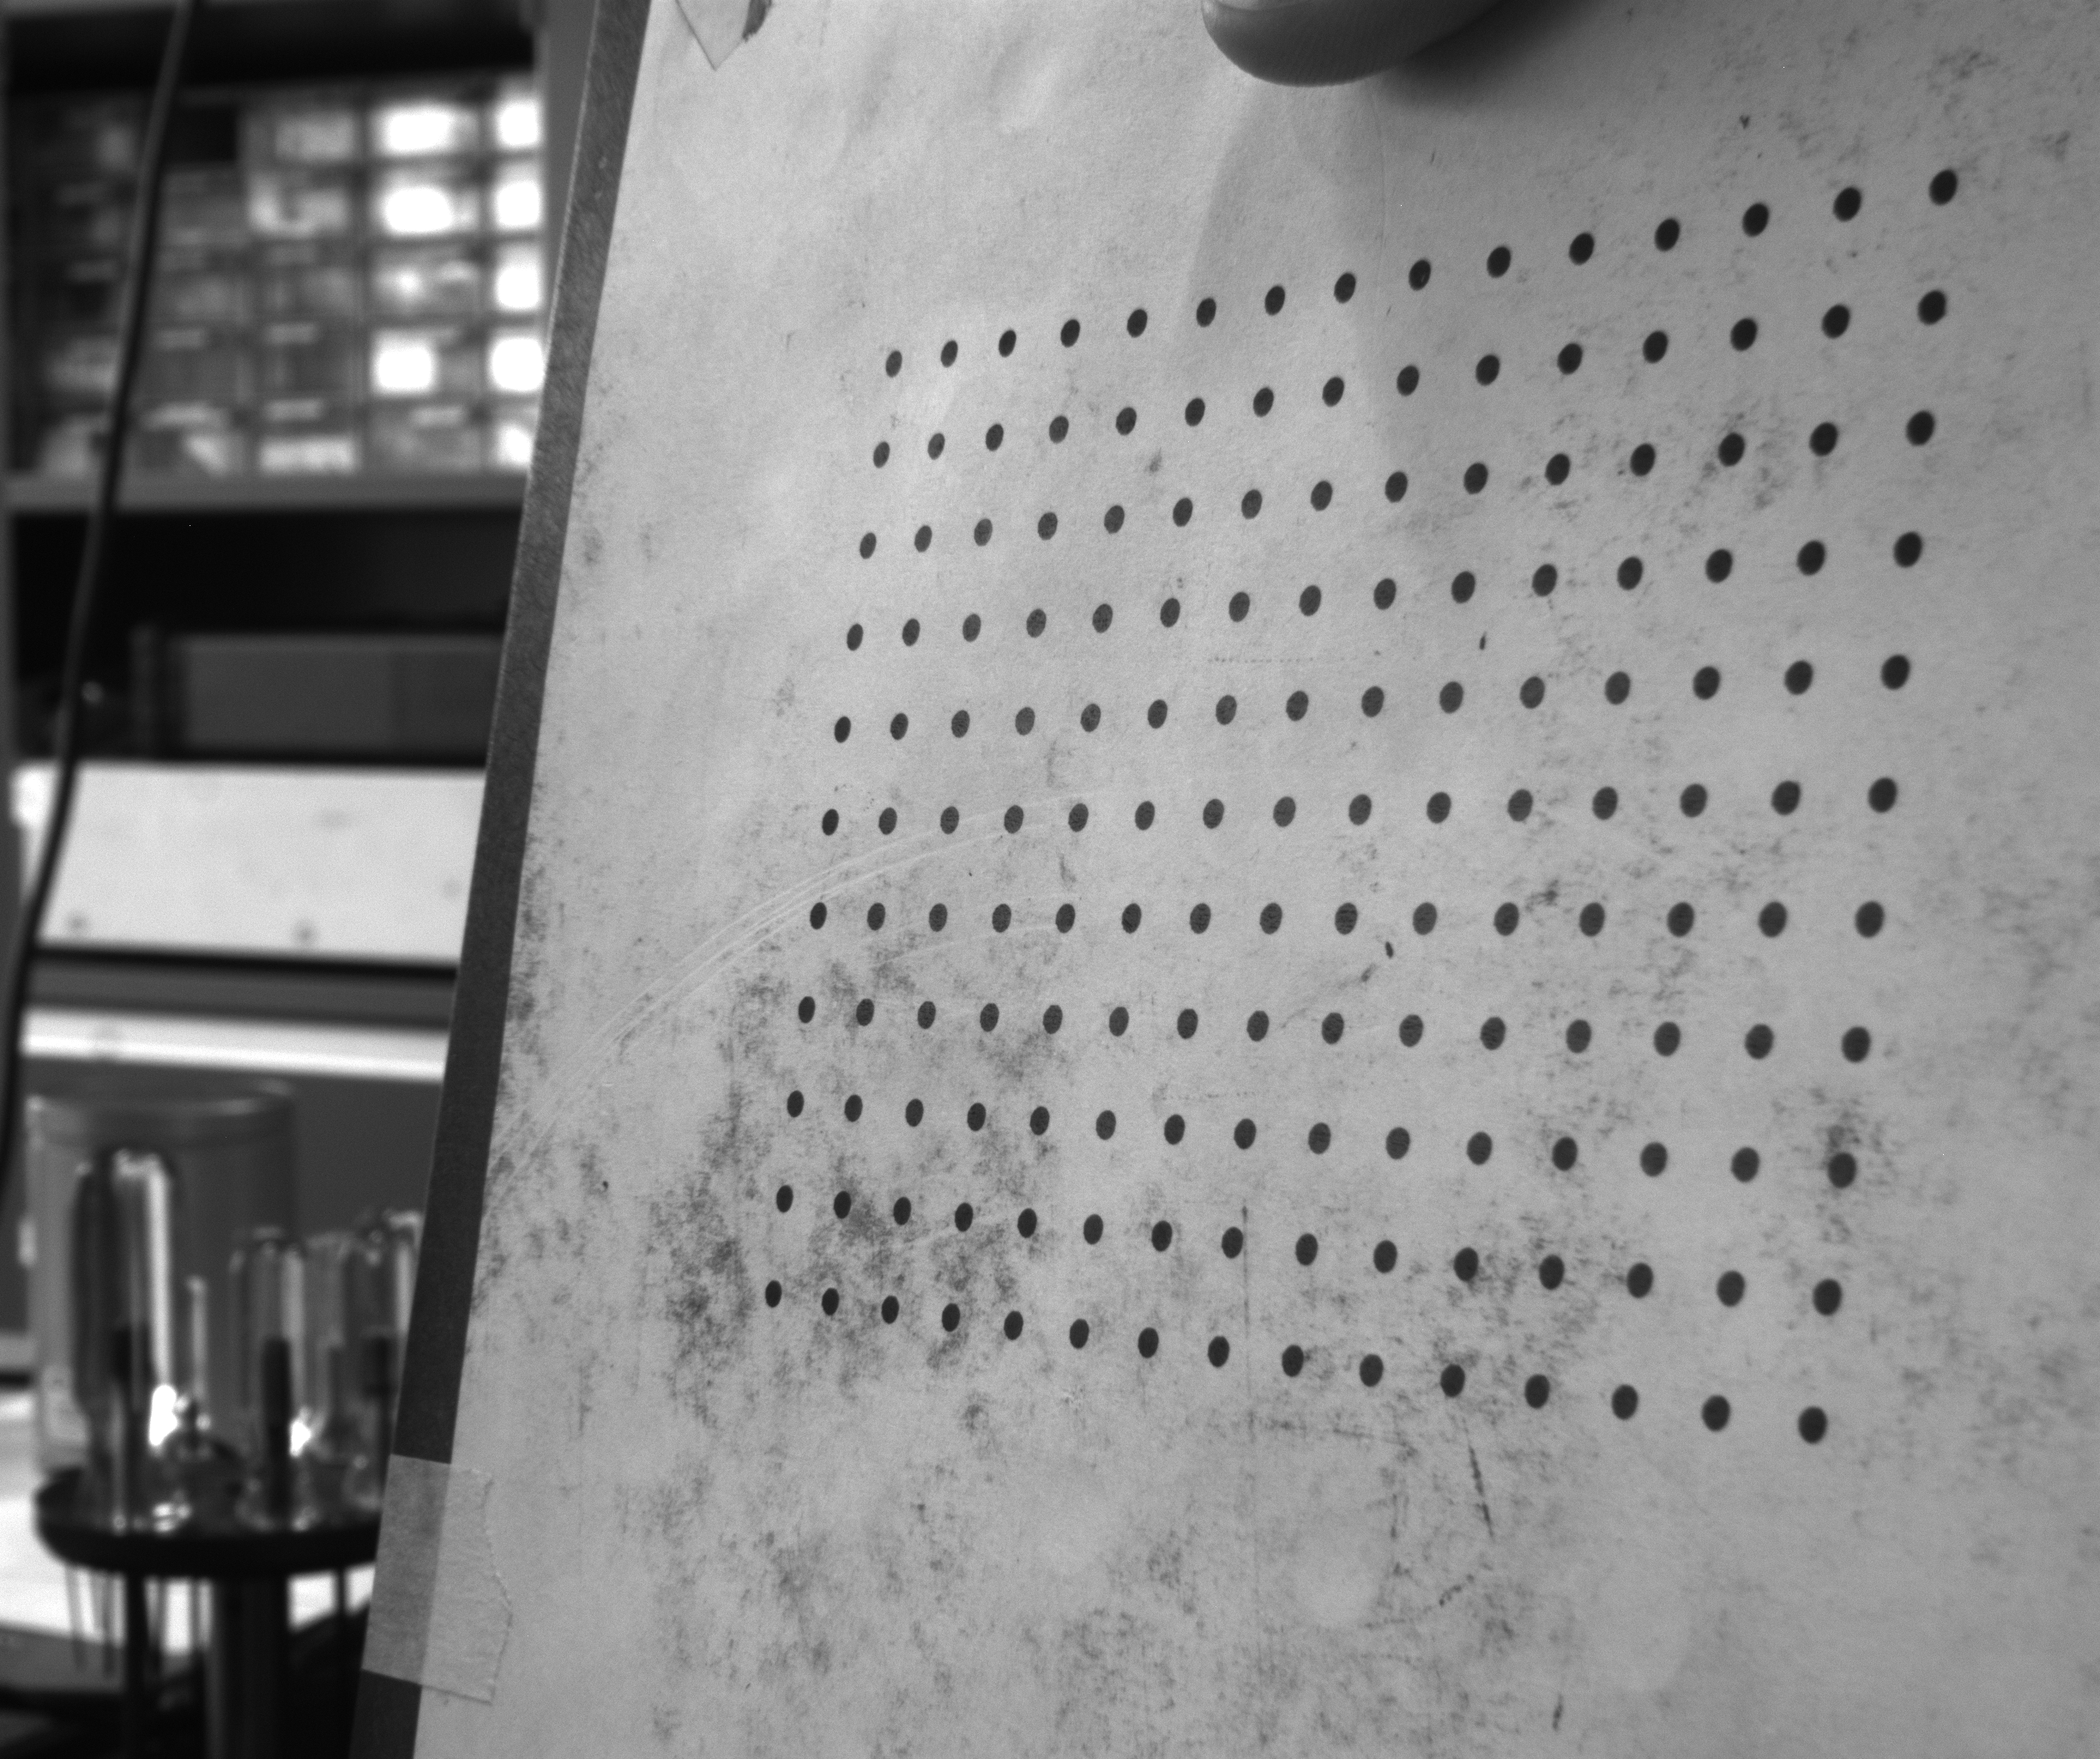
\includegraphics[width=0.35\linewidth]{scans/calibration_stereo/GC2450M/20141105161953}
        }
       \\
        \subfloat{
            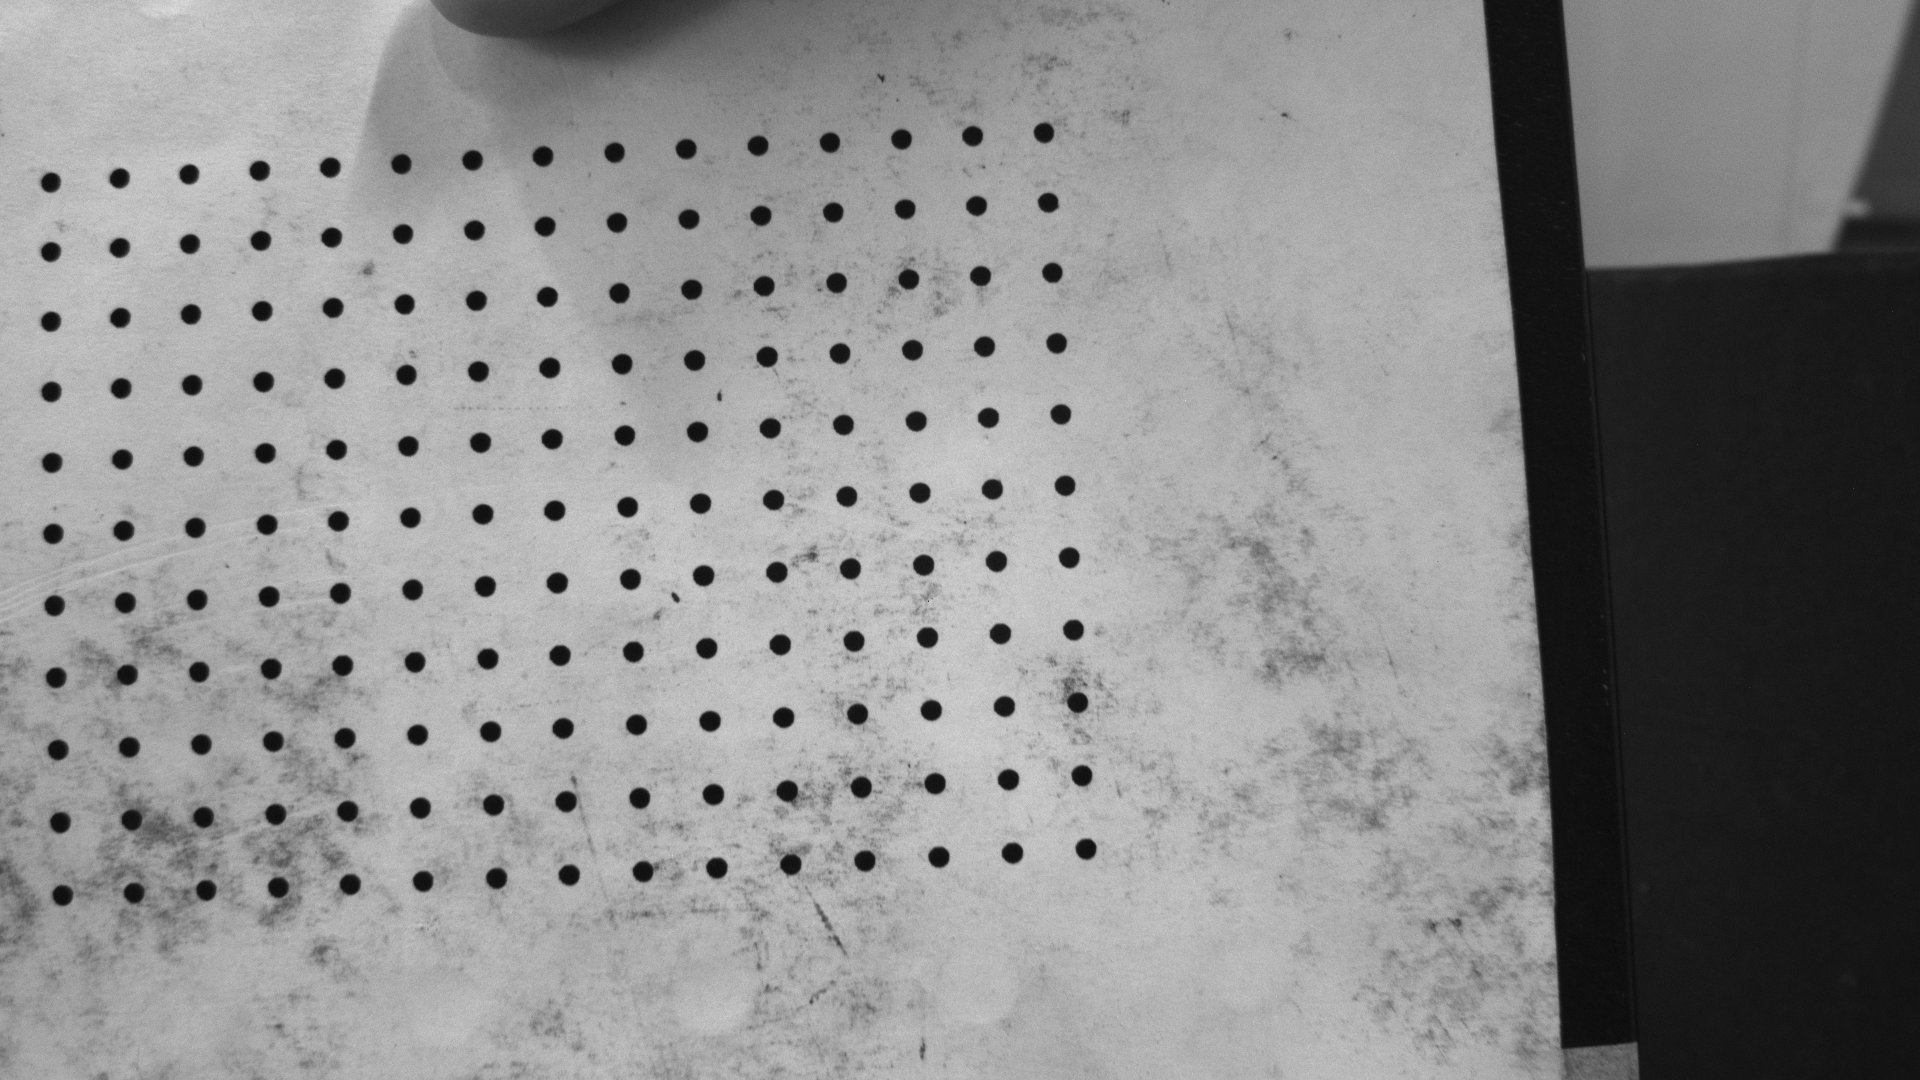
\includegraphics[width=0.52\linewidth]{scans/calibration_stereo/GE1910/20141105162029}
        }
       \subfloat{
            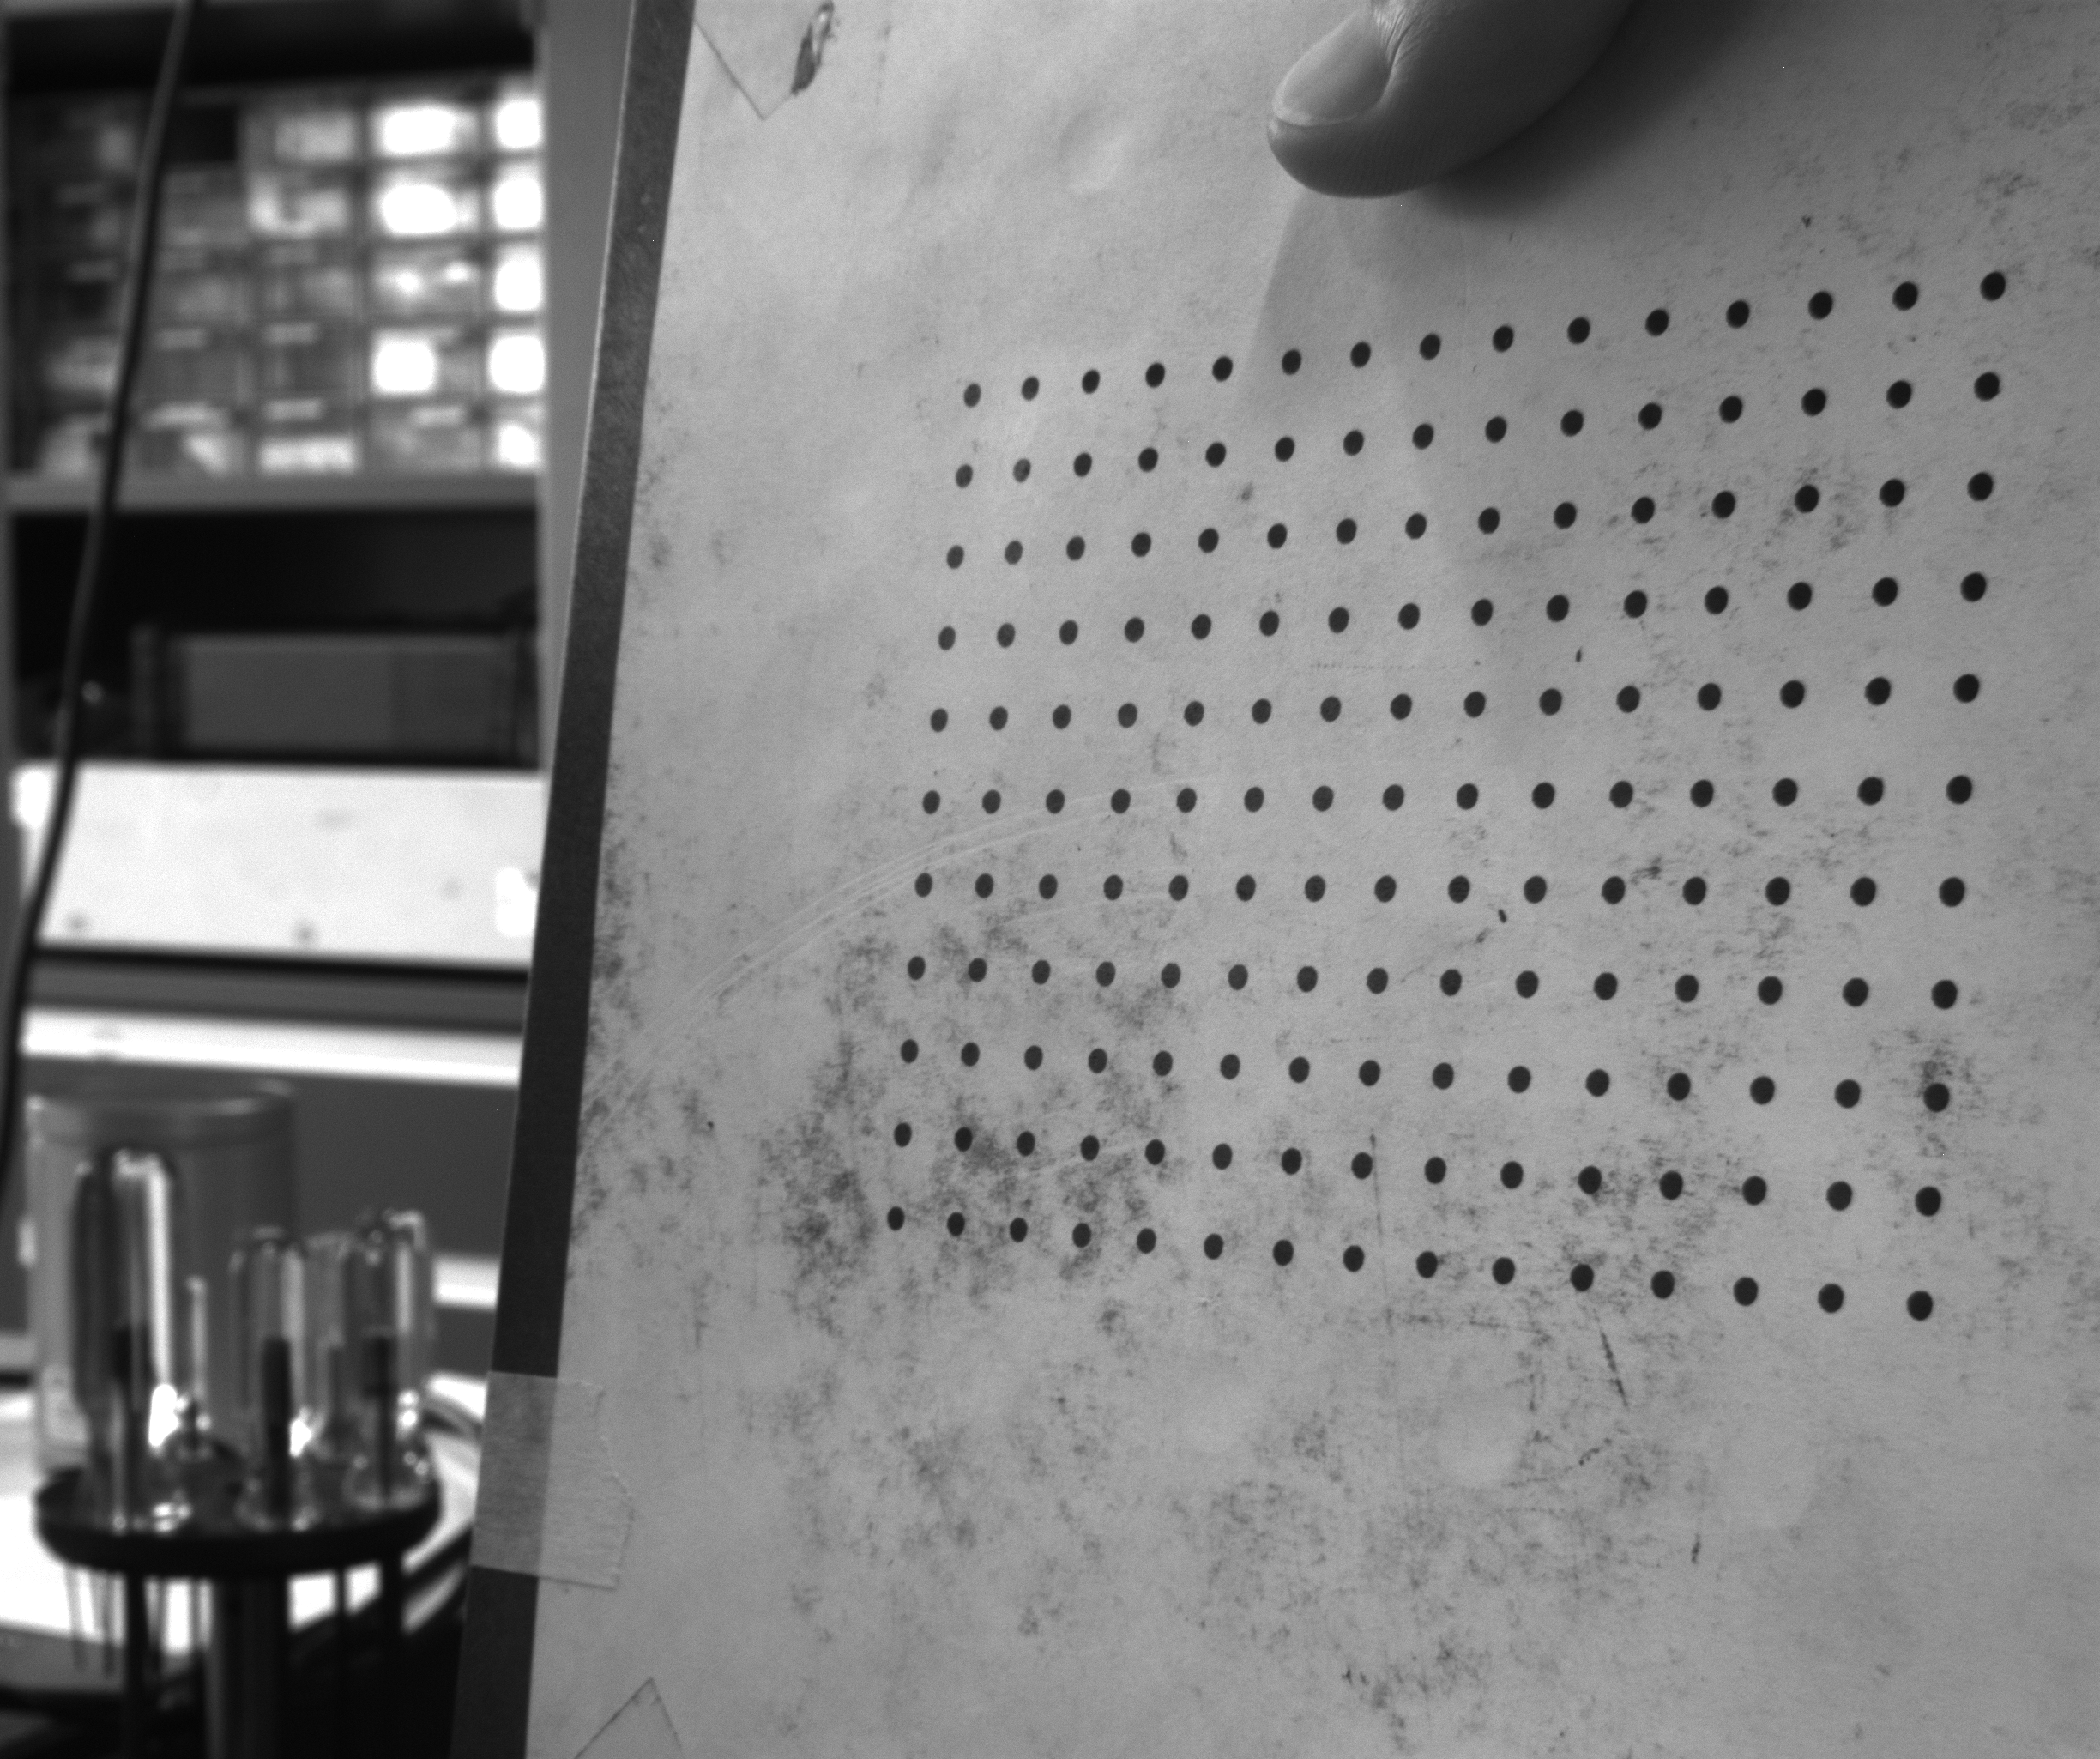
\includegraphics[width=0.35\linewidth]{scans/calibration_stereo/GC2450M/20141105162029}
        }
       \\
        \subfloat{
            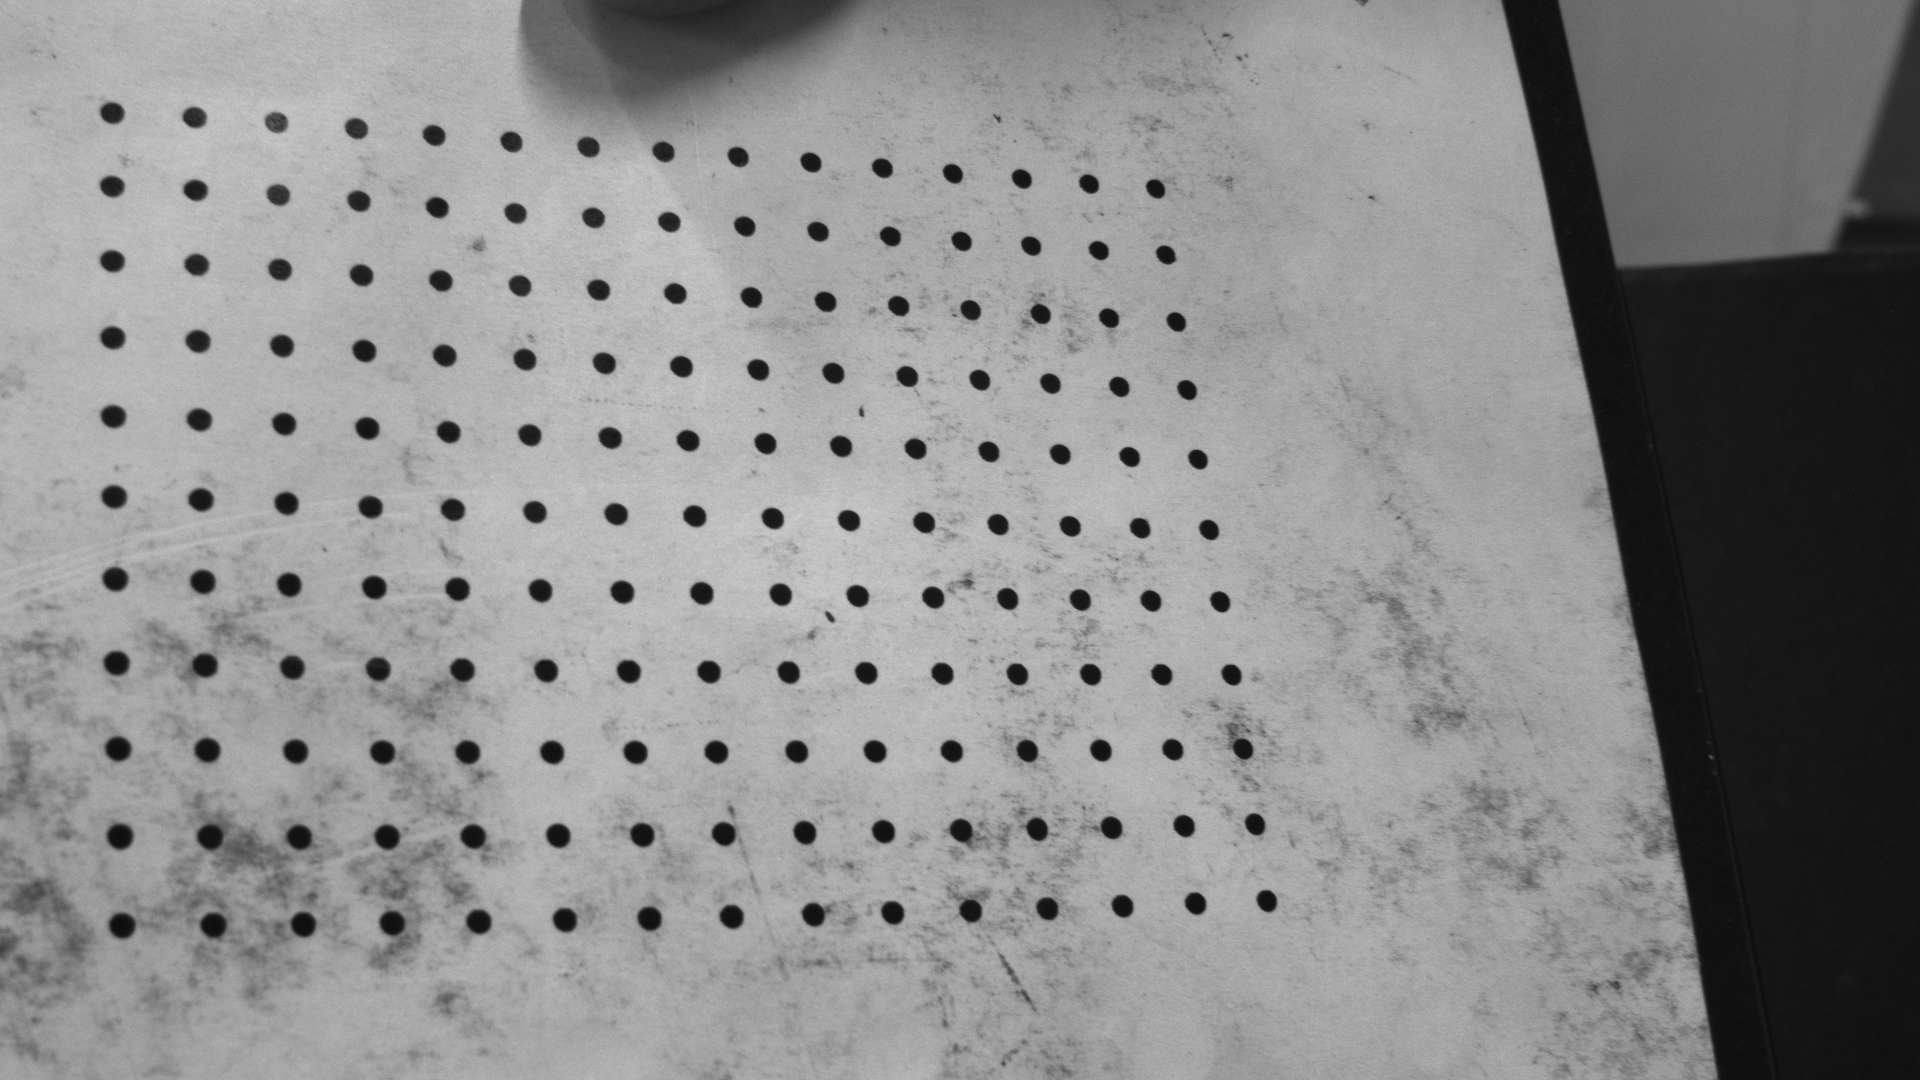
\includegraphics[width=0.52\linewidth]{scans/calibration_stereo/GE1910/20141105162046}
        }
       \subfloat{
            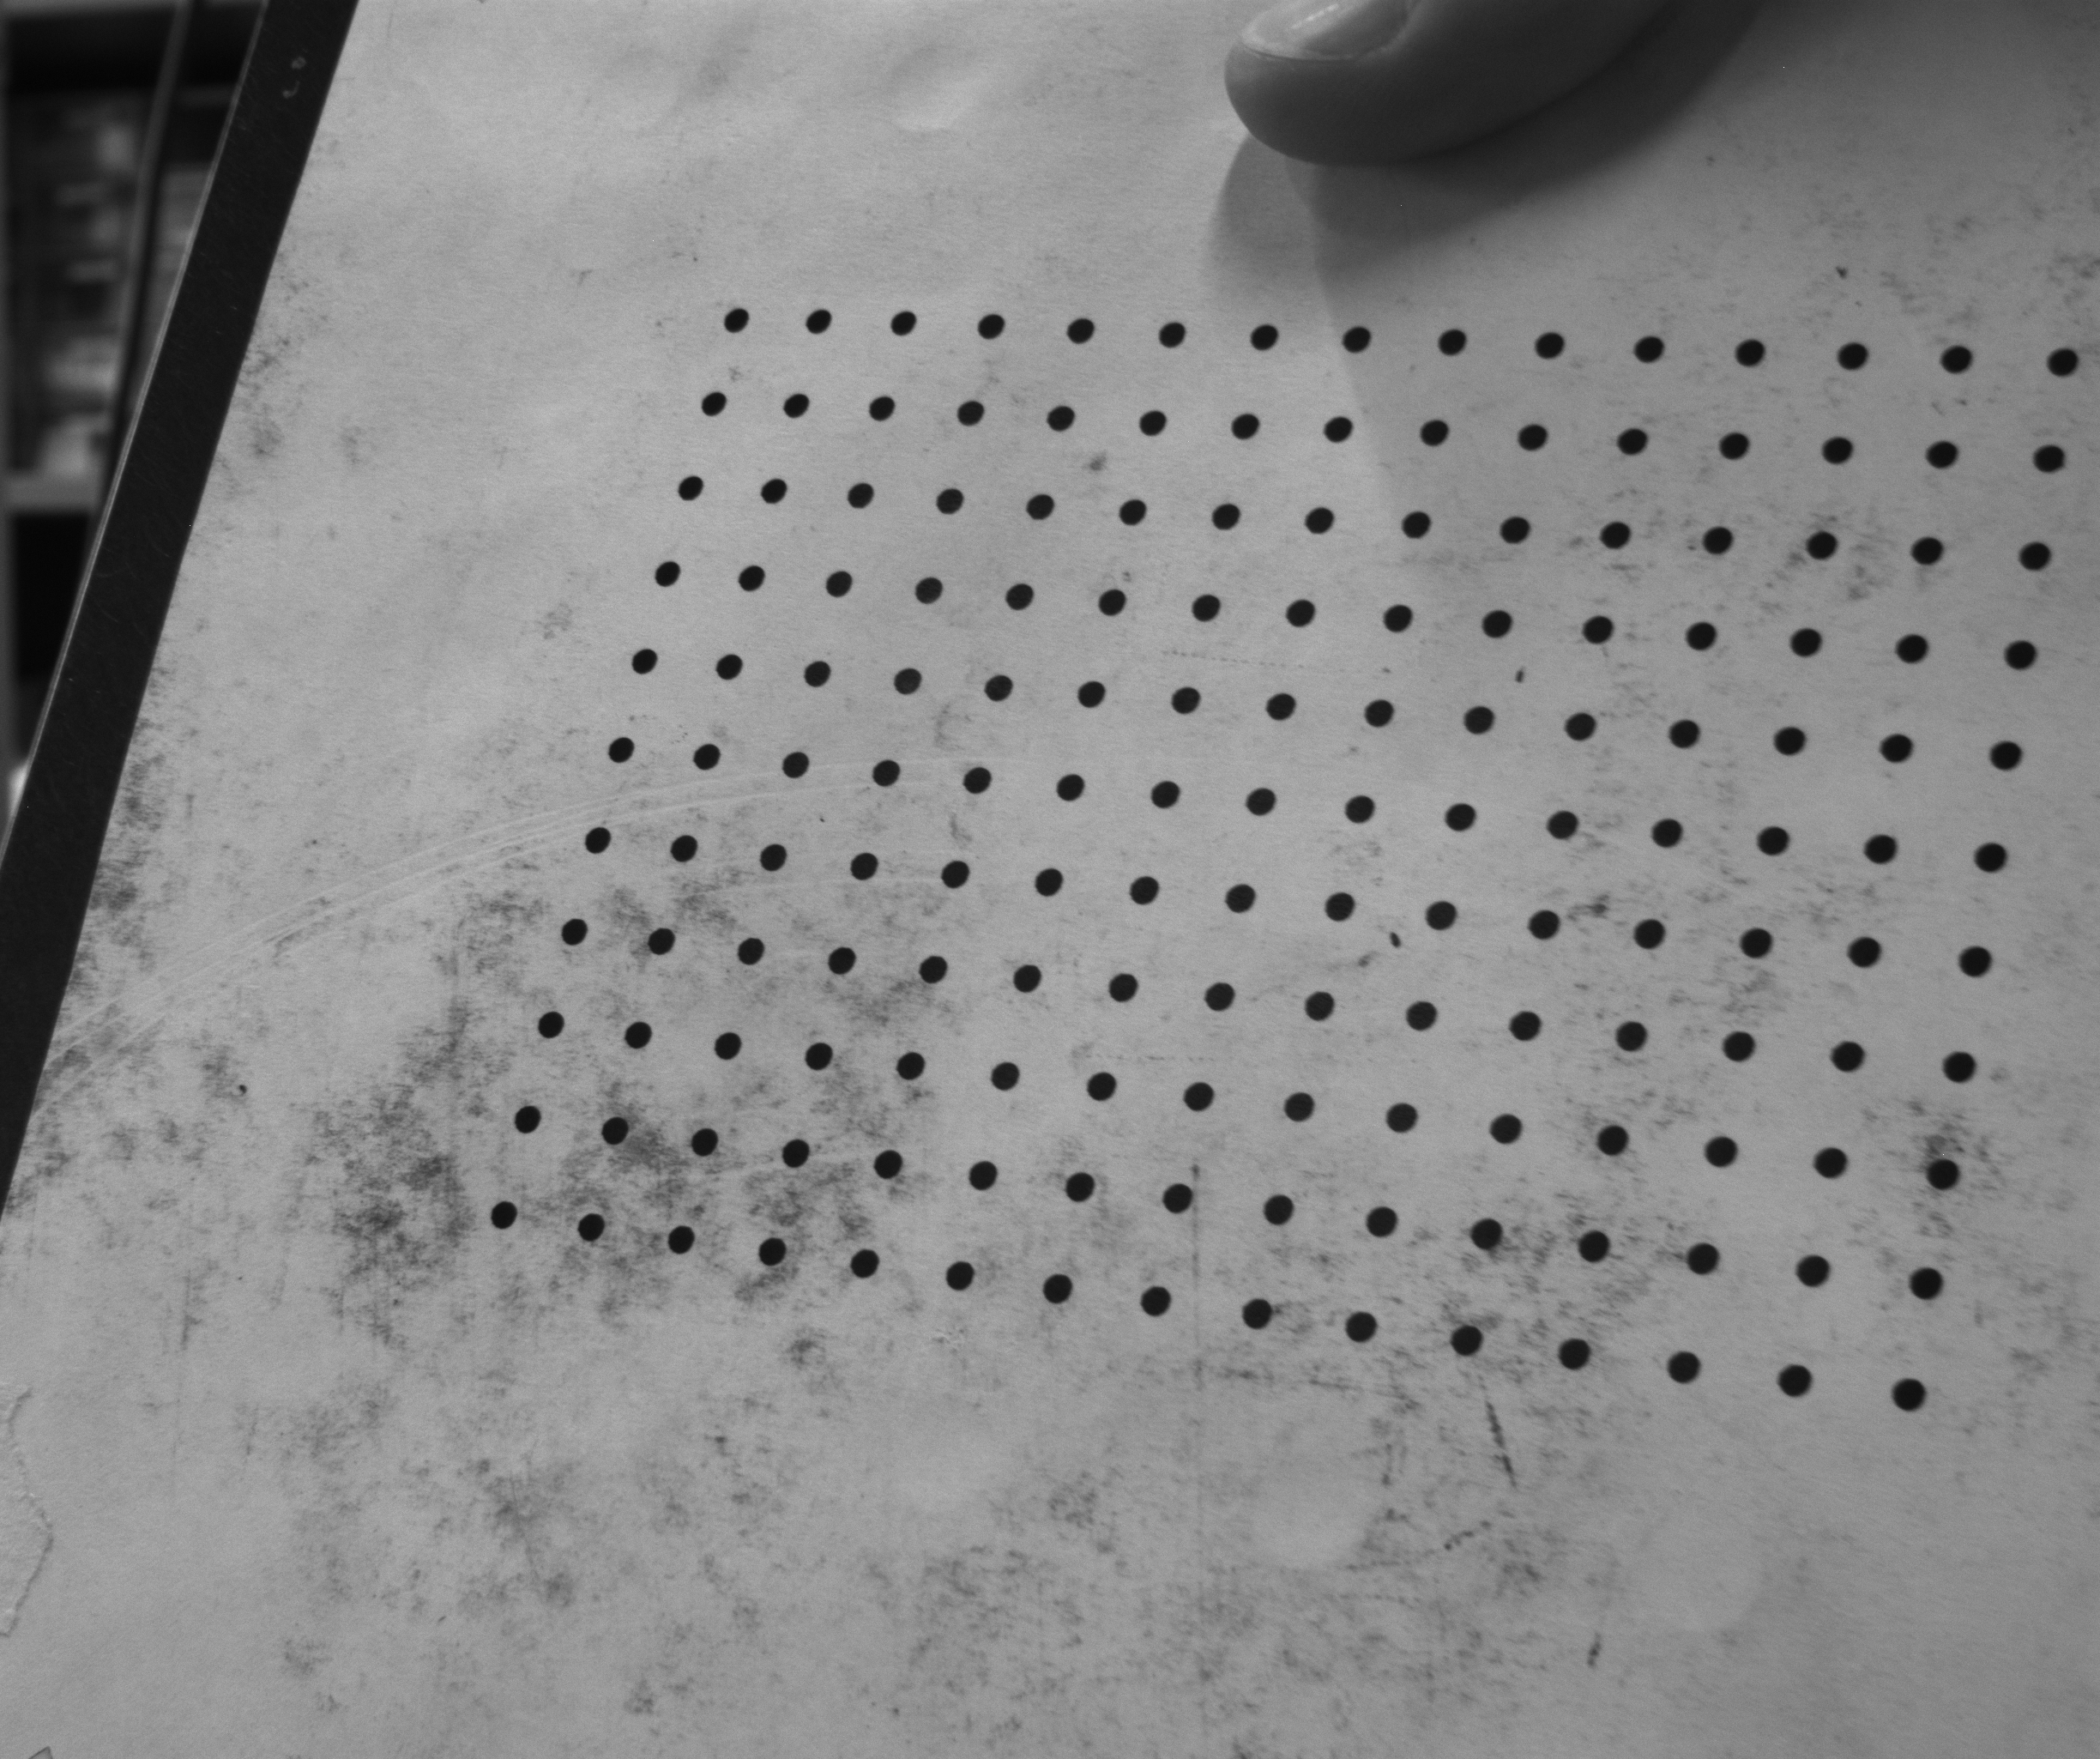
\includegraphics[width=0.35\linewidth]{scans/calibration_stereo/GC2450M/20141105162046}
        }
        \caption{Imagenes para la calibración extrínseca entre cámaras. Izquierda: cámara 1, derecha: cámara 2}
        \label{fig:stereoCalibrationImages2}
\end{figure}

%A partir de este procedimiento de calibración se obtuvieron los siguientes parámetros:

La configuración (ubicación y orientación de las cámaras y el proyector, resolución de las cámaras, etc) y calibración del dispositivo utilizadas en las pruebas nos permite obtener una resolución (distancia entre puntos) aproximada de entre $0.2$ mm (a una distancia de $20$ cm) y $0.3$ mm (a $30$ cm). Esta corresponde a la peor resolución, la cual se observa en el eje $x$ (dirección horizontal), limitada por la cantidad de columnas de pixels del proyector (sólo 480).
%La resolución vertical es mayor (aproximadamente $0.1$ mm), limitada por la cámara de menor resolución ($1080$ pixels de alto).

En estas condiciones la nube de puntos obtenida tiene entre quinientos mil y un millón de puntos aproximadamente. El tiempo de decodificación de los patrones de luz estructurada es de alrededor de medio segundo y el cálculo de la nube de puntos se lleva a cabo en menos de un segundo. Estos tiempos corresponden a la ejecución del software en una laptop actual.

\section{Objetos de prueba}
El objetivo de las pruebas es verificar el correcto funcionamiento del dispositivo y del procedimiento de calibración, y nos permitirán obtener una estimación del error. Para facilitar esta tarea se utilizarán dos tipos de objetos simples: un objeto con una superficie plana y un objeto cilíndrico. 

El objeto que utilizaremos como superificie plana es de muy alta precisión\footnote{Patrón de planicidad marca Solesa \url{http://www.solesa.com.ar/}} y presenta una superficie un tanto brillosa de color gris oscuro, similar al mármol. La superficie oscura no es la óptima para un método de medición óptico pero la reflexión resulta suficiente para permitir su utilización. Este objeto nos permitirá evaluar facilmente si estamos compensando correctamente la distorsión de los lentes. 

El objeto cilíndrico es una cupla\footnote{Una cupla es un tubo que tiene rosca por dentro y sirve para unir dos tubos} pintada de color rojo que presenta una superficie relativamente opaca. Este objeto nos permitirá evaluar la calibración completa del dispositivo, los parámetros intrínsecos y extrínsecos funcionando en conjunto. 

\section{Resultados}
Ambos objetos fueron escaneados en distintas posiciones dentro del rango de medición para observar el comportamiento del error respecto a la distancia de medición. Los resultados presentados en esta sección fueron obtenidos sin ningún tipo de filtrado ni post-procesamiento aplicado a la nube de puntos. 

\subsection{Objeto plano}
La superficie plana fue ubicada en diversas posiciones a diversas distancias respecto al dispositivo de medición. Si bien el desplazamiento no es aleatorio, tampoco fue controlado con precisión. En la \autoref{fig:setupPatronPlanicidad} se puede observar el objeto junto al dispositivo de medición.

\begin{figure}[!bth]
    \myfloatalign
        \subfloat{
            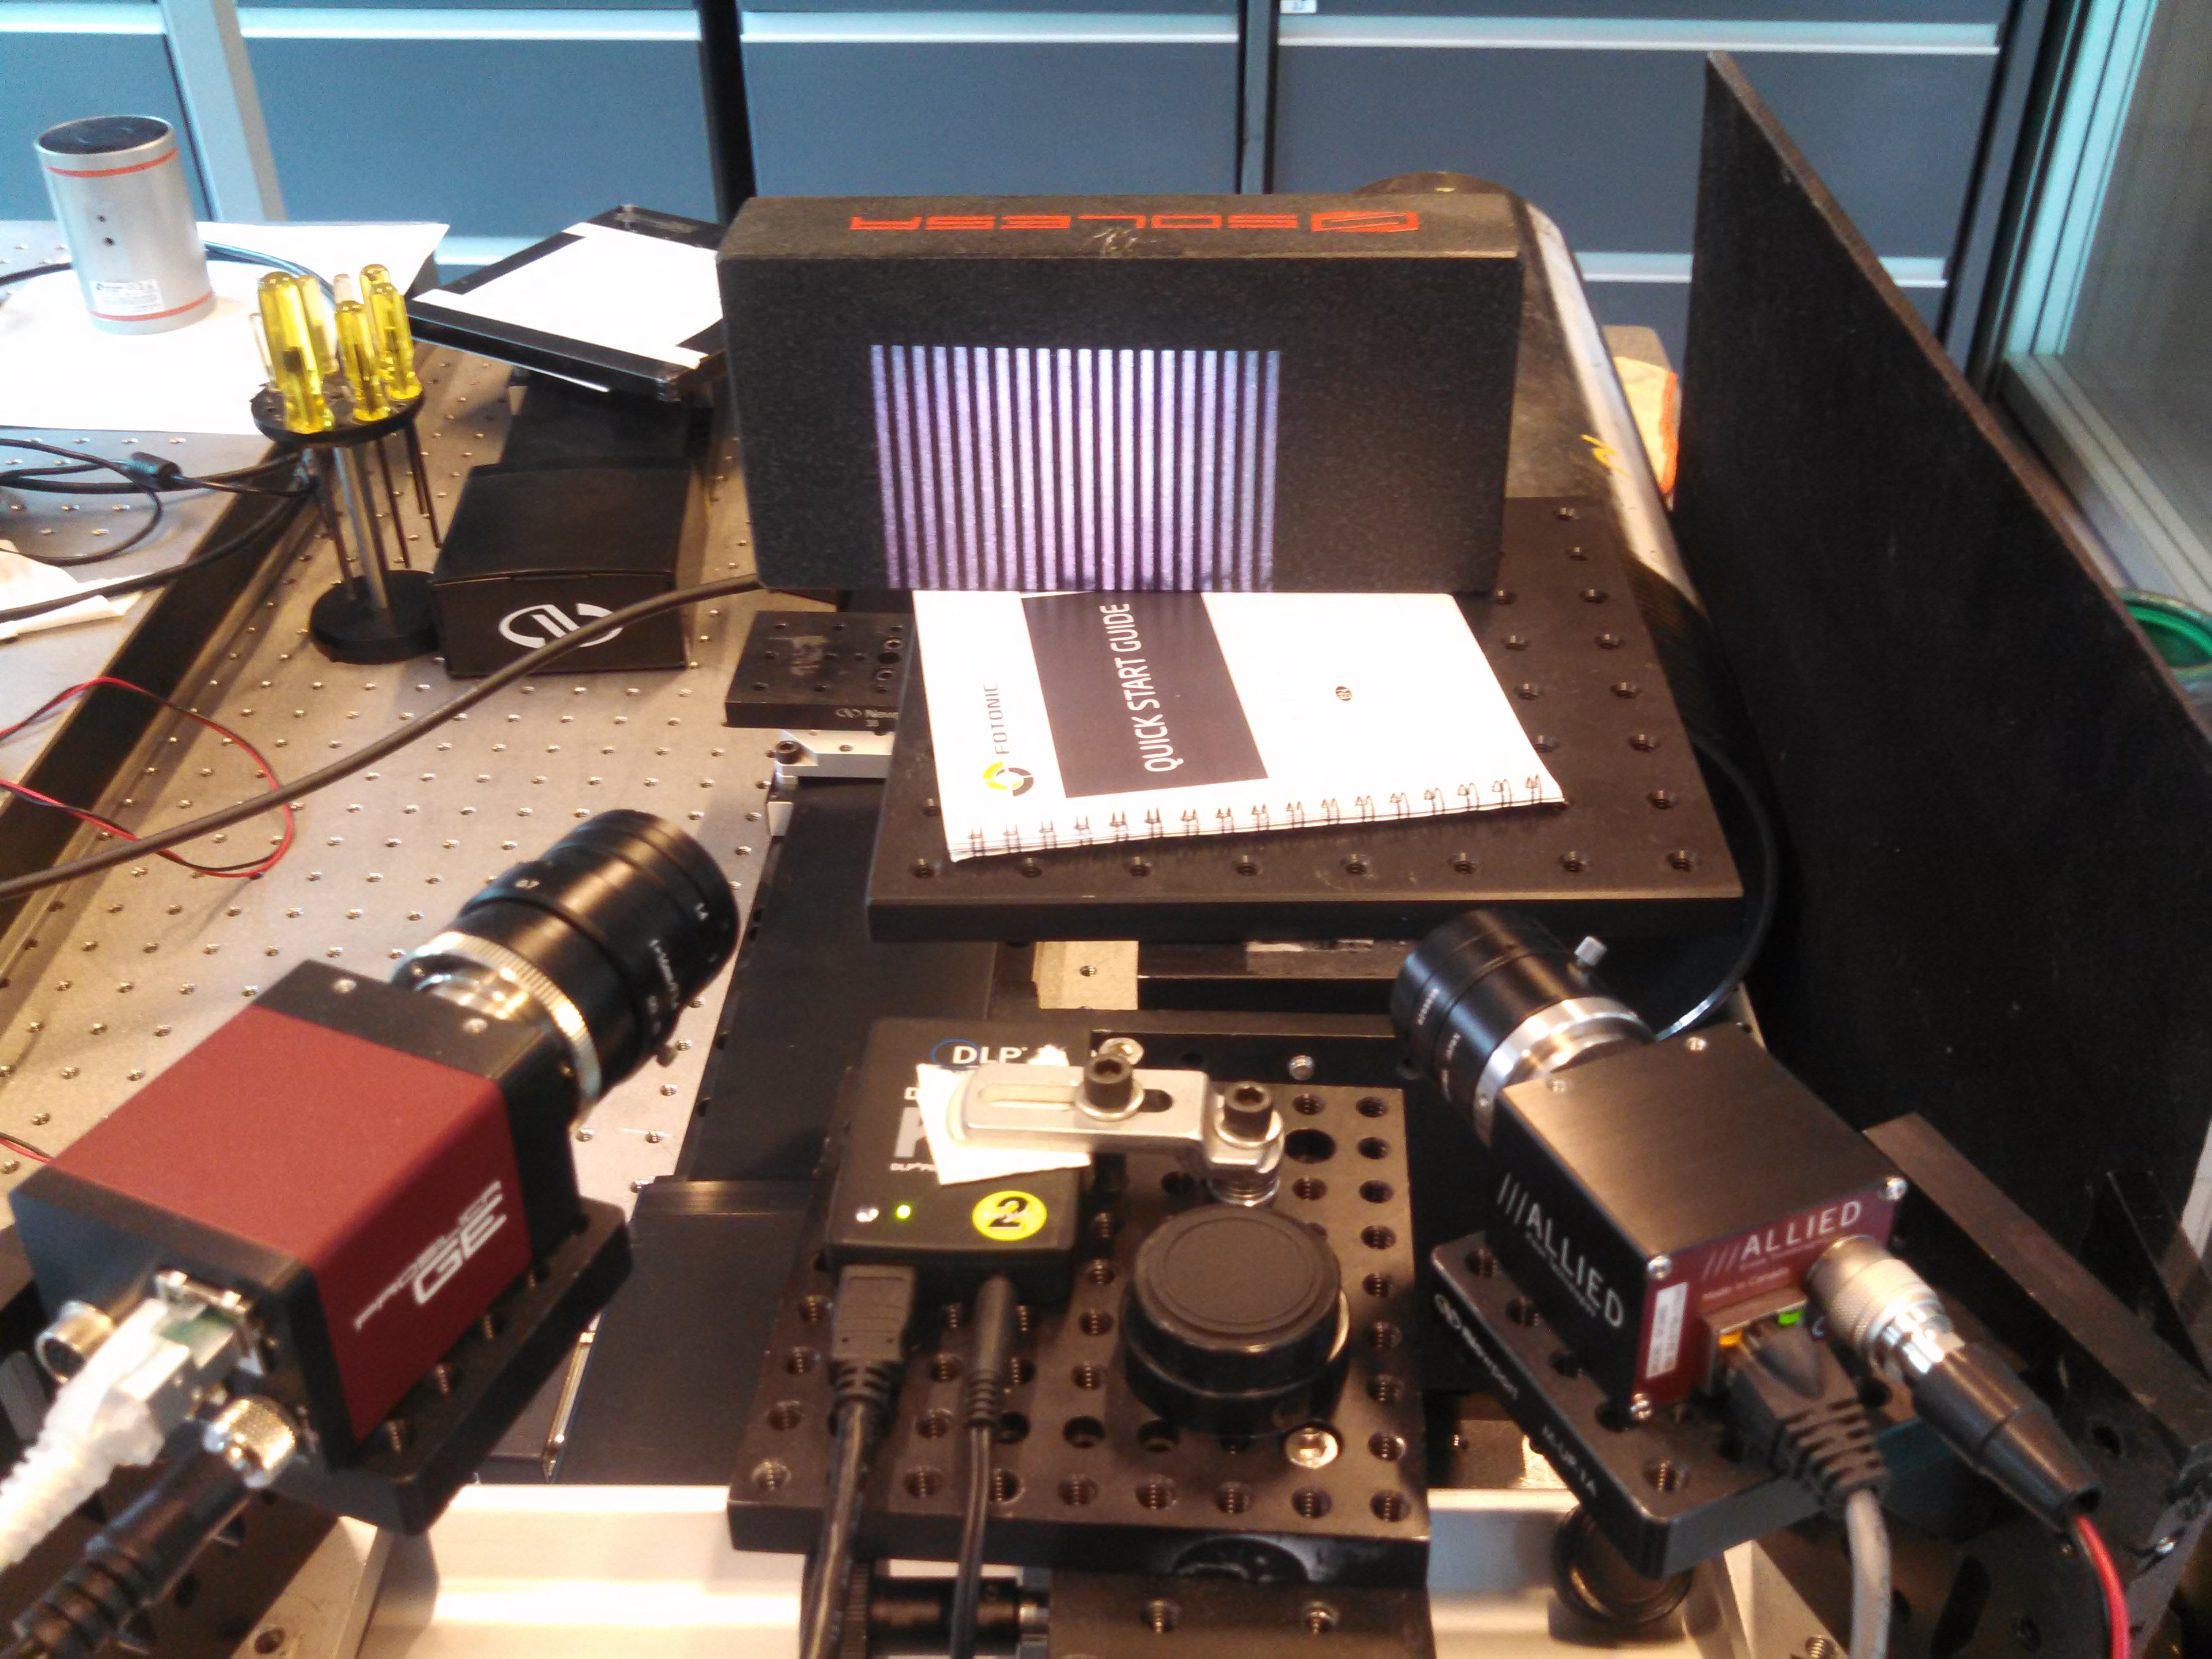
\includegraphics[width=0.49\linewidth]{images/setup/IMG_20141110_151423}
        }
        \subfloat{
            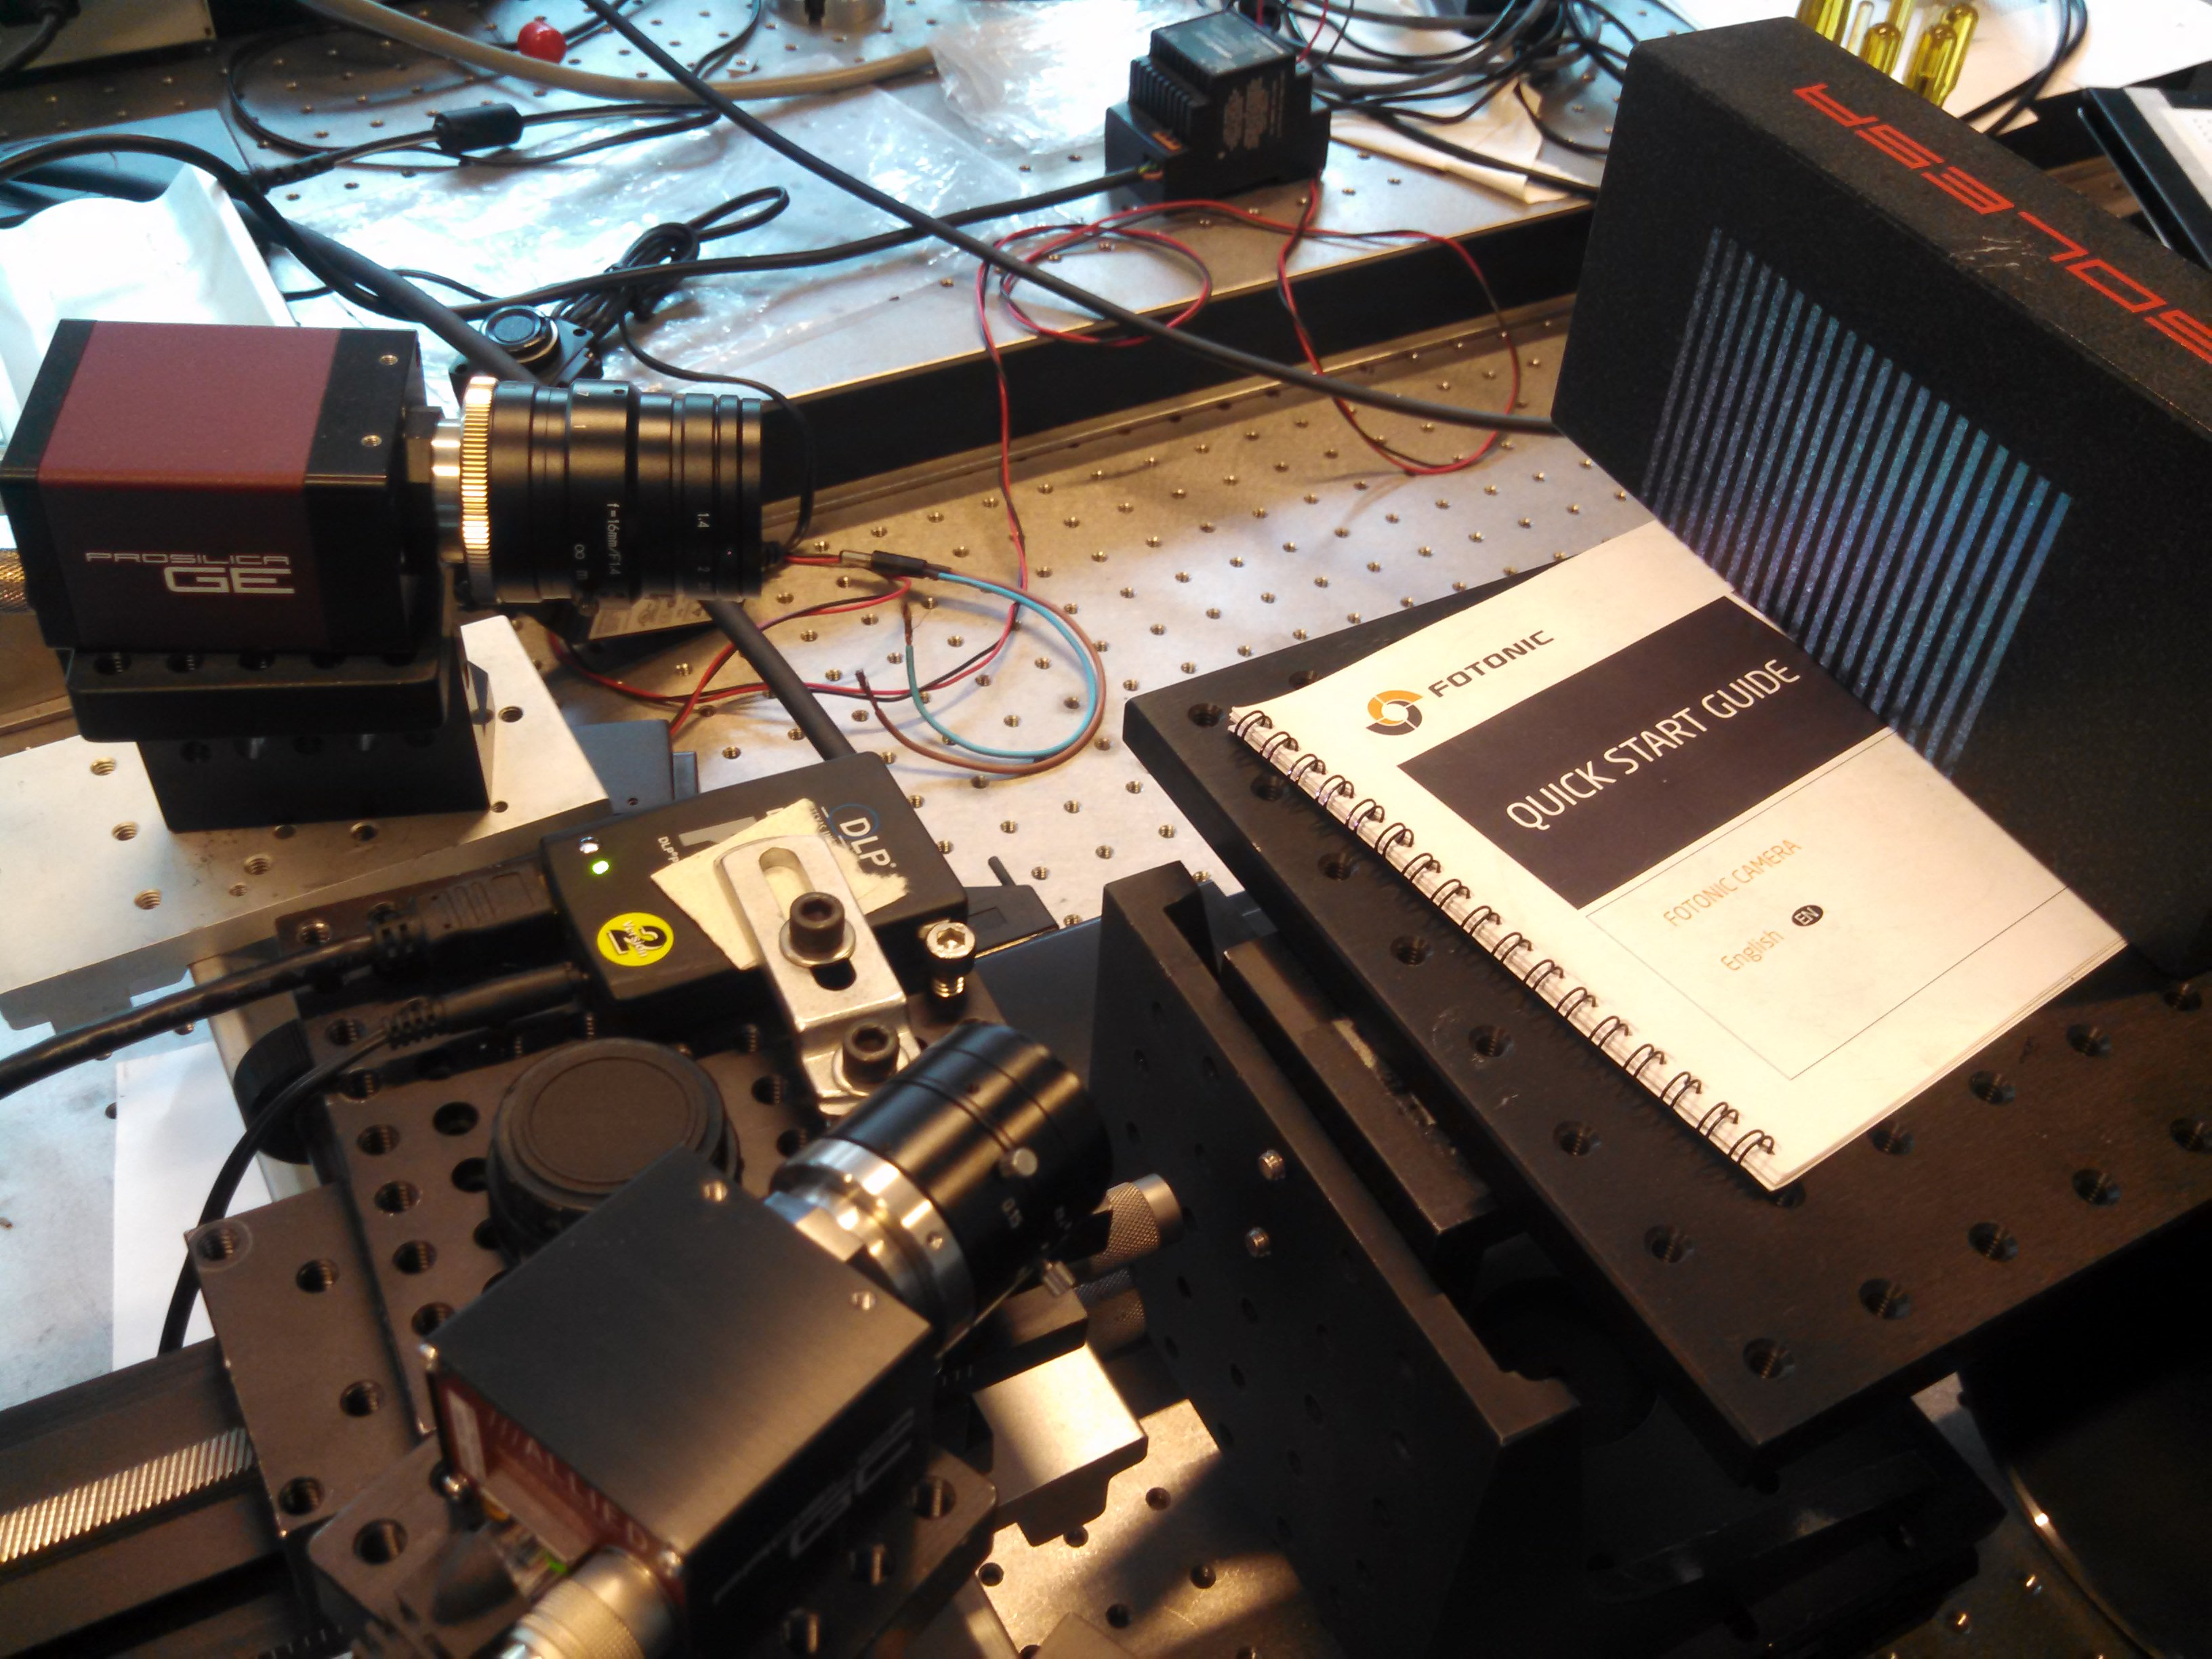
\includegraphics[width=0.49\linewidth]{images/setup/IMG_20141110_151444}
        }
        \caption{Medición del patrón de planicidad}
        \label{fig:setupPatronPlanicidad}
\end{figure}

El resultado que nos interesa obtener es la estadística del error de cada punto obtenido respecto al plano que minimiza el error. El error observado presenta una distribución gaussiana por lo que puede ser caracterizado a partir del error medio y el desvío estándar. En la \autoref{tab:patronPlanicidadResults} se pueden ver los resultados obtenidos.

\begin{table}[!bth] 
    \myfloatalign
    \begin{tabularx}{\textwidth}{ l X | c | c | c | c | c | c }
    & & \multicolumn{6}{c}{Distancia de medición [mm]} \\
    & & \rotatebox{0}{\shortstack[l]{180}} 
       & \rotatebox{0}{\shortstack[l]{200}} 
       & \rotatebox{0}{\shortstack[l]{220}} 
       & \rotatebox{0}{\shortstack[l]{240}} 
       & \rotatebox{0}{\shortstack[l]{260}} 
       & \rotatebox{0}{\shortstack[l]{290}} \\ 
    \hline
    & Error medio [um] & $4.0$ & $0.2$ & $0.6$ & $0.4$ & $0.6$ & $8.8$ \\ 
    \hline
    & Desvío estandar [um] & $77.5$ & $55.3$ & $51.2$ & $57.4$ & $65.2$ & $87.4$ \\ 
%    \hline
%    & Figura & 
%    \ref{fig:patronPlanicidadScan18cm200um} & \ref{fig:patronPlanicidadScan20cm200um} & 
%    \ref{fig:patronPlanicidadScan22cm200um} & \ref{fig:patronPlanicidadScan24cm200um} & 
%    \ref{fig:patronPlanicidadScan26cm200um} & \ref{fig:patronPlanicidadScan29cm200um} \\ 
    \hline
    \end{tabularx}
    \caption{Resultados de la medición del objeto plano}
    \label{tab:patronPlanicidadResults}
\end{table}

Lo que podemos observar es que la calibración funciona razonablemente bien, con un desvío estándar del error menor a los $0.1$mm. En la \autoref{fig:patronPlanicidadFitErrorVsDistance} se puede ver el comportamiento del desvío estándar del error respecto a la distancia.

\begin{figure}[!bth]
    \myfloatalign
        {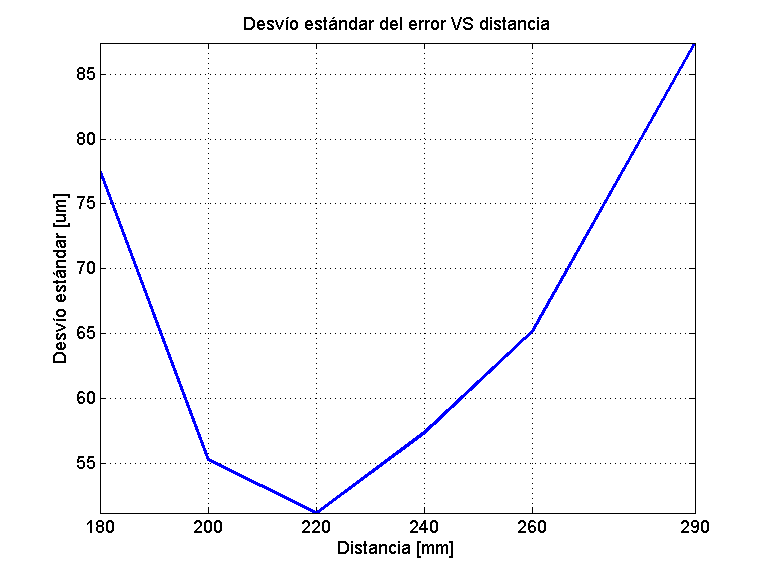
\includegraphics[width=1.0\linewidth]{scans/plotPlaneSD}}
        \caption{Objeto plano: desvío estándar del error en función de la distancia}
        \label{fig:patronPlanicidadFitErrorVsDistance}
\end{figure}

El error debería presentar un comportamiento monotónicamente creciente respecto a la distancia, sin embargo se observa que el error es alto a la menor distancia, $180$mm, y luego disminuye levemente. Las imagenes obtenidas para el plano a $180$mm no estaban bien definidas, se observan fuera de foco, lo que puede explicar este comportamiento.

La distancia de medición que presenta los mejores resultados es la zona para la cual el dispositivo fue calibrado y los lentes fueron enfocados. Luego el comportamiento del error parece adecuarse a una función cuadrática de la distancia, lo que se ajusta al error aleatorio teórico esperado para un sistema basado en triangulación \cite{khoshelham2012accuracy}.

En las figuras \ref{fig:planeScanViews1} y \ref{fig:planeScanViews2} se muestran cada una de las nubes de puntos obtenidas. El color de cada punto corresponde al error respecto al plano fiteado, y a la derecha se puede observar la escala de colores junto con un histograma. Estas imágenes fueron obtenidas con el software CloudCompare.



\begin{figure}[!bth]
    \myfloatalign
        \subfloat[Medicion del patrón de planicidad a $\approx$18cm]{
            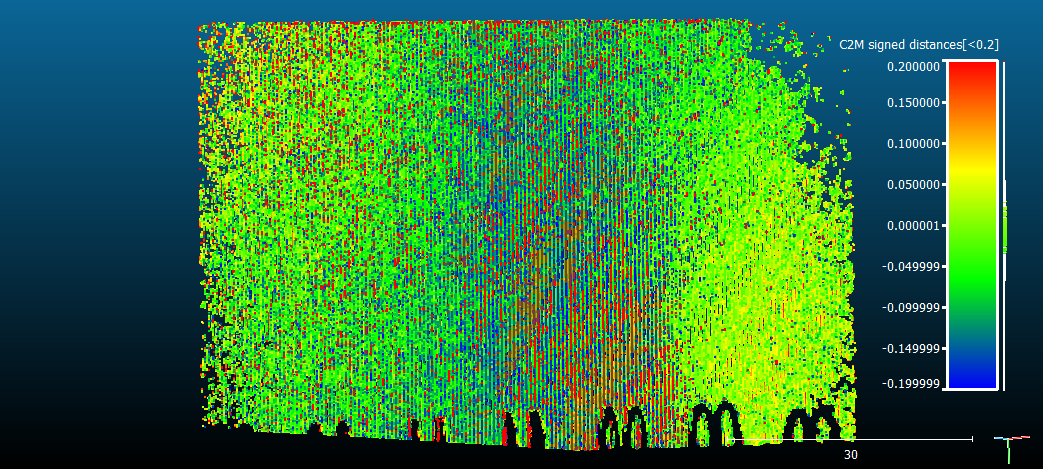
\includegraphics[width=1.0\linewidth]{scans/patronPlanicidad/2014.11.10_15.27.14/planeError_max200um}
        }
        \\
        \subfloat[Medicion del patrón de planicidad a $\approx$20cm]{
            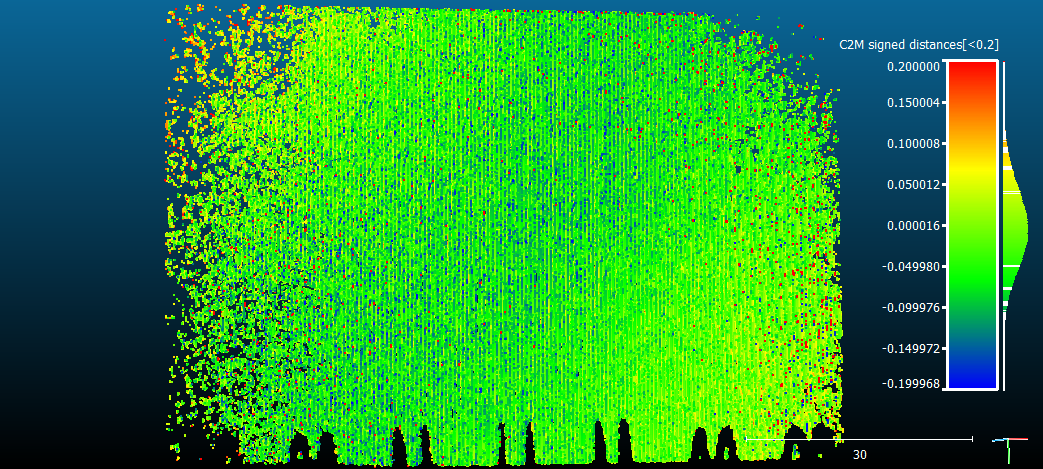
\includegraphics[width=1.0\linewidth]{scans/patronPlanicidad/2014.11.10_15.50.53/planeError_max200um}
        }
        \\
        \subfloat[Medicion del patrón de planicidad a $\approx$22cm]{
            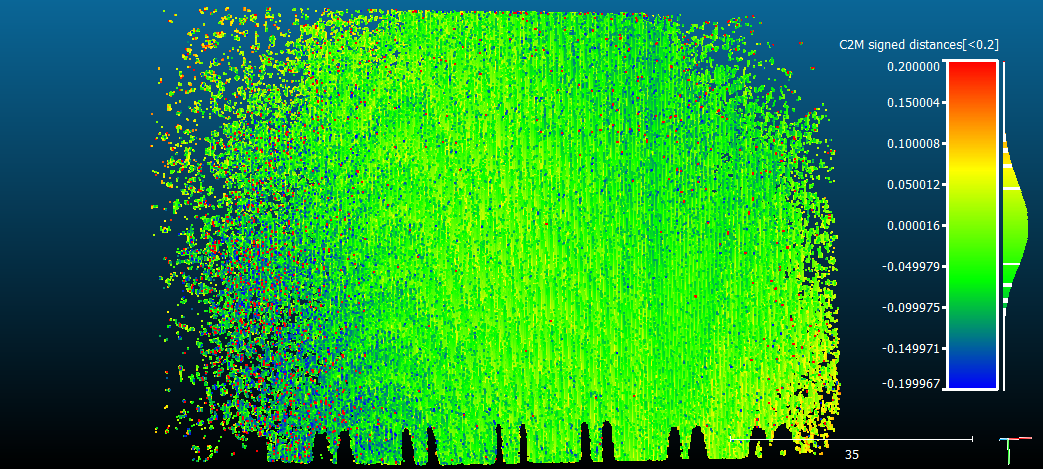
\includegraphics[width=1.0\linewidth]{scans/patronPlanicidad/2014.11.10_16.01.38/planeError_max200um}
        }
        \caption{Diversas vistas de las mediciones del objeto plano}
        \label{fig:planeScanViews1}
\end{figure}

\begin{figure}[!bth]
    \myfloatalign
        \subfloat[Medicion del patrón de planicidad a $\approx$24cm]{
            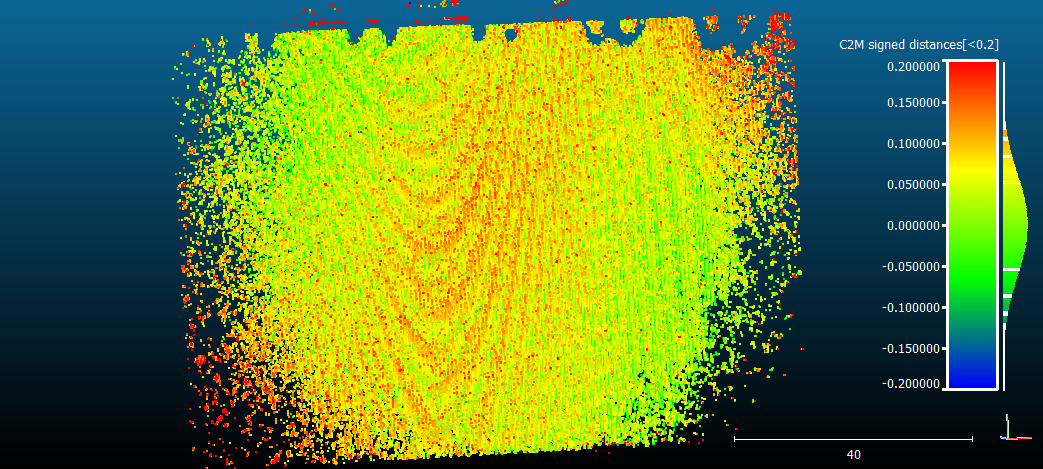
\includegraphics[width=1.0\linewidth]{scans/patronPlanicidad/2014.11.10_15.02.37/planeError_max200um}
        }
        \\
        \subfloat[Medicion del patrón de planicidad a $\approx$26cm]{
            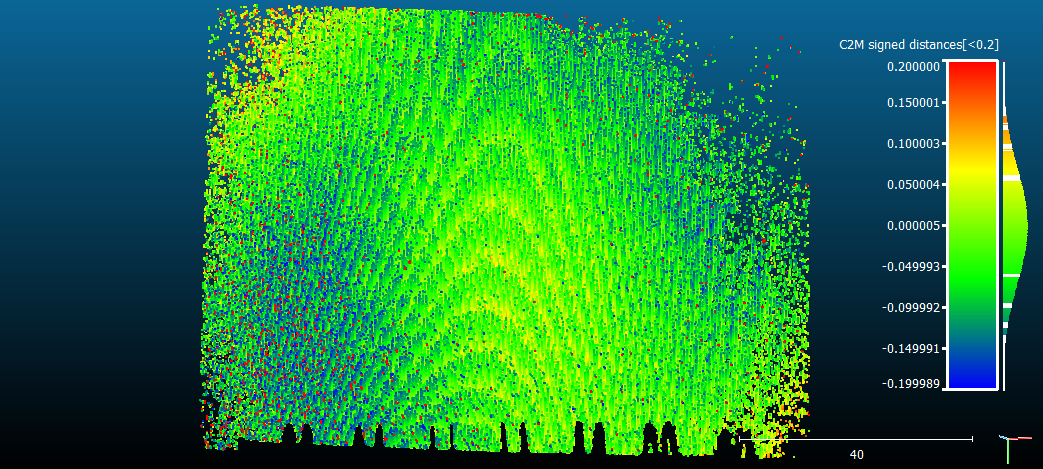
\includegraphics[width=1.0\linewidth]{scans/patronPlanicidad/2014.11.10_16.47.22/planeError_max200um}
        }
        \\
        \subfloat[Medicion del patrón de planicidad a $\approx$29cm]{
            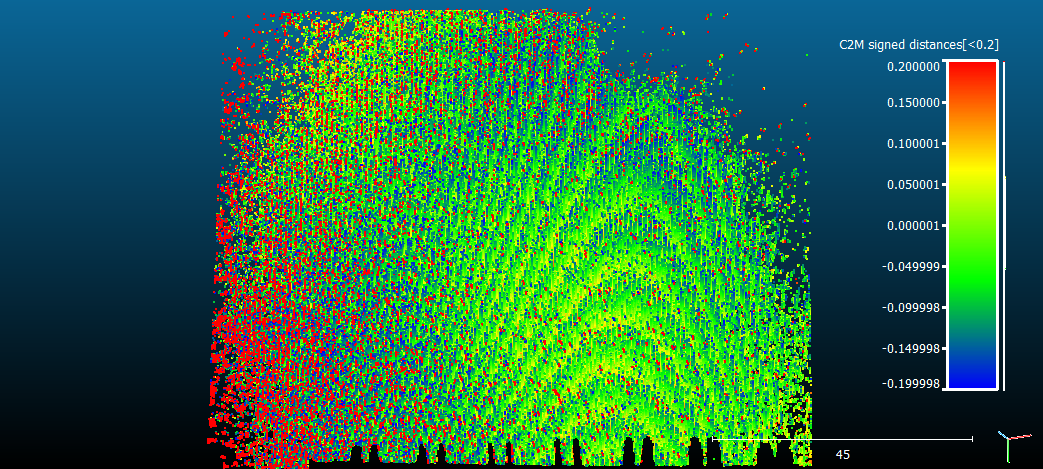
\includegraphics[width=1.0\linewidth]{scans/patronPlanicidad/2014.11.10_17.40.33/planeError_max200um}
        }
        \\
        \subfloat[Todas las mediciones del patrón de planicidad]{
            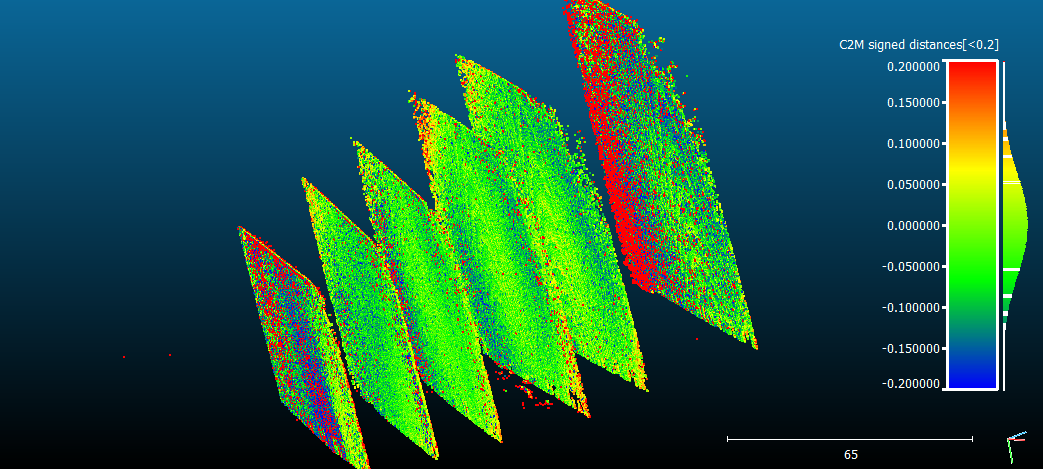
\includegraphics[width=1.0\linewidth]{scans/patronPlanicidad/all_planeError_max200um}
        }
        \caption{Diversas vistas de las mediciones del objeto plano (continuación)}
        \label{fig:planeScanViews2}
\end{figure}

\FloatBarrier % evita que los floats (figuras, tablas, etc) definidos arriba aparezcan despues de este lugar
\subsection{Objeto cilíndrico}
La cupla fue medida en seis distintas posiciones, y el desplazamiento fue realizado sobre una plataforma de desplazamiento lineal motorizada, abarcando un rango de $100$mm (una medición cada $20$mm). El desplazamiento se realiza sobre el eje $z$, en dirección alejándose del dispositivo de medición. En la \autoref{fig:setupCuplaRoja} se puede observar la cupla al momento de la medición.

\begin{figure}[!bth]
    \myfloatalign
        {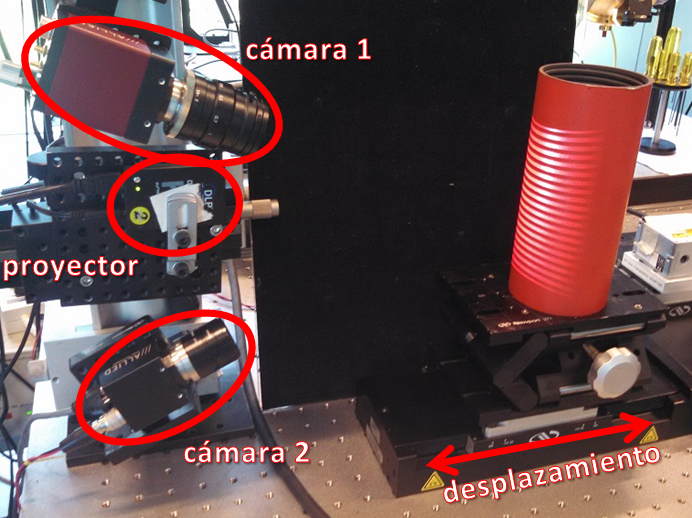
\includegraphics[width=1.0\linewidth]{images/setup/setup_cupla_explicado}}
        \caption{Medición de una cupla}
        \label{fig:setupCuplaRoja}
\end{figure}

Para cada medición se realiza una aproximación del cilindro que minimiza el error, y en este caso no sólo observaremos la variación de los puntos respecto al cilindro ajustado sino también el radio, la ubicación y la orientación de éste.

En la \autoref{tab:cylinderResults} se muestra el radio estimado y su error respecto al real. El desvío estándar corresponde a la diferencia entre la nube de puntos y la superficie del cilindro aproximado. El diametro del cilindro real es aproximadamente $82.5$mm, con lo cual su radio es aproximadamente $41.25$mm. 
Se puede ver que el cilindro estimado representa un error relativamente bajo (alrededor de los $0.5$mm) pese a que solamente estamos observando una sección de la curvatura del objeto. En la \autoref{fig:cylinderRadiusErrorVsDistance} se muestra un gráfico donde se puede observar la variación del error respecto a la distancia entre el dispositivo de medición y el objeto.
% La sobreestimación del radio de un círculo/cilindro es un hecho comunmente observado cuando solamente se utiliza información de una sección de éste.
Por otro lado el desvío estándar observado es menor a $0.1$mm, lo cual representa menos del $0.1$\% del rango de medición (el cual es mayor a los más de $100$mm que abarcamos con el desplazamiento del objeto). En la \autoref{fig:cylinderFitErrorDistribution} se puede observar la distribución del error y en la \autoref{fig:cylinderFitErrorVsDistance} se puede observar la variación del desvío estándar respecto a la distancia a la que se realiza la medición.

\begin{table}[!bth] 
    \myfloatalign
    \begin{tabularx}{\textwidth}{ X | c | c | c | c | c | c }
    & \multicolumn{6}{c}{Distancia de medición [mm]} \\
    & \rotatebox{0}{\shortstack[l]{210}} 
     & \rotatebox{0}{\shortstack[l]{230}} 
     & \rotatebox{0}{\shortstack[l]{250}} 
     & \rotatebox{0}{\shortstack[l]{270}} 
     & \rotatebox{0}{\shortstack[l]{290}} 
     & \rotatebox{0}{\shortstack[l]{310}} \\ 
    \hline
    Radio [mm] & $41.82$ & $41.82$ & $41.81$ & $41.79$ & $41.77$ & $41.74$ \\ 
    \hline
    Error en radio [mm] & $0.57$ & $0.56$ & $0.55$ & $0.54$ & $0.51$ & $0.49$ \\
%    \hline
%    Error medio superficie [um] & $0.2$ & $0.1$ & $-0.1$ & $-0.1$ & $-0.2$ & $4.2$ \\ 
    \hline
    Desvío estandar [um] & $46.4$ & $49.6$ & $55.7$ & $65.7$ & $80$ & $92.2$ \\ 
    \hline
    \end{tabularx}
    \caption{Resultados de la medición del objeto cilíndrico}
    \label{tab:cylinderResults}
\end{table}

\begin{figure}[!bth]
    \myfloatalign
        {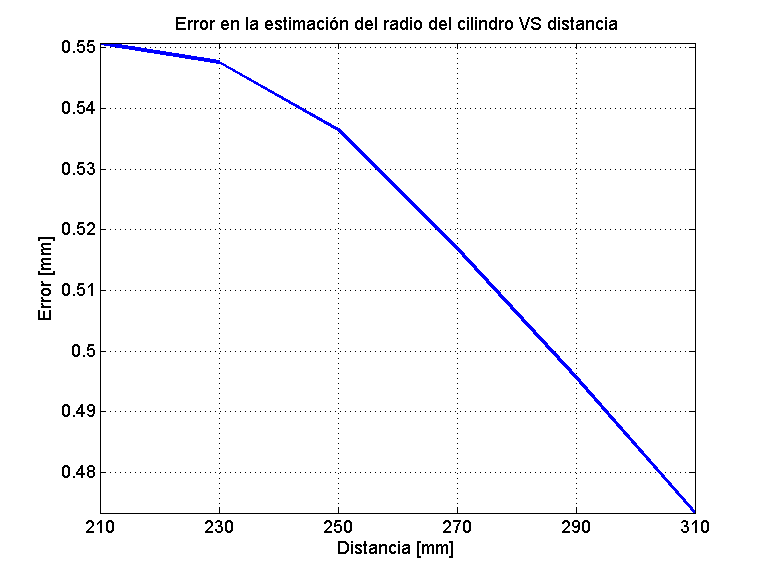
\includegraphics[width=1.0\linewidth]{scans/plotCylinderRadiusError}}
        \caption{Objeto cilíndrico: error en la estimación del radio en función de la distancia}
        \label{fig:cylinderRadiusErrorVsDistance}
\end{figure}

\begin{figure}[!bth]
    \myfloatalign
        {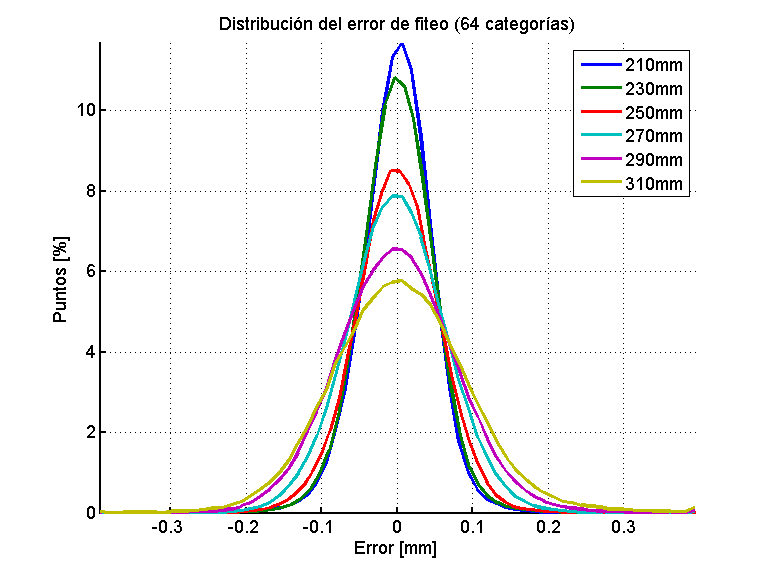
\includegraphics[width=1.0\linewidth]{scans/plotCylinder}}
        \caption{Objeto cilíndrico: distribución del error}
        \label{fig:cylinderFitErrorDistribution}
\end{figure}

\begin{figure}[!bth]
    \myfloatalign
        {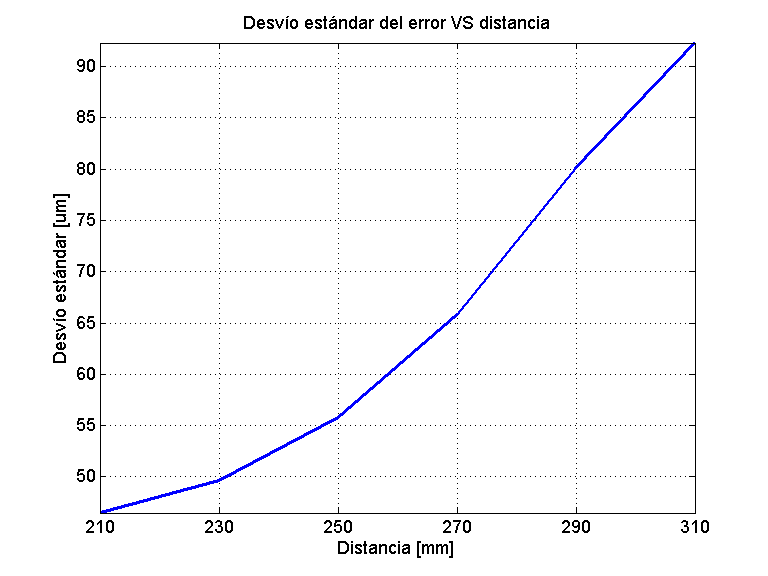
\includegraphics[width=1.0\linewidth]{scans/plotCylinderSD}}
        \caption{Objeto cilíndrico: desvío estándar del error en función de la distancia}
        \label{fig:cylinderFitErrorVsDistance}
\end{figure}


Otro resultado interesante de observar es la ubicación espacial del objeto, tanto la distancia observada entre el objeto y el dispositivo de medición como su orientación. Como el movimiento del objeto fue realizado sobre una plataforma de desplazamiento lineal motorizada de buena precisión, podemos asumir que todo el error observado corresponde a errores del dispositivo de medición. Para analizar este caso utilizaremos la aproximación del cilindro obtenido a partir de la nube de puntos. En la \autoref{tab:cylinderDirectionAndLocationResults} se pueden observar los resultados obtenidos.  

La orientación puede ser analizada a partir de la dirección del eje del cilindro ajustado. En la \autoref{fig:cylinderDirectionErrorVsDistance} se puede observar la diferencia entre los ejes de los cilindros detectados en cada medición. La diferencia corresponde al ángulo entre los ejes. Se considera que el cilindro correspondiente a la menor distancia de medición es el que presenta el menor error, por lo cual es usado como referencia. Se puede observar que la diferencia de cada eje respecto al primero es despreciable, siendo la máxima alrededor de $0.06$°.

La distancia entre los cilindros detectados en cada medición se debe calcular en la misma dirección en que se realizó el desplazamiento, para ello utilizaremos una dirección perpendicular a la dirección media entre todos los ejes, debido a que el objeto se desplazó de esta manera. Los puntos entre los cuales se calcula la distancia corresponden a la intersección del eje de cada cilindro contra un plano centrado en las mediciones observadas y cuya normal corresponde a la media entre los ejes. En la \autoref{fig:cylinderLocationErrorVsDistance} se puede observar la distancia entre los ejes de cada cilindro, nuevamente tomando como referencia el cilindro correspondiente a la menor distancia de medición. Se puede notar que el error se va acumulando y el error máximo es el observado entre los extremos, es decir entre la medición a $\approx210$mm y la medición a $\approx310$mm, el cual es menor a los 0.2mm.

\begin{table}[!bth] 
    \myfloatalign
    \begin{tabularx}{\textwidth}{ l X | c | c | c | c | c | c }
    & & \multicolumn{6}{c}{Distancia de medición [mm]} \\
    & & \rotatebox{0}{\shortstack[l]{210}} 
       & \rotatebox{0}{\shortstack[l]{230}} 
       & \rotatebox{0}{\shortstack[l]{250}} 
       & \rotatebox{0}{\shortstack[l]{270}} 
       & \rotatebox{0}{\shortstack[l]{290}} 
       & \rotatebox{0}{\shortstack[l]{310}} \\ 
    \hline 
    & x
	& $0.9232$
	& $-0.9233$
	& $-0.9234$
	& $0.9235$
	& $0.9235$
	& $-0.9236$ \\[1ex]
%    \hline
    & y
	& $0.0362$
	& $-0.0362$
	& $-0.0361$
	& $0.0362$
	& $0.0361$
	& $-0.0364$ \\[1ex]
%    \hline
    \rotatebox{90}{\rlap{Orientación}} 
    & z
	& $-0.3825$
	& $0.3823$
	& $0.3821$
	& $-0.3818$
	& $-0.3816$
	& $0.3815$ \\[1ex]
    \hline
    & x 
	& $13.449$
	& $88.428$
	& $78.929$
	& $13.324$
	& $-5.107$
	& $47.075$ \\[1ex]
%    \hline
    & y
	& $-10.954$
	& $-9.924$
	& $-12.211$
	& $-16.699$
	& $-19.335$
	& $-19.213$ \\[1ex]
%    \hline
    \rotatebox{90}{\rlap{Ubicación}} 
    & z
	& $272.831$
	& $263.345$
	& $288.836$
	& $337.504$
	& $366.628$
	& $366.578$ \\[1ex]
    \hline
    \end{tabularx}
    \caption{Orientación y ubicación espacial (punto sobre el eje) del cilindro}
    \label{tab:cylinderDirectionAndLocationResults}
\end{table}


\begin{figure}[!bth]
    \myfloatalign
        {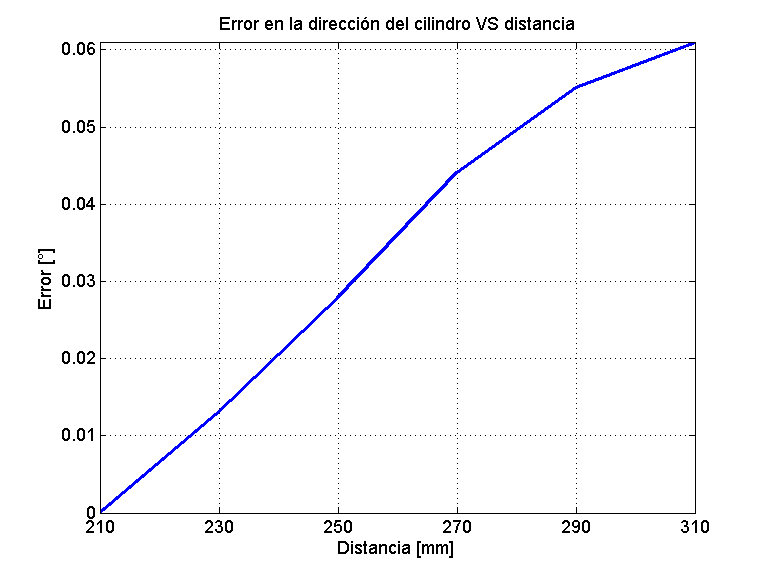
\includegraphics[width=1.0\linewidth]{scans/plotCylinderDirectionError}}
        \caption{Objeto cilíndrico: error en la orientación del cilindro en función de la distancia}
        \label{fig:cylinderDirectionErrorVsDistance}
\end{figure}

\begin{figure}[!bth]
    \myfloatalign
        {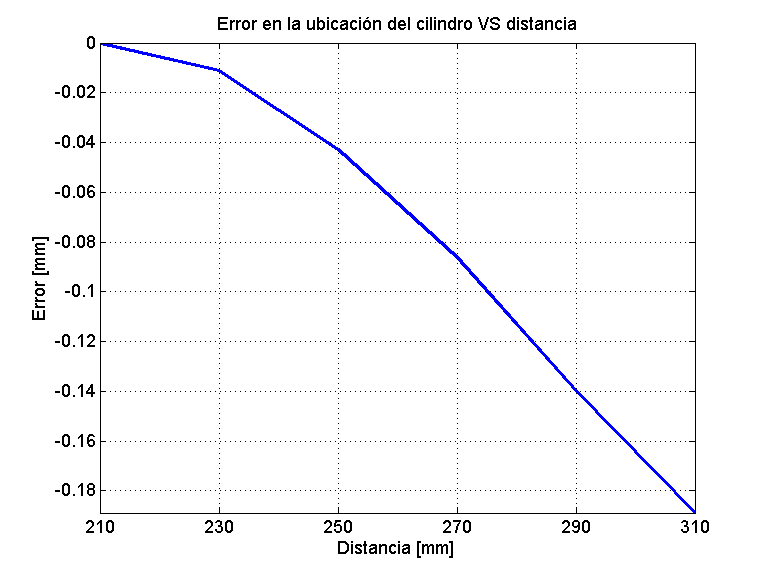
\includegraphics[width=1.0\linewidth]{scans/plotCylinderLocationError}}
        \caption{Objeto cilíndrico: error en la ubicación espacial del cilindro en función de la distancia}
        \label{fig:cylinderLocationErrorVsDistance}
\end{figure}

En la \autoref{fig:cylinderScanViews} se pueden observar distintas vistas de las nubes de puntos obtenidas para cada ubicación junto con la aproximación del cilindro completo. 
Nuevamente el color de cada punto corresponde al error respecto al cilindro fiteado, y en la parte inferior de cada imágen se puede observar la escala de colores. Estas imágenes fueron obtenidas con el software desarrollado en este trabajo.

Se puede notar que en cada medición se obtiene información sobre aproximadamente una cuarta parte de la circunferencia del objeto cilíndrico. Esta es toda la información que utilizamos para realizar una aproximación del cilindro completo, lo que nos permite obtener una estimación de su radio y su ubicación en el espacio.

\begin{figure}[!bth]
    \myfloatalign
        \subfloat{
            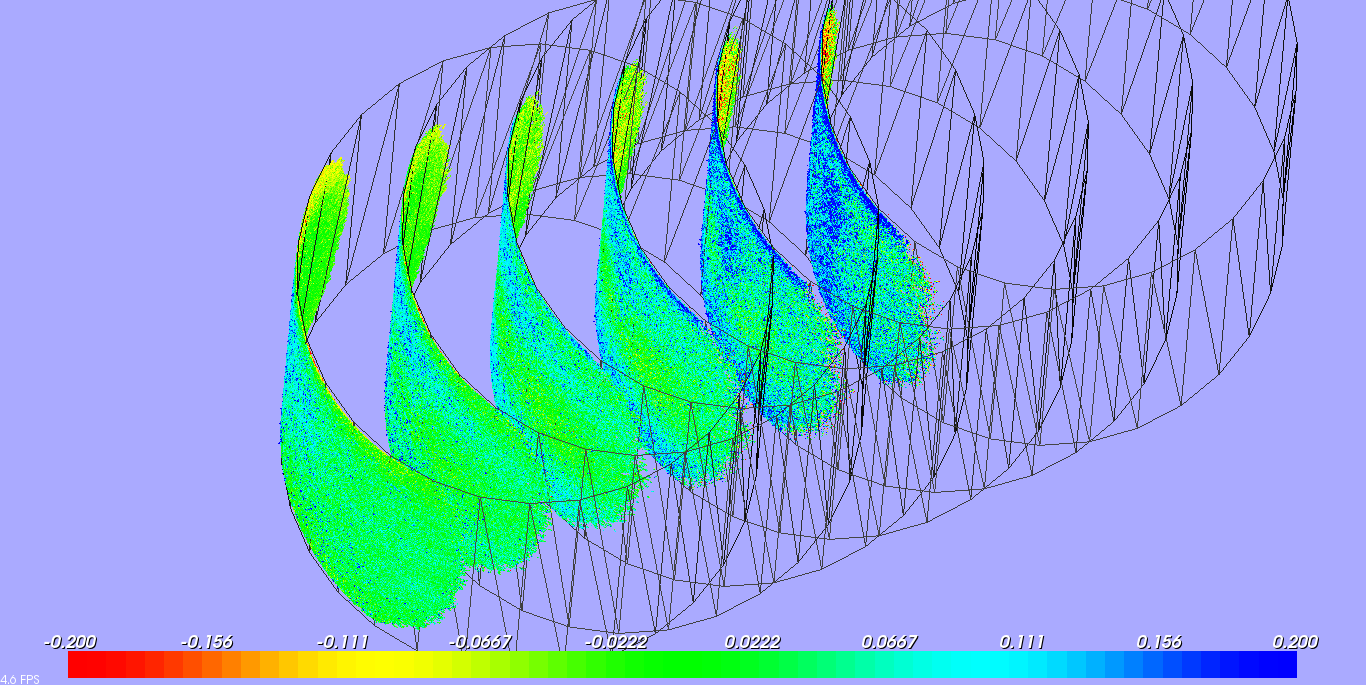
\includegraphics[width=0.9\linewidth]{scans/cupla_desplazamiento/woPostProc_3}
        }
        \\
        \subfloat{
            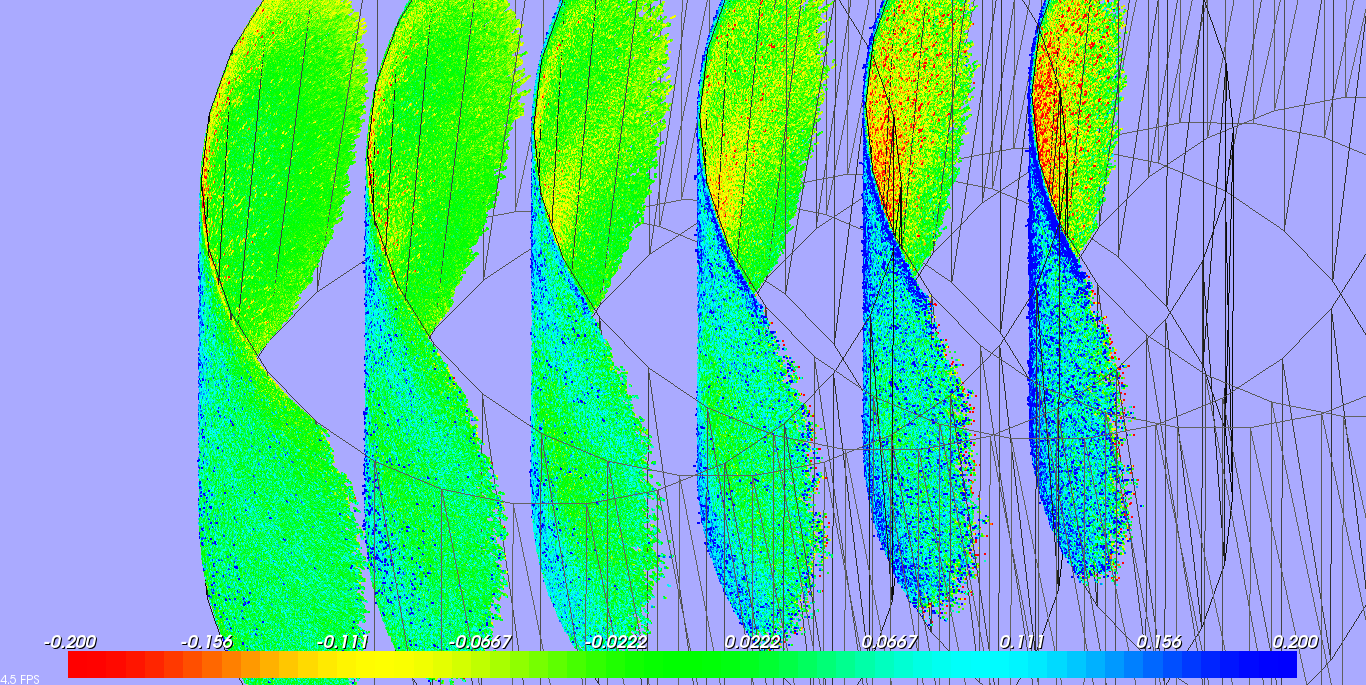
\includegraphics[width=0.9\linewidth]{scans/cupla_desplazamiento/woPostProc_5}
        }
        \\
        \subfloat{
            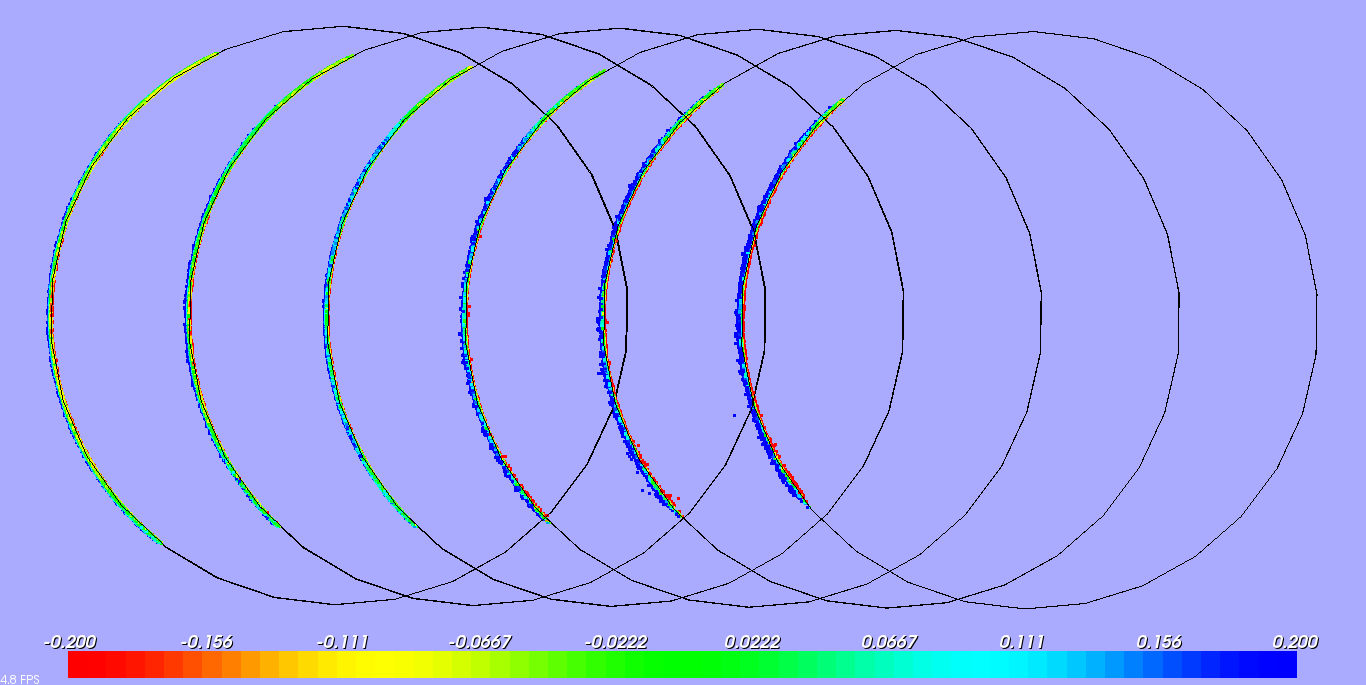
\includegraphics[width=0.9\linewidth]{scans/cupla_desplazamiento/woPostProc_2}
        }
        \\
        \subfloat{
            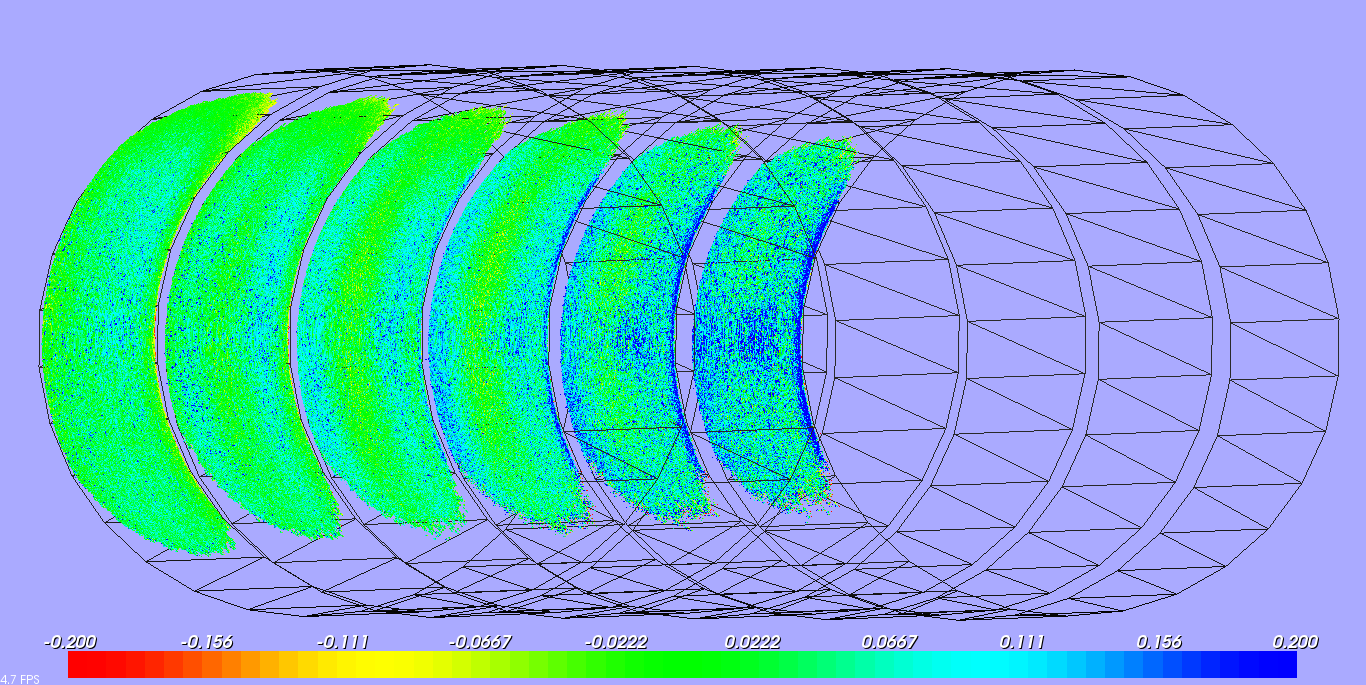
\includegraphics[width=0.9\linewidth]{scans/cupla_desplazamiento/woPostProc_1}
        }
        \caption{Diversas vistas de las mediciones del objeto cilíndrico}
        \label{fig:cylinderScanViews}
\end{figure}



%\section{Estimación del error}


%*****************************************
%*****************************************
%*****************************************
%*****************************************
%*****************************************




